% Generic System and Software Architecture Design Template
% Developed by Darian Muresan, Ph.D.
% In conjunction with the AI agents OpenAI Codex and Anthropic Claude Code.
% dmuresan@stevens.edu
% darian@dmmd.net
% darian@pictomic.com
% AI agents: read s8sAIAgentGuide.tex before editing this template.
\documentclass[12pt]{cornell}

\usepackage[T1]{fontenc}
\usepackage{lmodern}
\usepackage{xspace}
\usepackage{xcolor}
\usepackage{graphicx}
\usepackage{tikz}
\usetikzlibrary{arrows.meta,calc,fit,positioning,shapes.geometric}
\usepackage{fancyhdr}
\usepackage{amsmath,amssymb}
\usepackage{array}
\usepackage{booktabs}
\usepackage{longtable}
\usepackage{tabularx}
\usepackage{ltablex}
\keepXColumns
\usepackage{enumitem}
\usepackage{needspace}
\usepackage{listings}
\usepackage{pdflscape}
\usepackage{tcolorbox}
\usepackage{makeidx}
\usepackage[colorlinks=true,citecolor=blue,linkcolor=blue,urlcolor=blue]{hyperref}
\usepackage[acronym,toc]{glossaries}

\makeatletter
\renewcommand*{\l@subsection}{\@dottedtocline{2}{3.8em}{4.0em}}
\makeatother

\makeindex
\makeglossaries
\newacronym{ai}{AI}{artificial intelligence}
\newacronym{ui}{UI}{user interface}
\newacronym{uml}{UML}{Unified Modeling Language}
\newacronym{vnv}{V\&V}{verification and validation}

\newglossaryentry{acceptancecriterion}{
  name={acceptance criterion},
  description={An observable condition used to decide whether a need, story, or requirement has been satisfied}
}
\newglossaryentry{must}{
  name={Must},
  description={A capability required in the current release; the release is unacceptable without it}
}
\newglossaryentry{should}{
  name={Should},
  description={An important capability expected in the current release unless a documented constraint prevents it}
}
\newglossaryentry{could}{
  name={Could},
  description={A desirable capability included only when time and resources permit}
}
\newglossaryentry{would}{
  name={Would},
  description={A capability assigned to a later implementation version after higher-priority work}
}
\newglossaryentry{requirement}{
  name={requirement},
  description={A necessary, singular, unambiguous, feasible, and verifiable statement of capability or constraint}
}
\newglossaryentry{stakeholder}{
  name={stakeholder},
  description={A person, group, or organization that affects the system or is affected by it}
}
\newglossaryentry{traceability}{
  name={traceability},
  description={The ability to follow an artifact backward to its source and forward to its implementation and evidence}
}
\newglossaryentry{usecase}{
  name={use case},
  description={A goal-oriented interaction between an actor and the system, including normal and alternate flows}
}
\newglossaryentry{validation}{
  name={validation},
  description={Confirmation that the completed system satisfies stakeholder needs in its intended context; building the right system}
}
\newglossaryentry{verification}{
  name={verification},
  description={Confirmation that specified requirements have been fulfilled; building the system right}
}
\newglossaryentry{vmodel}{
  name={V-model},
  description={A lifecycle model that pairs each decomposition and specification activity with a corresponding integration and evidence activity}
}

\newglossaryentry{embeddedapplication}{name={embedded software application},description={The earlier scoped C++ acquisition software; execution target and allocation relative to interface logic remain open}}
\newglossaryentry{controlapp}{name={control app},description={The C++ macOS host application that receives associated conversion and counter data, qualifies measurements, and publishes results}}
\newglossaryentry{sample}{name={sensor sample},description={The measured data acquired through the ADC0804 path; physical units, timing, and qualification remain to be defined}}
\newglossaryentry{platformmatrix}{name={host platform matrix},description={The approved combinations of OS family, version, CPU architecture, and toolchain; coverage is not yet selected}}

\newglossaryentry{conversioncode}{name={conversion code},description={The 8-bit digital conversion output of the sensor-coupled ADC0804; analog scaling remains open}}
\newglossaryentry{countervalue}{name={counter value},description={The value supplied by the clock/counter alongside the conversion code; width, event association, rollover, and time meaning remain open}}
\newglossaryentry{interfacelogic}{name={interface logic},description={The responsibility for capture, association, and transfer of conversion/counter inputs into the FT245R data path; physical/software realization is unselected}}
\newglossaryentry{qualification}{name={measurement qualification},description={The host evaluation of whether a measurement can be used under rules that remain to be defined}}
\newglossaryentry{publishedresult}{name={published result},description={Code, status, and timing data emitted to the downstream consumer; field semantics and encoding remain open}}
\newglossaryentry{sourcehealth}{name={source operating health},description={Evidence of whether the defined acquisition source is operating properly; distinct from connection state, with criteria still open}}

\newglossaryentry{diagnosticrecording}{
  name={diagnostic recording},
  description={A persisted session of the samples, results, diagnostic events and capture context observed at an explicitly defined boundary for later investigation}
}
\newglossaryentry{playback}{
  name={playback},
  description={Delivery of recorded inputs through a defined processing boundary using explicit ordering, clock, state and output-routing rules; also called replay in user stories}
}


\definecolor{s8sBlue}{RGB}{31,78,121}
\definecolor{s8sGreen}{RGB}{46,125,50}
\definecolor{s8sRed}{RGB}{183,28,28}
\definecolor{s8sGray}{RGB}{90,90,90}
\definecolor{s8sLightBlue}{RGB}{232,240,247}

% Project metadata confirmed November 9, 2026.
% DocumentVersion retains template lineage; this is not a software release version.
\newcommand{\FileNamespace}{s8s}
\newcommand{\ProjectName}{SPE-800-Sensor}
\newcommand{\DocumentVersion}{2.33}
\newcommand{\DocumentStatus}{Draft}
\newcommand{\DocumentOwner}{Michael Stoddard}
\newcommand{\Organization}{Stevens Institute}
\newcommand{\DocumentDate}{November 9, 2026}
\newcommand{\VERSION}{Version \DocumentVersion}

\hypersetup{
  pdftitle={SPE-800-Sensor - System and Software Architecture Design},
  pdfauthor={Michael Stoddard},
  pdfcreator={Darian Muresan, Ph.D., with OpenAI Codex and Anthropic Claude Code},
  pdfsubject={System and software architecture design for SPE-800-Sensor},
  pdfkeywords={software architecture, requirements, traceability, verification, validation}
}

\newcolumntype{Y}{>{\raggedright\arraybackslash}X}
\newcolumntype{L}[1]{>{\raggedright\arraybackslash}p{#1}}
\setlength{\tabcolsep}{4pt}
\renewcommand{\arraystretch}{1.12}
\setlength{\LTpre}{6pt}
\setlength{\LTpost}{6pt}

% Stable IDs are authored explicitly so references survive chapter reordering.
\newcommand{\ArtifactLabel}[2]{\phantomsection\label{#1:#2}}
\newcommand{\ArtifactID}[2]{\texttt{#2}\ArtifactLabel{#1}{#2}\index{#1!#2}}
\newcommand{\ArtifactRef}[2]{\hyperref[#1:#2]{\texttt{#2}}}

\newcommand{\UserStoryID}[1]{\ArtifactID{UserStory}{#1}}
\newcommand{\UserStoryRef}[1]{\ArtifactRef{UserStory}{#1}}
\newcommand{\RequirementID}[1]{\ArtifactID{Requirement}{#1}}
\newcommand{\RequirementRef}[1]{\ArtifactRef{Requirement}{#1}}
\newcommand{\UseCaseID}[1]{\ArtifactID{UseCase}{#1}}
\newcommand{\UseCaseRef}[1]{\ArtifactRef{UseCase}{#1}}
\newcommand{\ArchitectureID}[1]{\ArtifactID{Architecture}{#1}}
\newcommand{\ArchitectureRef}[1]{\ArtifactRef{Architecture}{#1}}
\newcommand{\TestCaseID}[1]{\ArtifactID{TestCase}{#1}}
\newcommand{\TestCaseRef}[1]{\ArtifactRef{TestCase}{#1}}
\newcommand{\VerificationID}[1]{\ArtifactID{Verification}{#1}}
\newcommand{\VerificationRef}[1]{\ArtifactRef{Verification}{#1}}
\newcommand{\ValidationID}[1]{\ArtifactID{Validation}{#1}}
\newcommand{\ValidationRef}[1]{\ArtifactRef{Validation}{#1}}

\newcommand{\ChapterLabel}[1]{\label{Chapter:#1}}
\newcommand{\ChapterRef}[1]{\hyperref[Chapter:#1]{Chapter~\ref*{Chapter:#1}}}
\newcommand{\StatusPass}{\textbf{\footnotesize\textcolor{s8sGreen}{PASS}}}
\newcommand{\StatusPending}{\textbf{\footnotesize\textcolor{s8sGray}{PENDING}}}
\newcommand{\StatusFail}{\textbf{\footnotesize\textcolor{s8sRed}{FAIL}}}
\newcommand{\ReqStatusOpen}{\textbf{\textcolor{s8sGray}{Open}}}
\newcommand{\ReqStatusInProgress}{\textbf{\textcolor{s8sBlue}{In Progress}}}
\newcommand{\ReqStatusDone}{\textbf{\textcolor{s8sGreen}{Done}}}
\newcommand{\ReqStatusRetired}{\textbf{\textcolor{s8sGray}{Retired}}}
\newcommand{\NoVersion}{\ensuremath{\varnothing}}

\newtcolorbox{s8sNote}[1][]{
  colback=s8sLightBlue,
  colframe=s8sBlue,
  boxrule=0.6pt,
  arc=1mm,
  title=#1
}

\lstset{
  backgroundcolor=\color{white},
  basicstyle=\ttfamily\footnotesize,
  breaklines=true,
  frame=single,
  keywordstyle=\color{blue},
  commentstyle=\color{s8sGreen},
  numbers=left,
  numbersep=6pt,
  numberstyle=\tiny\color{s8sGray},
  showstringspaces=false,
  stringstyle=\color{s8sRed},
  tabsize=2
}

\changenormalspacing{\singlespacing}

% Selective draft build: uncomment and list include names without .tex.
% Keep this block commented for complete verification and release builds.
% \includeonly{
%   s8sPrologue,
%   s8sAIAgentGuide,
%   s8sRequirements,
%   s8sArchitectureOverview,
%   s8sTests
% }

\begin{document}

\pagenumbering{roman}
\singlespacing
% Front matter included after \begin{document}.
\title{\ProjectName\\[0.5em]\large System Requirements and\\Architecture Specification\\[1.5em]\normalsize\VERSION\\\DocumentStatus}
\author{\DocumentAuthors\\\Organization}
\conferraldate{}{\DocumentDate}
\copyrightholder{\Organization}
\copyrightyear{2026}
\maketitle

\begin{copyrightpage}
\copyright\ \Organization\ 2026 \\
ALL RIGHTS RESERVED \\[0.2in]
\hyperref[Chapter:DocumentHistory]{Document History (Appendix~\ref*{Chapter:DocumentHistory})}

\vspace{0.4in}
\noindent\textbf{Template attribution.}
\ChapterLabel{TemplateAttribution}
Derived from ArchitectureDesignTemplate 2.33, developed by
Darian Muresan, Ph.D., in conjunction with OpenAI Codex and
Anthropic Claude Code. Project-specific ownership is recorded above.
\end{copyrightpage}

\begin{abstract}
  This architecture revision describes a system whose mission is to determine whether a measurement can be used. A sensor coupled to an ADC0804 produces an 8-bit conversion code; a clock/counter provides a counter value. Interface logic will define capture, association, and transfer of these two logical inputs through an FT245R USB-to-parallel data path. A C++ control app on macOS qualifies the measurement and publishes code, status, and timing to a downstream consumer. Operator, Integrator, and Maintainer needs guide the candidate requirements. Capture coherence, timing meaning, qualification rules, result format, source-health evidence, and embedded C++ allocation remain owned questions. This stage is documentation only; product tests and stakeholder validation are not executed.

\end{abstract}

\contentspage
\tablelistpage
\figurelistpage


\setcounter{page}{1}
\pagenumbering{arabic}
\pagestyle{fancy}
\fancyhf{}
\renewcommand{\chaptermark}[1]{\markboth{#1}{}}
\lhead{\small Chapter \thechapter}
\chead{\small\nouppercase{\leftmark}}
\rhead{\small\thepage}
\lfoot{\small\ProjectName}
\cfoot{\small\copyright\ \Organization}
\rfoot{\small\VERSION}
\renewcommand{\headrulewidth}{0.4pt}
\renewcommand{\footrulewidth}{0.4pt}

\chapter{Purpose and Scope}
\ChapterLabel{Introduction}
\label{Section:IntroductionResponsibility}
This chapter establishes the purpose, scope, audience, and status of this specification.
\glsadd{acceptancecriterion}\glsadd{requirement}\glsadd{stakeholder}\glsadd{traceability}\glsadd{usecase}\glsadd{validation}\glsadd{verification}%


\section{Purpose}
This System Requirements and Architecture Specification records the
stakeholder needs, candidate obligations, selected architecture, and planned
verification and validation for \ProjectName. Requirements and design views
share stable references with the detailed test and evidence registers.
The authored LaTeX and editable diagram sources are authoritative; this PDF
is the integrated review publication.

\section{Scope and Boundaries}
The mission is to determine whether a measurement can be used. The system
includes the sensor and ADC0804 conversion path, clock/counter, interface
logic, FT245R USB transfer, and host-side measurement processing. The
Mission application is an external consumer. The distinction between the
whole system and the sensor processing subsystem is defined in
\hyperref[Section:MeasurementMission]{the system context}.

The current host architecture addresses macOS. The four-platform field-use
need in \UserStoryRef{US-03} remains partially covered pending
\hyperref[Question:Q-121]{Q-121}. C++ constraints remain subject to the
embedded execution allocation in \hyperref[Question:Q-116]{Q-116}.
No hardware construction, application implementation, or executed product
evidence is included in this documentation stage.

\section{Audience and Authority}
The Operator, Acquisition-Developer, Field-Engineer, and Mission-Integrator
concerns are defined in \hyperref[Table:StakeholderNeeds]{the stakeholder
register}. Michael Stoddard coordinates technical decisions and evidence
planning. Dr. Darian Muresan retains acceptance authority under
\hyperref[Table:ProjectOwners]{the owner register}. Publication layout and a
successful document build do not approve requirements or establish product
conformance.

\section{Document Status and Conventions}
This is a Draft, revision \DocumentVersion, dated \DocumentDate.
The revision identifies this document presentation; an accepted engineering
baseline remains subject to \hyperref[Question:Q-110]{Q-110}.
Template lineage 2.33 is provenance, not the project revision or a software
release version.

A statement containing \textbf{shall} expresses a candidate binding
obligation subject to its recorded lifecycle and approval conditions.
Priority uses \gls{must}, \gls{should}, \gls{could}, and \gls{would}; it is
separate from lifecycle status. TBD identifies an unresolved value or
contract. Pending verification or validation identifies missing executed
evidence, rather than a passing result.

\section{Document Organization}
\ChapterRef{SystemContext}, \ChapterRef{UserStories},
\ChapterRef{UseCases}, and \ChapterRef{Requirements} define the context,
needs, scenarios, and complete candidate requirement register.
\ChapterRef{ArchitectureOverview} and the logical, interface, interaction,
runtime, deployment, development, and implementation chapters describe the
current design and its unresolved allocations.
\ChapterRef{VerificationApproach} defines the evaluation approach;
\ChapterRef{DevelopmentPlan} owns risks, decisions, and review authority.

The appendices retain the full \hyperref[Table:ProjectTests]{test definitions},
\hyperref[Table:VerificationRegister]{verification register},
\hyperref[Table:ValidationRegister]{validation register},
\hyperref[Table:TraceabilityMatrix]{traceability matrix}, and
\ChapterRef{TestEvidence}. Each controlled statement has one source; links
connect its need, obligation, design, and planned evidence.
Repository authoring and AI guidance are maintained separately and are
excluded from this reader publication.

\chapter{Governance, Risks, and Open Decisions}
\ChapterLabel{DevelopmentPlan}
\label{Section:DevelopmentPlanResponsibility}
This chapter defines project ownership, decision gates, tailoring, and change control.


\section{Project Authorship}
\label{Section:ProjectAuthorship}
Project documentation is co-authored by \DocumentAuthors.
The user confirmed Chadwick Adebiyi as co-author of all project documents
on November 23, 2026. The authorship metadata applies to this integrated
specification and to project-authored supporting documents. Ownership,
decision coordination, and acceptance authority are recorded separately in
\hyperref[Table:ProjectOwners]{the owner register}.

\section{Confirmed Governance}
The user reconfirmed these assignments for SPE-800-Sensor on November 9, 2026. These roles remain in effect until changed by the project owner. Recording these assignments does not claim that technical acceptance has occurred.
\small
\begin{tabularx}{\linewidth}{L{4.0cm}Y}
\caption{Project Owners\label{Table:ProjectOwners}}\\
\toprule
Role & Assigned owner\\\midrule
\endfirsthead
\toprule
Role & Assigned owner\\\midrule
\endhead
\bottomrule
\endlastfoot
Document owner & Michael Stoddard\\
Organization & Stevens Institute\\
Technical owner & Michael Stoddard\\
Verification/validation owner & Michael Stoddard\\
Acceptance authority & Dr. Darian Muresan\\
\end{tabularx}
\normalsize

\Needspace{12\baselineskip}
\section{Domain Profile Selection}
\label{Section:DevelopmentPlanProfiles}
\small
\begin{tabularx}{\linewidth}{L{3cm}L{2.4cm}Y}
\caption{Project Domain Profile Decisions\label{Table:ProjectDomainProfiles}}\\
\toprule
Profile & Status & Rationale and decision provenance\\\midrule
\endfirsthead
\toprule
Profile & Status & Rationale and decision provenance\\\midrule
\endhead
\bottomrule
\endlastfoot
Embedded Systems & Applicable & Confirmed by the user November 9, 2026: the system includes sensor hardware, conversion, timing, and a hardware/software interface. Technical tailoring owner: Michael Stoddard. This is the only supplied profile; additional profiles require a separate decision.\\
\end{tabularx}
\normalsize

\section{Stage and Change Control}
This stage covers documentation only. The user confirmed the namespace \texttt{s8s}. Authored sources and editable diagrams in \path|Architecture/| are authoritative for this project; the reusable template remains separate. Independent technical review and acceptance remain human work. Repository authoring and AI execution guidance are maintained outside this publication.

Maintain the architecture in \path|Architecture/| within the SPE-800 repository. Changes use a branch and pull request against \texttt{main}. This candidate is pending document review. Michael Stoddard coordinates the document review; Dr. Darian Muresan retains technical acceptance authority. No approval or publication is inferred from a successful build.

\section{Owned Questions and Decision Gates}
\label{Section:OwnedQuestions}
Question ownership follows the supplied roles; it assigns responsibility for obtaining an answer and does not claim the owner has answered it. Each question below remains Open for the residual decisions explicitly stated. Supplied facts are acknowledged in the question rather than silently treating the entire topic as unresolved. Dependent design and implementation wait for their disposition. Decisions belong here once, and other chapters link to them.
\small
\begin{tabularx}{\linewidth}{L{1.3cm}L{3.1cm}Y}
\caption{Owned Questions\label{Table:OwnedQuestions}}\\
\toprule
ID & Owner & Question and impact\\\midrule
\endfirsthead
\toprule
ID & Owner & Question and impact\\\midrule
\endhead
\bottomrule
\endlastfoot
\phantomsection\label{Question:Q-101}Q-101 & Michael Stoddard & Confirmed: mission is measurement usability; stakeholders are Operator, Acquisition-Developer, Field-Engineer, and Mission-Integrator. Define the intended operating context and measurable stakeholder success for SPE-800-Sensor. Blocks final validation criteria.\\
\phantomsection\label{Question:Q-102}Q-102 & Michael Stoddard & Confirmed: ADC0804 produces an 8-bit conversion code; FT245R supplies the USB-to-parallel path. Select sensor/physical quantity, signal range and units, ADC reference and conversion clock/handshake, calibration, exact device/board revisions, and electrical compatibility. Blocks the schematic and analog acceptance limits.\\
\phantomsection\label{Question:Q-103}Q-103 & Michael Stoddard & Confirmed: two logical parallel inputs feed the interface logic and FT245R USB data path. Define bus ownership, strobes/handshake, transfer order, framing, record boundaries, error detection, loss and backpressure behavior. Blocks a realizable transfer contract; see \hyperref[Question:Q-112]{Q-112}.\\
\phantomsection\label{Question:Q-104}Q-104 & Michael Stoddard & Set sampling rate, capture skew, end-to-end latency, jitter, queue/resource budgets, power limits, and operating conditions with units and tolerances. Hardware selection alone does not supply project performance limits.\\
\phantomsection\label{Question:Q-105}Q-105 & Michael Stoddard & Confirmed: the host qualifies measurements and publishes code, status, and timing. Define the human interaction form, Operator decision presentation, Field-Engineer access, and whether configuration, storage, or reverse commands are needed. No GUI or command channel is selected.\\
\phantomsection\label{Question:Q-106}Q-106 & Michael Stoddard & Confirmed: the current host is macOS; Windows/Linux are outside this revision. Select macOS versions, CPU architectures, C++ standard, compilers, libraries, FT245R driver/API, permissions, packaging, and build tools. Blocks reproducible host builds.\\
\phantomsection\label{Question:Q-107}Q-107 & Michael Stoddard & Define startup, shutdown, reset, disconnect, malformed/partial records, invalid data, overflow, stalled operation, degraded behavior, safe states, recovery, and security/privacy boundaries. Fault detection and handling are not implied by the named devices.\\
\phantomsection\label{Question:Q-108}Q-108 & Michael Stoddard & Select reference analog inputs and conversion/counter vectors, fault fixtures, expected qualification/publication results, evidence retention, and representatives of all four stakeholders. Define executable procedures after the interface and decision contracts are accepted.\\
\phantomsection\label{Question:Q-109}Q-109 & Michael Stoddard & Assess manufacturing/provisioning, field updates, maintenance, environment, standards, and component lifecycle for the selected devices; propose coverage or non-applicability dispositions for acceptance-authority approval.\\
\phantomsection\label{Question:Q-110}Q-110 & Michael Stoddard & Propose milestones, risk dispositions, requirement priorities, and the next document baseline version; route this documentation candidate for technical acceptance.\\
\phantomsection\label{Question:Q-111}Q-111 & Michael Stoddard & Define counter width, clock source/frequency/accuracy, capture event, reset and rollover rules, clock-domain crossing, and the relation of counter value to measurement time. Blocks timing interpretation; the counter is not assumed to be 8-bit or an absolute timestamp.\\
\phantomsection\label{Question:Q-112}Q-112 & Michael Stoddard & Define when code and counter are captured, how coherence is ensured, how one association is identified across transfer, and what happens on conversion/counter transitions, reset, partial transfer, or overflow. Compare capture/latch/serialization alternatives after constraints are known; none is selected.\\
\phantomsection\label{Question:Q-113}Q-113 & Michael Stoddard & Define the host qualification rules for measurement usability, all decision inputs, units, freshness/integrity limits, boundary conditions, and unknown/unusable outcomes. Blocks the decision oracle and any usable-measurement claim.\\
\phantomsection\label{Question:Q-114}Q-114 & Michael Stoddard & The Mission application interface uses Open Mission Systems (OMS). Define the sample and sensor-status interfaces for both use cases. The \hyperref[Table:OMSStatusDecisions]{OMS status decisions} govern \RequirementRef{REQ-OMS-01}. Define published code meaning (conversion code versus another code), status semantics, timing fields/origin/units/rollover, association, schema/version/encoding, delivery transport, cadence, and incomplete/error result policy with the downstream consumer. Blocks Mission-Integrator interpretation and publication tests.\\
\phantomsection\label{Question:Q-115}Q-115 & Michael Stoddard & Define what source means (USB device, interface logic, ADC/sensor, clock/counter, or the complete chain), connection evidence, operating-health evidence, diagnostic coverage, reporting mechanism, stale/unknown handling, and false-positive limits. Blocks Field-Engineer acceptance; enumeration and data arrival alone do not establish full source health.\\
\phantomsection\label{Question:Q-116}Q-116 & Michael Stoddard & Allocate interface logic and embedded C++ responsibilities to selected hardware, firmware, or programmable logic, or explicitly revise the earlier embedded-application obligation. Do not infer an MCU, FPGA, or firmware requirement from FT245R selection. Blocks implementation decomposition and embedded-toolchain verification.\\
\phantomsection\label{Question:Q-117}Q-117 & Michael Stoddard & Confirm whether the adjacent \path|mseManual-V1.40.pdf| supplies project evidence or course guidance and identify any relevant sections before incorporating it.\\
\end{tabularx}
\normalsize

\section{OMS Status Interface Decisions}
\RequirementRef{REQ-OMS-01} remains Proposed pending resolution of the
TBD values below. The dates are proposed decision targets. Michael Stoddard
owns coordination of the decisions and records the program-approved values
and their sources before routing the requirement for approval.

\small
\begin{tabularx}{\linewidth}{YL{1.2cm}L{3.5cm}L{3.45cm}}
\caption{OMS Status Interface Decisions\label{Table:OMSStatusDecisions}}\\
\toprule
Decision & Value & Owner & Target decision date\\\midrule
\endfirsthead
\toprule
Decision & Value & Owner & Target decision date\\\midrule
\endhead
\bottomrule
\endlastfoot
OMS standard version & TBD & Michael Stoddard & December 2, 2026\\
CAL profile & TBD & Michael Stoddard & December 2, 2026\\
UCI message & TBD & Michael Stoddard & December 2, 2026\\
Valid, stale, and faulted status mapping & TBD & Michael Stoddard & December 2, 2026\\
Responsible mission gateway & TBD & Michael Stoddard & December 2, 2026\\
Derived sensor-status data product & TBD & Michael Stoddard & December 2, 2026\\
CAL service contract & TBD & Michael Stoddard & December 2, 2026\\
\end{tabularx}
\normalsize

\section{Technical Review Decision Agenda}
\label{Section:ReviewDecisions}
The answers below are TBD. Michael Stoddard owns coordination and records
the agreed answers with the affected stakeholders and acceptance authority.
The OMS status decisions retain their target dates in
\hyperref[Table:OMSStatusDecisions]{the OMS decision register}.

\subsection{High-Priority Decisions}

\paragraph{Q-118. Local and mission sample boundaries.}\label{Question:Q-118}
Who produces and consumes the local record, and who owns mission sample
publication? Is the local consumer the mission gateway, another component,
or an external client? Does the Mission application consume qualified samples
over OMS, and if so, which approved sample contract and delivery endpoint
apply? Which boundary do \RequirementRef{REQ-F-107} and
\RequirementRef{REQ-I-101} govern? Which field meanings, clocks, encodings,
sequence rollover, and invalid or incomplete record dispositions apply at
each boundary? Record the agreed endpoints and contract identifiers.

\paragraph{Q-119. Operator presentation.}\label{Question:Q-119}
Where does the Operator see the reading information? What should appear for
valid, invalid, unavailable, and stale readings, including whether the last
value remains visible? Is age measured from conversion-ready time, sample
capture, or another event? Specify units, display precision, update cadence,
and how unknown age is shown. Which observations and use decisions should
the Operator make in the reference cases for \ValidationRef{VAL-120}?

\paragraph{Q-120. Continuous delivery.}\label{Question:Q-120}
What input rates, burst lengths, run duration, and concurrent processing
loads represent intended operation? What minimum delivery rate, maximum
inter-reading gap, and loss, duplication, or reordering limits apply at the
Mission application? How much buffering is required, and what should
happen at saturation? Name the load fixture, observation point, and
reference stream for \ValidationRef{VAL-117}. Keep the 10 ms local
publication allocation distinct from mission delivery limits.

\paragraph{Q-121. Field platform coverage.}\label{Question:Q-121}
Which part of the subsystem must execute on macOS, iOS, Windows, and Linux?
Which operating-system versions, processor architectures, connection
methods, permissions, and drivers qualify on each? Which platforms are
required in the next baseline and which will be delivered later? Identify
the representative field devices and the connection and reading-receipt
success criteria for each platform. Reconcile the result with
\hyperref[Question:Q-106]{Q-106} and the macOS-only
\RequirementRef{REQ-C-103}.

\paragraph{Q-122. Readiness, validity, and stale state.}\label{Question:Q-122}
What edge or level constitutes one ready event, and how are multiple or
partial events handled? Which inputs classify a sample as valid, invalid,
or unqualified? Does an invalid or unqualified sample reset the stale
timer? What is reported before the first valid reading and at the 100 ms
boundary, including simultaneous arrival of a valid sample? What event
restores valid output after staleness or a fault? Provide expected
observations for the readiness and stale-state tests.

\subsection{Additional Decisions}

\paragraph{Q-123. Timing and measurement uncertainty.}\label{Question:Q-123}
Where are conversion-ready, timestamp capture, local publication, and
stale-state transition observed? How are corresponding events and records
matched? What clock synchronization, resolution, calibration, and maximum
measurement uncertainty are required? How should a result whose uncertainty
straddles the 10 ms, 100 ms, or 1 ms limit be classified? Identify the
approved test loads, fixtures, and repeat conditions.

\paragraph{Q-124. Endpoint replacement.}\label{Question:Q-124}
Which alternate sensor and Mission application qualify as compatible
replacements? Which configurations, adapters, or setup changes are permitted,
and which would count as redesign? What sample and status workflows must
succeed before and after each independent swap, and what record of the
changes establishes that the connection was reused?

\paragraph{Q-125. OMS status meaning.}\label{Question:Q-125}
Which combinations of connection and operating-health evidence map to valid,
stale, and faulted status? How are contradictory, ambiguous, or missing
observations handled, and which state has precedence when several apply?
For each approved state or transition, what should the gateway emit and what
should the Mission application infer? Record the applicable program values
and approval source in \hyperref[Table:OMSStatusDecisions]{the OMS decision
register} before advancing \RequirementRef{REQ-OMS-01}.

\paragraph{Q-126. Mission delivery degradation and recovery.}\label{Question:Q-126}
What should the Mission application observe during loss of sample input,
loss of OMS delivery, and restoration? During an outage, should the gateway
discard, retain, or coalesce samples and status, and how are gaps signaled?
What sample or status may be published first after restoration? Specify
loss, recovery-time, and freshness limits, and identify the test fixtures
and the observation points for both mission outputs.

\section{Recording and Playback Decisions}
\label{Section:RecordingPlaybackDecisions}
Owner: Michael Stoddard for each question below. Status: Open. Decisions require stakeholder review and the applicable acceptance-authority disposition before dependent implementation or quantitative verdicts.

\paragraph{Q-127. Recording boundary and fault policy.}\label{Question:Q-127}
Select the recording input boundary and schema, including received bytes or decoded records, invalid/partial inputs, sample/result associations, event order, start/stop boundaries, stop-and-flush behavior, file identity, capture-start processing state and any prehistory or checkpoint needed to reproduce it, known-gap representation, interrupted-file recovery, and storage-failure indications. Define retention, storage permissions, sensitive-data handling, and resource budgets; replay cannot recover physical or transfer observations that were not captured.

\paragraph{Q-128. Recording context and compatibility.}\label{Question:Q-128}
Define format/version identification, required software/configuration/calibration metadata, available versus unknown fields, context presentation, accepted compatibility combinations, treatment of missing initial-state information, corrupt/truncated-file classification, rejection reasons, and revalidation when a selected file changes. Identify compatible and incompatible fixtures and the expected disposition of each.

\paragraph{Q-129. Playback time, state, and controls.}\label{Question:Q-129}
Define the playback processing boundary, event tie-break and rollover rules, supported speeds relative to real time, the recorded-interval/speed timing reference and its treatment of speed-change and pause boundaries, timing-error limits in milliseconds, observation clock and uncertainty, pause/resume boundaries, valid seek locations, restoration strategy, initialization on every start/restart independent of prior live or replay sessions, transient-output disposition, single-step event meaning, presentation, and completion/failure behavior. Choose replay-clock semantics for freshness and timeouts during pause, stepping, speed changes, and seeking. Decide concurrency with live input; it is not assumed. Set state/output reference oracles, including recordings begun during operation and the disposition when their initial state cannot be established. Reset, captured-state restoration and prehistory replay remain alternatives pending approval. Software replay reproduces captured inputs, not the physical sensor or USB hardware.

\paragraph{Q-130. Replay identification and routing.}\label{Question:Q-130}
Agree how playback is identified at presentation and sample/status output boundaries, the test-consumer contract, endpoint selection and changes, handling of absent selection or delivery failure, and conditions for any mission endpoint. Reconcile with the OMS decisions; no unapproved OMS field or live mission delivery is selected by this proposal.

\paragraph{Q-131. Recording and playback acceptance budgets.}\label{Question:Q-131}
Approve sustained recording rate in records/s, burst rate and duration, minimum run duration in seconds or hours, storage allocation, recorder loss count/fraction and observation interval, allowed added live latency in milliseconds, allowed delivery-rate/gap degradation, and per-control response limits in milliseconds or seconds. Identify fixture sizes, concurrent loads, storage conditions, repeat counts, calibrated clocks and uncertainty/verdict rules. Agree the representative fault, stakeholder tasks and success criteria for the four use-case validations. These TBDs block quantitative verdicts; no numerical value is inferred from existing live-path timing allocations.

\section{Risks and Lifecycle Gates}
Unresolved capture coherence may pair a conversion with the wrong counter value. Undefined qualification or publication semantics may produce an unusable decision or a misinterpreted result. Source connection may be confused with source health. ADC0804 and FT245R are selected, but remaining electrical, timing, allocation, and macOS-version decisions still block detailed design and conformance claims. Owners and affected decisions are identified in \hyperref[Table:OwnedQuestions]{the question register}. No probabilities, severity ratings, schedules, or mitigations have been approved.

The documentation gate requires supported metadata, explicit gaps, consistent traceability, a complete build, visual inspection, and human review. Later needs, requirements, architecture, implementation, verification, validation, and software-release gates require their own evidence and authorized dispositions. Milestones remain \hyperref[Question:Q-110]{Q-110}.

\chapter{System Context}
\ChapterLabel{SystemContext}
\label{Section:SystemContextResponsibility}
This chapter defines the mission, system boundary, stakeholders, and external result boundary.
\glsadd{embeddedapplication}\glsadd{controlapp}\glsadd{sample}\glsadd{platformmatrix}\glsadd{conversioncode}\glsadd{countervalue}\glsadd{interfacelogic}\glsadd{qualification}\glsadd{publishedresult}\glsadd{sourcehealth}%


\index{measurement usability}\index{ADC0804}\index{FT245R}\index{Operator}\index{Mission-Integrator}\index{Field-Engineer}
\section{Mission and Boundary}
\label{Section:MeasurementMission}
The mission is to determine whether a measurement can be used. In
Figure~\ref{Figure:SensorContext}, the system of interest includes the
acquisition hardware and the primarily C++ control app on macOS, Windows 11, and iOS. The sensor, ADC0804,
clock/counter, interface logic, and FT245R are external to the control app.
The physical quantity enters the system at the sensor. The Mission application is external to the system. It receives qualified
sensor samples and sensor status through the Open Mission Systems (OMS)
interface. The \ChapterRef{UseCases} boundary is the sensor processing
subsystem, which receives samples from the external Sensor/FTDI hardware.
The arrows show the direction and content of the measurement flow. See
\ArchitectureRef{ARC-103} and \ArchitectureRef{ARC-104} for the allocation
and its requirement links.
\begin{figure}[!htbp]
\centering
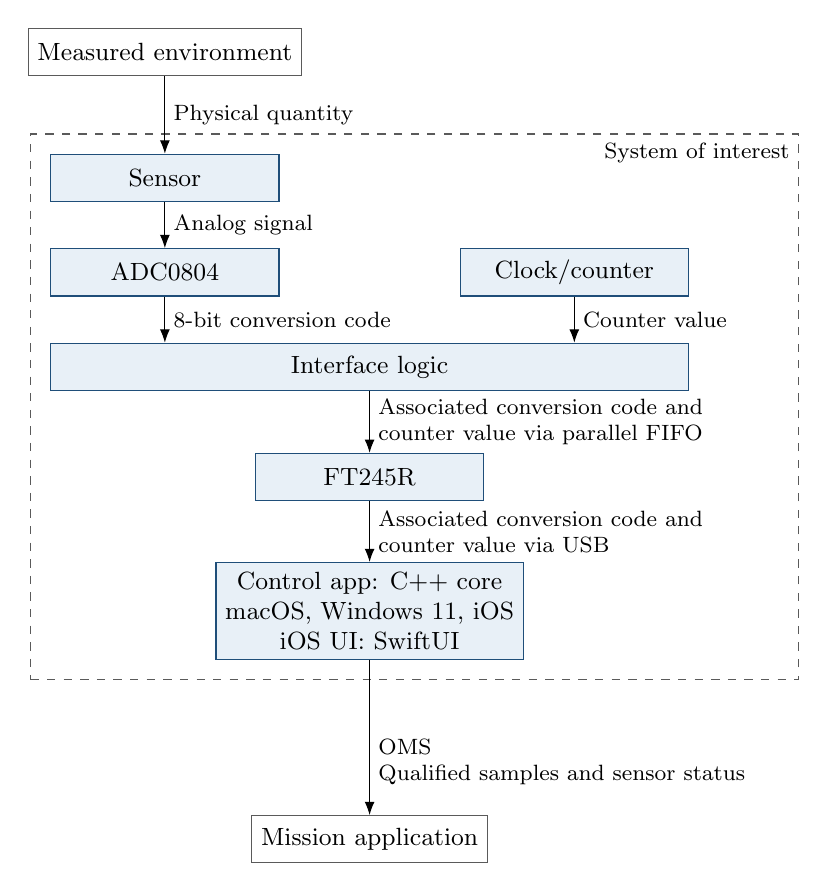
\begin{tikzpicture}[
  box/.style={draw=s8sBlue,fill=s8sLightBlue,align=center,
    minimum width=2.9cm,minimum height=0.6cm,font=\small},
  boundary/.style={draw=s8sGray,dashed,inner sep=0.25cm},
  flow/.style={->,>=Latex},
  data/.style={font=\footnotesize,align=left,inner sep=3pt}
]
\node[box,draw=s8sGray,fill=white] (environment) at (-2.6,0) {Measured environment};
\node[box] (sensor) at (-2.6,-1.6) {Sensor};
\node[box] (adc) at (-2.6,-2.8) {ADC0804};
\node[box] (counter) at (2.6,-2.8) {Clock/counter};
\node[box,minimum width=8.1cm] (logic) at (0,-4.0) {Interface logic};
\node[box] (ftdi) at (0,-5.4) {FT245R};
\node[box] (host) at (0,-7.1) {Control app: C++ core\\macOS, Windows 11, iOS\\iOS UI: SwiftUI};
\node[box,draw=s8sGray,fill=white] (consumer) at (0,-10.0) {Mission application};

\coordinate (right edge) at (5.2,-4);
\node[boundary,fit=(sensor)(adc)(counter)(logic)(ftdi)(host)(right edge)] (system) {};
\node[anchor=north east,font=\footnotesize,align=right] at (system.north east)
  {System of interest};

\draw[flow] (environment.south) -- node[data,right]{Physical quantity} (sensor.north);
\draw[flow] (sensor.south) -- node[data,right]{Analog signal} (adc.north);
\draw[flow] (adc.south) -- node[data,right]{8-bit conversion code}
  (adc.south |- logic.north);
\draw[flow] (counter.south) -- node[data,right]{Counter value}
  (counter.south |- logic.north);
\draw[flow] (logic.south) -- node[data,right]{Associated conversion code and\\counter value via parallel FIFO} (ftdi.north);
\draw[flow] (ftdi.south) -- node[data,right]{Associated conversion code and\\counter value via USB} (host.north);
\draw[flow] (host.south) -- node[data,right,pos=0.66]{OMS\\Qualified samples and sensor status} (consumer.north);
\end{tikzpicture}

\caption{Measurement flow across the acquisition hardware, control app, and Mission application boundaries.}
\label{Figure:SensorContext}
\end{figure}

\section{Boundary Information and Open Questions}
\label{Section:ContextBoundaryInformation}
\begin{description}[leftmargin=0pt,labelindent=0pt,labelsep=0pt,style=nextline]
\item[Physical quantity to sensor to ADC0804.]
The sensor responds to the physical quantity and supplies an analog signal
to the ADC0804. Identify the sensor and quantity, then establish the
operating conditions, signal units and range, conversion reference, and
calibration needed to interpret the conversion code
(\hyperref[Question:Q-101]{Q-101}, \hyperref[Question:Q-102]{Q-102}).

\item[ADC0804 and clock/counter to interface logic.]
The ADC0804 supplies an 8-bit conversion code \cite{ADC0804Datasheet}.
The clock/counter supplies a counter value through a separate logical input.
Define the counter width, clock, capture event, reset, rollover, and
relationship to measurement time. Establish how the interface logic associates
the code with the correct counter value and how much capture skew is allowed
(\hyperref[Question:Q-111]{Q-111}, \hyperref[Question:Q-112]{Q-112},
\hyperref[Question:Q-104]{Q-104}).

\item[Interface logic to FT245R.]
The interface logic sends the associated conversion code and counter value
through the FT245R parallel FIFO data path. The FT245R datasheet identifies
the D0--D7 data bus \cite{FT245RDatasheet}. Engineering must establish
electrical compatibility, bus ownership, handshake, transfer order,
record framing, and handling of incomplete transfers and backpressure
(\hyperref[Question:Q-102]{Q-102}, \hyperref[Question:Q-103]{Q-103},
\hyperref[Question:Q-112]{Q-112}).

\item[FT245R to control app.]
USB carries the associated conversion code and counter value to the control
app. Define platform-specific connection access, drivers and APIs for macOS, Windows 11, and iOS, reception and recovery behavior, and
the evidence and decision rules the control app uses to assess measurement
usability. Establish what observations support connection and operating-health
reporting and how the Field-Engineer receives that information
(\hyperref[Question:Q-106]{Q-106}, \hyperref[Question:Q-107]{Q-107},
\hyperref[Question:Q-113]{Q-113}, \hyperref[Question:Q-115]{Q-115}).

\item[Control app to Mission application.]
The control app qualifies measurement usability and supplies qualified samples
and sensor status to the Mission application over OMS. Define the applicable
OMS baseline, field semantics, timing origin and units, and delivery and
error handling with the Mission-Integrator
(\hyperref[Question:Q-114]{Q-114}).
\end{description}

The Operator's decision presentation and any configuration or reverse command
flow remain open in \hyperref[Question:Q-105]{Q-105}.

\section{Stakeholders}
\label{Section:MeasurementStakeholders}
The following roles define the sensor-system stakeholder set. The associated stories distinguish draft needs from the recording and playback needs accepted for inclusion in the story register. Stakeholder roles are distinct from engineering ownership in \hyperref[Table:ProjectOwners]{the owner register}.

\small
\begin{tabularx}{\linewidth}{L{3.6cm}Y}
\caption{Measurement Stakeholder Needs\label{Table:StakeholderNeeds}}\\
\toprule
Stakeholder & Need and story\\\midrule
\endfirsthead
\toprule
Stakeholder & Need and story\\\midrule
\endhead
\bottomrule
\endlastfoot
\phantomsection\label{Stakeholder:Operator}Operator & Needs to see sensor values and their validity, availability, and age so that they can decide whether to use each reading. \UserStoryRef{US-01}.\\
\phantomsection\label{Stakeholder:Acquisition-Developer}Acquisition-Developer & Needs sensor acquisition to continue while prior samples are processed so that mission software receives a continuous stream of readings. \UserStoryRef{US-02}. Accepted diagnostic needs: \UserStoryRef{US-06}, \UserStoryRef{US-08}.\\
\phantomsection\label{Stakeholder:Field-Engineer}Field-Engineer & Needs the sensor subsystem to run on macOS, Windows 11, iOS, and Linux so that they can use any available computer in the field. \UserStoryRef{US-03}. Accepted diagnostic needs: \UserStoryRef{US-05}, \UserStoryRef{US-07}.\\
\phantomsection\label{Stakeholder:Mission-Integrator}Mission-Integrator & Needs a documented interface for sensor data and status so that they can replace the sensor or the mission consumer without redesigning the connection. \UserStoryRef{US-04}. Accepted diagnostic need: \UserStoryRef{US-09}.\\
\end{tabularx}
\normalsize

\section{Stage and Allocation Boundaries}
This stage remains documentation only; no circuit, firmware, host implementation, or product evidence is produced. The control app targets macOS, Windows 11, and iOS under \RequirementRef{REQ-C-103}. \UserStoryRef{US-03} calls for field operation on macOS, Windows 11, iOS, and Linux. The selected platform matrix and connection feasibility remain open in \hyperref[Question:Q-106]{Q-106} and \hyperref[Question:Q-121]{Q-121}; Linux remains an additional stakeholder request. The control-app core remains primarily C++ under \RequirementRef{REQ-C-102}, with an iOS SwiftUI UI under \RequirementRef{REQ-C-104}. The earlier embedded C++ direction remains. The execution target and responsibility of embedded software relative to interface logic remain \hyperref[Question:Q-116]{Q-116}. Selecting ADC0804 and FT245R does not select a processor, FPGA, microcontroller, multiplexer, or host driver. The control app is the host application throughout this book; its name does not imply reverse commands. The iOS UI is selected as SwiftUI; desktop UI technologies and screen-level behavior remain open.

\chapter{Stakeholder and User Stories}
\ChapterLabel{UserStories}
\section{Chapter Responsibility}
\label{Section:UserStoriesResponsibility}
Capture sensor-system stakeholder stories and their acceptance intent, including recording and playback for debugging.

\noindent\textbf{Expected result:} Stakeholder needs linked to candidate obligations and validation scenarios.

\section{Stakeholder Story Register}
The mission and role definitions are authoritative in \hyperref[Section:MeasurementMission]{the mission} and \hyperref[Table:StakeholderNeeds]{the stakeholder register}. Each story states a role, capability, and outcome. The original stories retain their proposed acceptance intent and priorities. The user accepted \UserStoryRef{US-05}, \UserStoryRef{US-06}, \UserStoryRef{US-07}, \UserStoryRef{US-08}, and \UserStoryRef{US-09} on November 23, 2026 for inclusion in this chapter. Their acceptance intent is recorded below; priority and unresolved engineering details remain pending. Acceptance of a story does not establish implementation, passing evidence, or approval of derived requirements. At the user's request, the replay-output story originally proposed as US-11 is numbered \UserStoryRef{US-09}, giving the included stories consecutive IDs.

\small
\begin{tabularx}{\linewidth}{L{1.8cm}Y}
\caption{User Story Register\label{Table:UserStories}}\\
\toprule
ID & Need, acceptance intent, and mappings\\\midrule
\endfirsthead
\toprule
ID & Need, acceptance intent, and mappings\\\midrule
\endhead
\bottomrule
\endlastfoot
\UserStoryID{US-01} & As an \hyperref[Stakeholder:Operator]{Operator}, I need to see sensor values and their validity, availability, and age so that I can decide whether to use each reading. Acceptance intent. The Operator can distinguish valid, invalid, unavailable, and stale readings and determine the age of an available reading. Define how age is measured and displayed and how validity and availability are represented in \hyperref[Question:Q-105]{Q-105} and \hyperref[Question:Q-113]{Q-113}. Proposed priority is \gls{must}. Requirements and scenarios. \RequirementRef{REQ-F-101}, \RequirementRef{REQ-F-102}, \RequirementRef{REQ-F-103}, \RequirementRef{REQ-C-101}, \RequirementRef{REQ-C-102}, \RequirementRef{REQ-C-103}, \RequirementRef{REQ-F-104}, \RequirementRef{REQ-F-105}, \RequirementRef{REQ-F-106}, \RequirementRef{REQ-F-107}, \RequirementRef{REQ-F-108}, \RequirementRef{REQ-F-109}. Use cases: \UseCaseRef{UC-01}, \UseCaseRef{UC-02}. Added candidate mappings include \RequirementRef{REQ-SMP-01}, \RequirementRef{REQ-SMP-02}, \RequirementRef{REQ-TIM-02}, \RequirementRef{REQ-F-110}. See the \hyperref[Table:ValidationRegister]{requirement-level validation register}.\\
\UserStoryID{US-02} & As an \hyperref[Stakeholder:Acquisition-Developer]{Acquisition-Developer}, I need sensor acquisition to continue while prior samples are processed so that mission software receives a continuous stream of readings. Acceptance intent. With earlier samples still being processed, acquisition continues and mission software receives readings at the agreed cadence. Define the supported processing load and allowable gaps in \hyperref[Question:Q-104]{Q-104}. Existing acquisition and publication mappings cover parts of the data path. Proposed priority is \gls{must}. Requirements and scenarios. \RequirementRef{REQ-F-101}, \RequirementRef{REQ-F-102}, \RequirementRef{REQ-F-103}, \RequirementRef{REQ-F-104}, \RequirementRef{REQ-F-105}, \RequirementRef{REQ-F-107}. See \UseCaseRef{UC-01}. Added candidate mappings include \RequirementRef{REQ-SMP-01}, \RequirementRef{REQ-TIM-01}. See the \hyperref[Table:ValidationRegister]{requirement-level validation register}.\\
\UserStoryID{US-03} & As a \hyperref[Stakeholder:Field-Engineer]{Field-Engineer}, I need the sensor subsystem to run on macOS, iOS, Windows, and Linux so that I can use any available computer in the field. Acceptance intent. On each platform, a representative field computer can connect to the sensor subsystem and receive readings. Define supported versions, devices, and connection methods. The existing macOS-only candidate requirement \RequirementRef{REQ-C-103} is partial coverage. Cross-platform use case and validation mappings are pending the platform dispositions in \hyperref[Question:Q-121]{Q-121}. Proposed priority is \gls{must}.\\
\UserStoryID{US-04} & As a \hyperref[Stakeholder:Mission-Integrator]{Mission-Integrator}, I need a documented interface for sensor data and status so that I can replace the sensor or the mission consumer without redesigning the connection. Acceptance intent. Swap the sensor and the mission consumer independently for compatible replacements and confirm that the documented connection contract still applies. Define the sensor-side and mission-consumer-side compatibility criteria in \hyperref[Question:Q-102]{Q-102} and \hyperref[Question:Q-114]{Q-114}. The published result mappings cover the mission-consumer side. Proposed priority is \gls{must}. Requirements and scenarios. \RequirementRef{REQ-F-107}, \RequirementRef{REQ-I-101}. Use cases: \UseCaseRef{UC-01}. Added candidate mappings include \RequirementRef{REQ-IF-01}, \RequirementRef{REQ-OMS-01}, \UseCaseRef{UC-02}. See the \hyperref[Table:ValidationRegister]{requirement-level validation register}.\\
\UserStoryID{US-05} & \textbf{Record a session.} As a \hyperref[Stakeholder:Field-Engineer]{Field-Engineer}, I need to record sensor data and diagnostic events during operation so that I can investigate a fault after it occurs. Acceptance intent. Start and stop a recording; save received conversion codes, associated counter values, available timestamps and sequence numbers, qualification results, and connection/health events. Identify gaps and recording failures. Status: accepted for inclusion November 23, 2026. Priority: pending stakeholder prioritization. Open detail: recording boundary, supported recording rate and duration, storage limits, acceptable loss, and behavior when storage is unavailable or full. Requirements and scenarios: \RequirementRef{REQ-F-111}, \RequirementRef{REQ-F-112}, \RequirementRef{REQ-D-101}, \RequirementRef{REQ-F-113}, \RequirementRef{REQ-D-103}, \RequirementRef{REQ-Q-102}, \RequirementRef{REQ-Q-103}, \RequirementRef{REQ-Q-104}, \RequirementRef{REQ-Q-105}. Use cases: \UseCaseRef{UC-03}. Validation: \ValidationRef{VAL-121}. See \hyperref[Section:RecordingPlaybackTraceGaps]{coverage and remaining decisions}.\\
\UserStoryID{US-06} & \textbf{Replay a recorded session.} As an \hyperref[Stakeholder:Acquisition-Developer]{Acquisition-Developer}, I need to replay recorded inputs through the sensor processing software without connected sensor hardware so that I can reproduce and investigate observed software behavior. Acceptance intent. Load a supported recording and feed its inputs through the processing path in their recorded order. Preserve recorded timing relationships within agreed tolerances, including gaps and disconnect events. Status: accepted for inclusion November 23, 2026. Priority: pending stakeholder prioritization. Open detail: supported recording formats, replay input boundary, timing tolerances, clock behavior, and handling of incomplete or corrupt recordings. Requirements and scenarios: \RequirementRef{REQ-F-114}, \RequirementRef{REQ-F-115}, \RequirementRef{REQ-F-117}, \RequirementRef{REQ-F-127}, \RequirementRef{REQ-D-104}, \RequirementRef{REQ-Q-101}, \RequirementRef{REQ-F-126}. Use cases: \UseCaseRef{UC-04}, \UseCaseRef{UC-05}. Validation: \ValidationRef{VAL-122}, \ValidationRef{VAL-123}. See \hyperref[Section:RecordingPlaybackTraceGaps]{coverage and remaining decisions}.\\
\UserStoryID{US-07} & \textbf{Control playback.} As a \hyperref[Stakeholder:Field-Engineer]{Field-Engineer}, I need to pause, resume, change playback speed, and step through individual records so that I can examine the events surrounding a fault. Acceptance intent. Show playback position and the selected record's data and status. Define how seeking restores processing state and how playback speed affects freshness and timeout behavior. Status: accepted for inclusion November 23, 2026. Priority: pending stakeholder prioritization. Open detail: supported playback speeds, seek behavior, processing-state restoration, and the treatment of freshness and timeouts while paused or stepping. Requirements and scenarios: \RequirementRef{REQ-F-118}, \RequirementRef{REQ-F-119}, \RequirementRef{REQ-F-120}, \RequirementRef{REQ-F-121}, \RequirementRef{REQ-F-122}, \RequirementRef{REQ-F-123}, \RequirementRef{REQ-F-124}, \RequirementRef{REQ-F-125}, \RequirementRef{REQ-Q-106}. Use cases: \UseCaseRef{UC-06}. Validation: \ValidationRef{VAL-124}. See \hyperref[Section:RecordingPlaybackTraceGaps]{coverage and remaining decisions}.\\
\UserStoryID{US-08} & \textbf{Preserve diagnostic context.} As an \hyperref[Stakeholder:Acquisition-Developer]{Acquisition-Developer}, I need recordings to identify the software version, configuration, calibration, and data format used during capture so that I can interpret and reproduce the original processing conditions. Acceptance intent. Retain the agreed session metadata and identify missing or incompatible context before replay. Status: accepted for inclusion November 23, 2026. Priority: pending stakeholder prioritization. Open detail: required metadata, version identification, calibration/configuration representation, and compatibility rules. Requirements and scenarios: \RequirementRef{REQ-D-102}, \RequirementRef{REQ-F-114}, \RequirementRef{REQ-F-115}, \RequirementRef{REQ-F-116}. Use cases: \UseCaseRef{UC-03}, \UseCaseRef{UC-04}. Validation: \ValidationRef{VAL-121}, \ValidationRef{VAL-122}. See \hyperref[Section:RecordingPlaybackTraceGaps]{coverage and remaining decisions}.\\
\UserStoryID{US-09} & \textbf{Identify replay outputs.} As a \hyperref[Stakeholder:Mission-Integrator]{Mission-Integrator}, I need replayed samples and status to be distinguishable from live data so that I can test integration behavior without confusing recorded measurements with current measurements. Acceptance intent. Clearly indicate replay mode and define whether outputs go to a test consumer or an explicitly selected mission endpoint. Status: accepted for inclusion November 23, 2026. Priority: pending stakeholder prioritization. Open detail: replay identification at presentation and interface boundaries, endpoint selection, and applicable mission interface behavior. Requirements and scenarios: \RequirementRef{REQ-I-102}, \RequirementRef{REQ-I-103}. Use cases: \UseCaseRef{UC-05}. Validation: \ValidationRef{VAL-123}. See \hyperref[Section:RecordingPlaybackTraceGaps]{coverage and remaining decisions}.\\
\end{tabularx}
\normalsize

\chapter{System Requirements}
\ChapterLabel{Requirements}
\index{requirement}
\label{Section:RequirementsResponsibility}
This chapter specifies the candidate obligations for the measurement path and its users.


\section{Register Conventions}
Each row records its obligation, proposed priority, lifecycle status,
implementation version, originating need, use case, test, and open decisions.
Existing IDs are preserved, including the six user-assigned sensor-path IDs.
The normal identifier form is \path|REQ-[scope-]family-sequence|; the
user-assigned two-digit IDs remain explicit exceptions. No new family is
introduced by this publication change.

The register contains 18 Open requirements and two Proposed requirements.
Open records active scope for planning; it does not establish that referenced
contracts are resolved. Proposed records an obligation awaiting its approval
conditions. In Progress denotes implementation work; Done requires passing
tests, completed verification, current traceability, and a controlled
implementation version. Retired retains an obligation's history and ID.
All current implementation-version fields are empty because no product
implementation is recorded. Proposed Must priorities await review.

\section{Project Candidate Requirements}
The user-supplied measurement architecture refines the earlier candidate scope. Existing IDs are preserved. The acquisition path is no longer silently allocated entirely to embedded software; \RequirementRef{REQ-C-101} remains Open pending \hyperref[Question:Q-116]{Q-116}. The host scope in \RequirementRef{REQ-C-103} is revised from an unspecified macOS/Windows/Linux matrix to macOS. These changes are recorded in \ChapterRef{DocumentHistory}. All rows retain no implementation version and a proposed Must priority; the register records each row's Open or Proposed status. The named hardware does not complete detailed embedded tailoring or provide passing evidence.

Existing identifiers remain stable; new project IDs continue monotonically within each governed family.

\small
\begin{tabularx}{\linewidth}{L{2.5cm}Y}
\caption{Project Candidate Requirements\label{Table:ProjectRequirements}}\\
\toprule
ID & Obligation, lifecycle, trace links, and open detail\\\midrule
\endfirsthead
\toprule
ID & Obligation, lifecycle, trace links, and open detail\\\midrule
\endhead
\bottomrule
\endlastfoot
\RequirementID{REQ-F-101} & The acquisition path shall acquire the 8-bit conversion code produced by the sensor-coupled ADC0804. \textbf{Priority:} \gls{must} (proposed). \textbf{Status:} \ReqStatusOpen. \textbf{In Version:} \NoVersion. \textbf{Need:} \UserStoryRef{US-01}, \UserStoryRef{US-02}. \textbf{Use case:} \UseCaseRef{UC-01}. \textbf{Test:} \TestCaseRef{TC-101}. Open detail: \hyperref[Question:Q-102]{Q-102}, \hyperref[Question:Q-104]{Q-104}.\\
\RequirementID{REQ-F-102} & The acquisition path shall transfer acquired conversion data to the control app through the FT245R USB data path. \textbf{Priority:} \gls{must} (proposed). \textbf{Status:} \ReqStatusOpen. \textbf{In Version:} \NoVersion. \textbf{Need:} \UserStoryRef{US-01}, \UserStoryRef{US-02}. \textbf{Use case:} \UseCaseRef{UC-01}. \textbf{Test:} \TestCaseRef{TC-102}. Open detail: \hyperref[Question:Q-103]{Q-103}, \hyperref[Question:Q-112]{Q-112}.\\
\RequirementID{REQ-F-103} & The control app shall receive the conversion code and its associated counter value from the FT245R data path. \textbf{Priority:} \gls{must} (proposed). \textbf{Status:} \ReqStatusOpen. \textbf{In Version:} \NoVersion. \textbf{Need:} \UserStoryRef{US-01}, \UserStoryRef{US-02}. \textbf{Use case:} \UseCaseRef{UC-01}. \textbf{Test:} \TestCaseRef{TC-103}. Open detail: \hyperref[Question:Q-103]{Q-103}, \hyperref[Question:Q-111]{Q-111}, \hyperref[Question:Q-112]{Q-112}.\\
\RequirementID{REQ-C-101} & The embedded software application shall be developed in C++. \textbf{Priority:} \gls{must} (proposed). \textbf{Status:} \ReqStatusOpen. \textbf{In Version:} \NoVersion. \textbf{Need:} \UserStoryRef{US-01}. \textbf{Use case:} \UseCaseRef{UC-01}. \textbf{Test:} \TestCaseRef{TC-104}. Open detail: \hyperref[Question:Q-106]{Q-106}, \hyperref[Question:Q-116]{Q-116}.\\
\RequirementID{REQ-C-102} & The control app shall be developed in C++. \textbf{Priority:} \gls{must} (proposed). \textbf{Status:} \ReqStatusOpen. \textbf{In Version:} \NoVersion. \textbf{Need:} \UserStoryRef{US-01}. \textbf{Use case:} \UseCaseRef{UC-01}. \textbf{Test:} \TestCaseRef{TC-105}. Open detail: \hyperref[Question:Q-106]{Q-106}.\\
\RequirementID{REQ-C-103} & The control app shall execute on the approved macOS version and processor-architecture matrix. \textbf{Priority:} \gls{must} (proposed). \textbf{Status:} \ReqStatusOpen. \textbf{In Version:} \NoVersion. \textbf{Need:} \UserStoryRef{US-01}, \UserStoryRef{US-03}. \textbf{Use case:} \UseCaseRef{UC-01}. \textbf{Test:} \TestCaseRef{TC-106}. Open detail: \hyperref[Question:Q-106]{Q-106}.\\
\RequirementID{REQ-F-104} & The acquisition path shall obtain a clock/counter value alongside the conversion code. \textbf{Priority:} \gls{must} (proposed). \textbf{Status:} \ReqStatusOpen. \textbf{In Version:} \NoVersion. \textbf{Need:} \UserStoryRef{US-01}, \UserStoryRef{US-02}. \textbf{Use case:} \UseCaseRef{UC-01}. \textbf{Test:} \TestCaseRef{TC-107}. Open detail: \hyperref[Question:Q-111]{Q-111}, \hyperref[Question:Q-112]{Q-112}.\\
\RequirementID{REQ-F-105} & The interface logic shall associate captured conversion codes and counter values according to the approved capture-and-association contract. \textbf{Priority:} \gls{must} (proposed). \textbf{Status:} \ReqStatusOpen. \textbf{In Version:} \NoVersion. \textbf{Need:} \UserStoryRef{US-01}, \UserStoryRef{US-02}. \textbf{Use case:} \UseCaseRef{UC-01}. \textbf{Test:} \TestCaseRef{TC-108}. Open detail: \hyperref[Question:Q-112]{Q-112}.\\
\RequirementID{REQ-F-106} & The control app shall qualify whether a measurement can be used according to the approved qualification rules. \textbf{Priority:} \gls{must} (proposed). \textbf{Status:} \ReqStatusOpen. \textbf{In Version:} \NoVersion. \textbf{Need:} \UserStoryRef{US-01}. \textbf{Use case:} \UseCaseRef{UC-01}. \textbf{Test:} \TestCaseRef{TC-109}. Open detail: \hyperref[Question:Q-113]{Q-113}.\\
\RequirementID{REQ-F-107} & The control app shall publish a result containing code, status, and timing data to the downstream consumer. \textbf{Priority:} \gls{must} (proposed). \textbf{Status:} \ReqStatusOpen. \textbf{In Version:} \NoVersion. \textbf{Need:} \UserStoryRef{US-01}, \UserStoryRef{US-02}, \UserStoryRef{US-04}. \textbf{Use case:} \UseCaseRef{UC-01}. \textbf{Test:} \TestCaseRef{TC-110}. Open detail: \hyperref[Question:Q-114]{Q-114}.\\
\RequirementID{REQ-F-108} & The control app shall make source connection state available to the Field-Engineer. \textbf{Priority:} \gls{must} (proposed). \textbf{Status:} \ReqStatusOpen. \textbf{In Version:} \NoVersion. \textbf{Need:} \UserStoryRef{US-01}. \textbf{Use case:} \UseCaseRef{UC-02}. \textbf{Test:} \TestCaseRef{TC-111}. Open detail: \hyperref[Question:Q-115]{Q-115}.\\
\RequirementID{REQ-F-109} & The control app shall make source operating-health information available to the Field-Engineer. \textbf{Priority:} \gls{must} (proposed). \textbf{Status:} \ReqStatusOpen. \textbf{In Version:} \NoVersion. \textbf{Need:} \UserStoryRef{US-01}. \textbf{Use case:} \UseCaseRef{UC-02}. \textbf{Test:} \TestCaseRef{TC-112}. Open detail: \hyperref[Question:Q-115]{Q-115}.\\
\RequirementID{REQ-I-101} & The control app shall encode published code, status, and timing data according to the approved downstream result contract. \textbf{Priority:} \gls{must} (proposed). \textbf{Status:} \ReqStatusOpen. \textbf{In Version:} \NoVersion. \textbf{Need:} \UserStoryRef{US-04}. \textbf{Use case:} \UseCaseRef{UC-01}. \textbf{Test:} \TestCaseRef{TC-113}. Open detail: \hyperref[Question:Q-114]{Q-114}.\\
\RequirementID{REQ-SMP-01} & When conversion-ready is asserted, the acquisition service shall read the 8-bit sample code and publish the code with its validity state. \textbf{Family.} Functional behavior. \textbf{Priority.} \gls{must} (proposed). \textbf{Status.} \ReqStatusOpen. \textbf{In Version.} \NoVersion. \textbf{Need.} \UserStoryRef{US-01}, \UserStoryRef{US-02}. \textbf{Use case.} \UseCaseRef{UC-01}. \textbf{Test.} \TestCaseRef{TC-114}. Identify the conversion-ready observation point and validity rules in \hyperref[Question:Q-112]{Q-112} and \hyperref[Question:Q-113]{Q-113}.\\
\RequirementID{REQ-TIM-01} & For each conversion-ready assertion, the acquisition service shall publish the corresponding sample code and validity state within 10 ms of the assertion. \textbf{Family.} Quality, performance timing. \textbf{Priority.} \gls{must} (proposed). \textbf{Status.} \ReqStatusOpen. \textbf{In Version.} \NoVersion. \textbf{Need.} \UserStoryRef{US-02}. \textbf{Use case.} \UseCaseRef{UC-01}. \textbf{Test.} \TestCaseRef{TC-115}. Define the service publication observation point and approved load and conditions in \hyperref[Question:Q-104]{Q-104}.\\
\RequirementID{REQ-IF-01} & For each qualified sample sent to a downstream consumer, the acquisition service shall include the 8-bit code, validity state, timestamp, and monotonically increasing sequence number in the defined sample record. \textbf{Family.} Interface. \textbf{Priority.} \gls{must} (proposed). \textbf{Status.} \ReqStatusOpen. \textbf{In Version.} \NoVersion. \textbf{Need.} \UserStoryRef{US-04}. \textbf{Use case.} \UseCaseRef{UC-01}. \textbf{Test.} \TestCaseRef{TC-116}. Boundary is the acquisition service to the local downstream consumer. Define the record schema, timestamp clock and units, and sequence wraparound in \hyperref[Table:SampleExchangeBoundaries]{the boundary decisions}.\\
\RequirementID{REQ-SMP-02} & When no new qualified sample is available, the acquisition service shall mark its current output stale no later than 100 ms after publication of the previous valid sample. \textbf{Family.} Functional behavior with a freshness limit. \textbf{Priority.} \gls{must} (proposed). \textbf{Status.} \ReqStatusOpen. \textbf{In Version.} \NoVersion. \textbf{Need.} \UserStoryRef{US-01}. \textbf{Use case.} \UseCaseRef{UC-02}. \textbf{Test.} \TestCaseRef{TC-117}. Owner is the acquisition service. The full sensor-to-consumer freshness budget is a separate system decision. Approve the 100 ms teaching allocation, clock, and observable state interface in \hyperref[Question:Q-104]{Q-104} and \hyperref[Question:Q-113]{Q-113}.\\
\RequirementID{REQ-TIM-02} & For each conversion-ready event, the acquisition service shall record a timestamp for the corresponding sample with an error of no more than 1 ms relative to the event time measured by a calibrated reference clock. \textbf{Family.} Quality, timestamp accuracy. \textbf{Priority.} \gls{must} (proposed). \textbf{Status.} \ReqStatusOpen. \textbf{In Version.} \NoVersion. \textbf{Need.} \UserStoryRef{US-01}. \textbf{Use case.} \UseCaseRef{UC-01}. \textbf{Test.} \TestCaseRef{TC-118}. Owner is the acquisition service and its timestamp source. Approve the 1 ms allocation, clock synchronization, and test conditions in \hyperref[Question:Q-104]{Q-104} and \hyperref[Question:Q-111]{Q-111}.\\
\RequirementID{REQ-OMS-01} & When the acquisition service reports sensor status as valid, stale, or faulted, the mission gateway shall publish the corresponding derived status data product through the program-approved OMS CAL interface, using the approved UCI message mapping and service contract. \textbf{Family.} Interface. \textbf{Priority.} \gls{must} (proposed). \textbf{Status.} Proposed. \textbf{In Version.} \NoVersion. \textbf{Need.} \UserStoryRef{US-04}. \textbf{Use case.} \UseCaseRef{UC-02}. \textbf{Test.} \TestCaseRef{TC-119}. Retain Proposed until the \hyperref[Table:OMSStatusDecisions]{owned OMS interface decisions} are resolved and the program-approved values are recorded. OMS is the selected project interface.\\
\RequirementID{REQ-F-110} & At the agreed point of use, the system shall present sensor reading value, validity, availability, and age to the Operator according to the presentation contract, including explicit indication when a reading is unavailable. \textbf{Priority.} \gls{must} (proposed). \textbf{Status.} Proposed. \textbf{In Version.} \NoVersion. \textbf{Need.} \UserStoryRef{US-01}. \textbf{Use case.} \UseCaseRef{UC-01}. \textbf{Test.} \TestCaseRef{TC-120}. Define the presentation endpoint, unavailable-value representation, and age semantics in \hyperref[Question:Q-119]{Q-119}.\\
\end{tabularx}
\normalsize

\section{Embedded Concern Coverage and Gaps}
Every applicable embedded concern requires a mapped obligation or an authorized Not Applicable disposition before the requirements gate can complete. Unresolved concerns are retained as owned gaps, not waived. The \hyperref[Table:ProjectDomainProfiles]{applicability decision} governs the following project coverage and gaps.

\small
\begin{tabularx}{\linewidth}{L{4cm}Y}
\caption{Embedded Concern Disposition\label{Table:EmbeddedCoverage}}\\
\toprule
Concern & Candidate coverage and residual gap\\\midrule
\endfirsthead
\toprule
Concern & Candidate coverage and residual gap\\\midrule
\endhead
\bottomrule
\endlastfoot
Sensing; conversion; counter; transfer & \RequirementRef{REQ-F-101}, \RequirementRef{REQ-F-102}, \RequirementRef{REQ-F-103}, \RequirementRef{REQ-F-104}, \RequirementRef{REQ-F-105}; \hyperref[Question:Q-102]{Q-102}, \hyperref[Question:Q-103]{Q-103}, \hyperref[Question:Q-111]{Q-111}, \hyperref[Question:Q-112]{Q-112}\\
Decision and downstream interface & \RequirementRef{REQ-F-106}, \RequirementRef{REQ-F-107}, \RequirementRef{REQ-I-101}; \hyperref[Question:Q-113]{Q-113}, \hyperref[Question:Q-114]{Q-114}\\
Diagnostics and connection/health & \RequirementRef{REQ-F-108}, \RequirementRef{REQ-F-109}; \hyperref[Question:Q-115]{Q-115}, \hyperref[Question:Q-107]{Q-107}\\
Timing; clock domains; processing; memory; power & \hyperref[Question:Q-104]{Q-104}, \hyperref[Question:Q-111]{Q-111}, \hyperref[Question:Q-112]{Q-112}; \RequirementRef{REQ-TIM-01}, \RequirementRef{REQ-TIM-02}, and \RequirementRef{REQ-SMP-02} provide candidate allocations. Approval and other budgets remain open.\\
Electrical interfaces; reference; calibration; configuration & \hyperref[Question:Q-102]{Q-102}, \hyperref[Question:Q-103]{Q-103}; ADC0804/FT245R selection does not establish a schematic.\\
Boot; reset/recovery; reliability; safety; security/privacy & \hyperref[Question:Q-107]{Q-107}, \hyperref[Question:Q-115]{Q-115}; no credited assurance mechanism or approved fault policy.\\
Platform and software allocation & \RequirementRef{REQ-C-101}, \RequirementRef{REQ-C-102}, \RequirementRef{REQ-C-103}; \hyperref[Question:Q-106]{Q-106}, \hyperref[Question:Q-116]{Q-116}\\
Environment; update; manufacturing; standards; lifecycle & \hyperref[Question:Q-109]{Q-109}; no omission is approved.\\
Verification and validation evidence & \hyperref[Question:Q-108]{Q-108}; tests and stakeholder scenarios remain unexecuted.\\
\end{tabularx}
\normalsize

\chapter{Use Cases}
\ChapterLabel{UseCases}
\label{Section:UseCasesResponsibility}
This chapter describes live measurement delivery and diagnostic recording and playback through six candidate scenarios, with actors, flows, requirements, planned evidence and open decisions.

\section{Scenario Scope}
The use-case boundary is the sensor processing subsystem. The Sensor/FTDI
hardware and the Mission application are external to this boundary.
The two live measurement scenarios send output to the Mission application using the Open Mission
Systems (OMS) interface selected for this project. Record the applicable
OMS baseline and the sample and status contracts in
\hyperref[Question:Q-114]{Q-114}.


Diagnostic scenarios retain the sensor processing subsystem boundary and add the engineering actors, recording storage and selected replay consumer. \gls{diagnosticrecording} preserves the observations available at the selected capture boundary; \gls{playback} supplies those recorded inputs for investigation. These scenarios and diagrams are proposed behavior, not selected software components or an executed product. No new hardware platform or GUI is selected.
\index{diagnostic recording}\index{playback}
Figure~\ref{Figure:DiagnosticUseCases} introduces \UseCaseRef{UC-03}, \UseCaseRef{UC-04}, \UseCaseRef{UC-05}, and \UseCaseRef{UC-06}.
\begin{figure}[htbp]\centering
\resizebox{0.98\linewidth}{!}{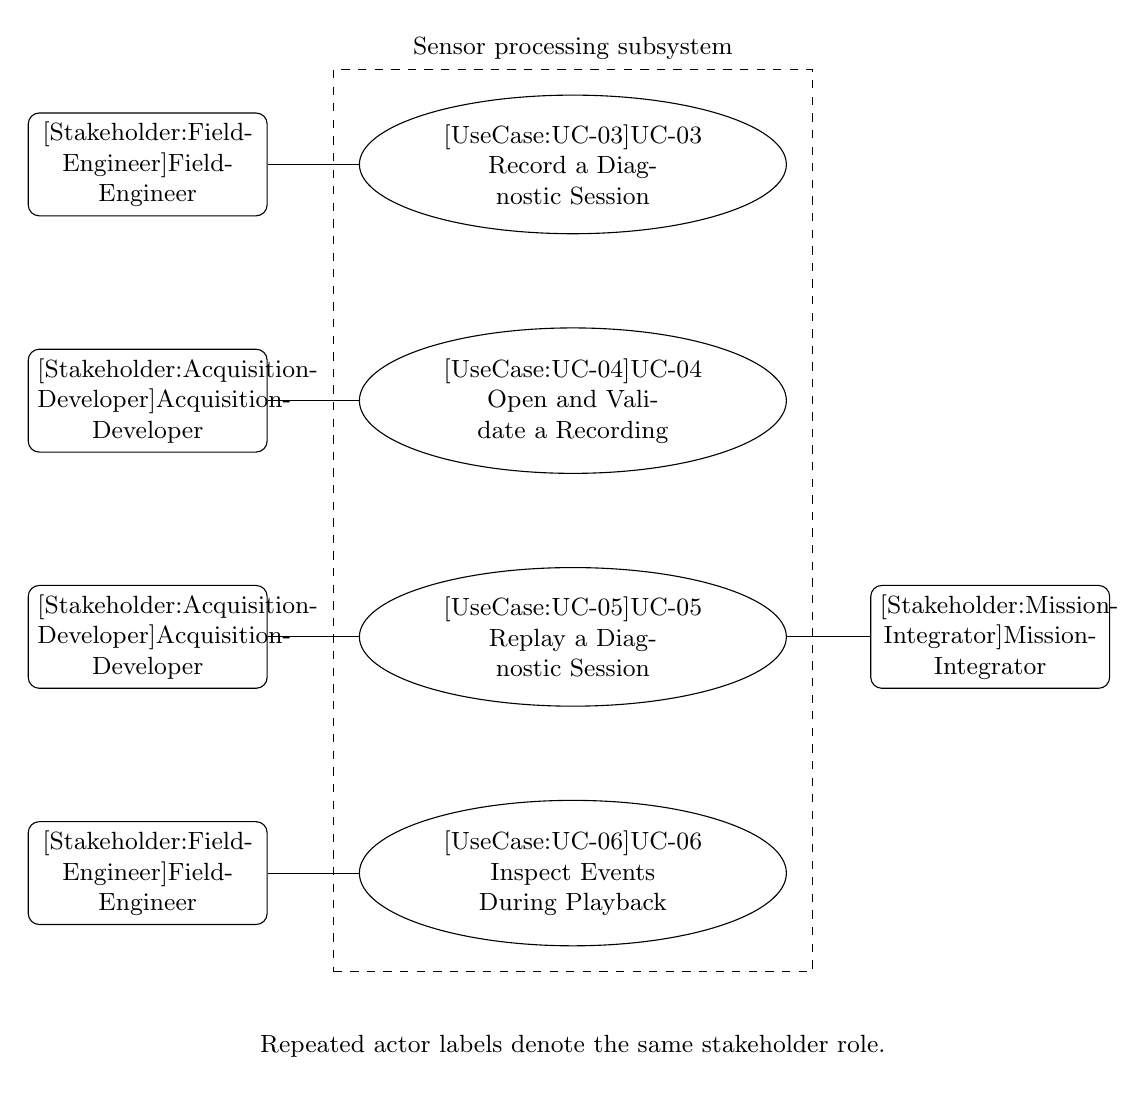
\begin{tikzpicture}[>=Latex,font=\small,
 actor/.style={draw,rounded corners,align=center,text width=2.8cm,minimum height=0.9cm},
 goal/.style={draw,ellipse,align=center,text width=3.6cm,minimum height=1.25cm}]
\node[actor] (field) at (0,0) {\hyperref[Stakeholder:Field-Engineer]{Field-Engineer}};
\node[actor] (devopen) at (0,-3) {\hyperref[Stakeholder:Acquisition-Developer]{Acquisition-Developer}};
\node[actor] (devplay) at (0,-6) {\hyperref[Stakeholder:Acquisition-Developer]{Acquisition-Developer}};
\node[actor] (inspect) at (0,-9) {\hyperref[Stakeholder:Field-Engineer]{Field-Engineer}};
\node[goal] (record) at (5.4,0) {\hyperref[UseCase:UC-03]{UC-03\\Record a Diagnostic Session}};
\node[goal] (open) at (5.4,-3) {\hyperref[UseCase:UC-04]{UC-04\\Open and Validate a Recording}};
\node[goal] (play) at (5.4,-6) {\hyperref[UseCase:UC-05]{UC-05\\Replay a Diagnostic Session}};
\node[goal] (control) at (5.4,-9) {\hyperref[UseCase:UC-06]{UC-06\\Inspect Events During Playback}};
\node[actor] (integrator) at (10.7,-6) {\hyperref[Stakeholder:Mission-Integrator]{Mission-Integrator}};
\node[draw,dashed,fit=(record)(open)(play)(control),inner sep=0.32cm,
 label=above:{Sensor processing subsystem}] {};
\draw (field.east) -- (record.west);
\draw (devopen.east) -- (open.west);
\draw (devplay.east) -- (play.west);
\draw (inspect.east) -- (control.west);
\draw (play.east) -- (integrator.west);
\node[align=center] at (5.4,-11.2) {Repeated actor labels denote the same stakeholder role.};
\end{tikzpicture}
}
\caption{Engineering actors and recording/playback goals at the subsystem boundary.}\label{Figure:DiagnosticUseCases}
\end{figure}

\section{Receive Qualified Sensor Samples}

\small
\begin{tabularx}{\linewidth}{L{2.8cm}Y}
\caption{Receive Qualified Sensor Samples\label{Table:UC-01}\label{Table:SensorUseCase}}\\
\toprule
Field & Candidate scenario\\\midrule
\endfirsthead
\toprule
Field & Candidate scenario\\\midrule
\endhead
\bottomrule
\endlastfoot
ID & \UseCaseID{UC-01}\\
External input & Sensor/FTDI hardware delivers a conversion code and its associated counter value.\\
External recipient & Mission application via OMS.\\
Source stories & \UserStoryRef{US-01}, \UserStoryRef{US-02}, \UserStoryRef{US-04}.\\
Requirements & \RequirementRef{REQ-F-101}, \RequirementRef{REQ-F-102}, \RequirementRef{REQ-F-103}, \RequirementRef{REQ-C-101}, \RequirementRef{REQ-C-102}, \RequirementRef{REQ-C-103}, \RequirementRef{REQ-F-104}, \RequirementRef{REQ-F-105}, \RequirementRef{REQ-F-106}, \RequirementRef{REQ-F-107}, \RequirementRef{REQ-I-101}, \RequirementRef{REQ-SMP-01}, \RequirementRef{REQ-TIM-01}, \RequirementRef{REQ-IF-01}, \RequirementRef{REQ-TIM-02}, \RequirementRef{REQ-F-110}\\
Tests & \TestCaseRef{TC-101}, \TestCaseRef{TC-102}, \TestCaseRef{TC-103}, \TestCaseRef{TC-104}, \TestCaseRef{TC-105}, \TestCaseRef{TC-106}, \TestCaseRef{TC-107}, \TestCaseRef{TC-108}, \TestCaseRef{TC-109}, \TestCaseRef{TC-110}, \TestCaseRef{TC-113}, \TestCaseRef{TC-114}, \TestCaseRef{TC-115}, \TestCaseRef{TC-116}, \TestCaseRef{TC-118}, \TestCaseRef{TC-120}\\
Preconditions & The hardware link, capture rules, qualification rules, and OMS sample contract are configured for the scenario.\\
Trigger & A sample arrives from the Sensor/FTDI hardware.\\
Main flow & The subsystem receives the sample and associated counter value, determines measurement usability, and exposes the local sample record under \RequirementRef{REQ-IF-01}. The Mission application receives the qualified value, status, and timing over OMS. The producer and contract for mission sample delivery are open in \hyperref[Question:Q-118]{Q-118}. The Operator sees the reading attributes at the agreed point of use under \RequirementRef{REQ-F-110}. As earlier samples are processed, acquisition continues as called for by \UserStoryRef{US-02}.\\
Success outcome & The Mission application receives and interprets the qualified sample according to the agreed OMS sample contract.\\
Alternate flow & If a reading is unusable, apply the qualification and publication rules agreed in \hyperref[Question:Q-113]{Q-113} and \hyperref[Question:Q-114]{Q-114}. The disposition remains open.\\
Exceptions & Partial records, loss of input, and delivery failures require agreed handling in \hyperref[Question:Q-107]{Q-107} and \hyperref[Question:Q-114]{Q-114}. Stream cadence and allowable gaps remain open in \hyperref[Question:Q-104]{Q-104}.\\
Postconditions & The Mission application has the sample and its qualification information for the successful transfer.\\
\end{tabularx}
\normalsize

\subsection{Quality Scenarios}
These candidate measures identify what to observe. The linked questions own
the operating limits, expected outputs, and pass thresholds.

\subsubsection{QS-01 Sample integrity and qualification}
\label{Scenario:QS-01}
\begin{description}[leftmargin=0pt,labelindent=0pt,labelsep=0pt,style=nextline]
\item[Stimulus source] Sensor/FTDI hardware driven by reference inputs.
\item[Stimulus] Delivers known conversion-code and counter pairs, including qualification boundary cases.
\item[Environment] Configured acquisition link under nominal operation and qualification boundary conditions.
\item[Artifact] Capture, sample association, qualification, and OMS sample output.
\item[Response] Preserve the sample-to-counter association and publish the value and qualification disposition specified for each reference case.
\item[Response measure] Use the reference vectors to check received values, counter associations, and qualification dispositions. Count mismatches by field and case. Reference inputs and limits are open in \hyperref[Question:Q-108]{Q-108}, \hyperref[Question:Q-112]{Q-112}, and \hyperref[Question:Q-113]{Q-113}.
\end{description}

\subsubsection{QS-02 Acquisition continuity under processing load}
\label{Scenario:QS-02}
\begin{description}[leftmargin=0pt,labelindent=0pt,labelsep=0pt,style=nextline]
\item[Stimulus source] Sensor/FTDI hardware.
\item[Stimulus] Delivers new samples while earlier samples are still being processed.
\item[Environment] Sustained acquisition under the supported processing load.
\item[Artifact] Acquisition, processing, and OMS sample delivery path.
\item[Response] Continue acquiring new samples and deliver the qualified stream to the Mission application.
\item[Response measure] Measure delivered sample rate, maximum gap between deliveries, and count of missing expected samples over the agreed observation interval. Check the 10 ms local publication allocation in \RequirementRef{REQ-TIM-01}. Stream load and delivery limits are open in \hyperref[Question:Q-104]{Q-104}.
\end{description}

\subsubsection{QS-03 Sample freshness}
\label{Scenario:QS-03}
\begin{description}[leftmargin=0pt,labelindent=0pt,labelsep=0pt,style=nextline]
\item[Stimulus source] Sensor/FTDI hardware and the sample processing path.
\item[Stimulus] A sample reaches qualification or delivery after a delay near or beyond the freshness limit.
\item[Environment] Active acquisition with representative processing and delivery delay.
\item[Artifact] Sample timing, qualification, and OMS sample output.
\item[Response] Preserve timing information and apply the agreed freshness disposition so the Mission application can interpret sample age and usability.
\item[Response measure] Measure capture-to-receipt latency and reported or derived age error against reference timestamps. Compare dispositions at the freshness boundary with the agreed examples and check local event timestamp error against the 1 ms allocation in \RequirementRef{REQ-TIM-02}. Timing origin and mission delivery limits are open in \hyperref[Question:Q-104]{Q-104}, \hyperref[Question:Q-113]{Q-113}, and \hyperref[Question:Q-114]{Q-114}.
\end{description}

\subsubsection{QS-04 Sample stream degradation and recovery}
\label{Scenario:QS-04}
\begin{description}[leftmargin=0pt,labelindent=0pt,labelsep=0pt,style=nextline]
\item[Stimulus source] Sensor/FTDI hardware or the OMS delivery path.
\item[Stimulus] Input becomes partial or unavailable, or delivery is interrupted.
\item[Environment] An established sample stream during a fault and subsequent restoration.
\item[Artifact] Acquisition, qualification, and OMS sample delivery path.
\item[Response] Apply the agreed disposition for affected readings and the agreed policy for resuming delivery.
\item[Response measure] Compare affected readings and observable outputs with expected fault outcomes. Measure time from fault onset to observable disposition and from restoration to the first accepted sample, where applicable. Outcomes and limits are open in \hyperref[Question:Q-107]{Q-107} and \hyperref[Question:Q-114]{Q-114}.
\end{description}

\subsubsection{QS-05 Sample interface substitutability}
\label{Scenario:QS-05}
\begin{description}[leftmargin=0pt,labelindent=0pt,labelsep=0pt,style=nextline]
\item[Stimulus source] Mission-Integrator.
\item[Stimulus] Independently replaces the sensor or Mission application with a compatible implementation.
\item[Environment] Integration using the documented sensor-side and OMS sample contracts.
\item[Artifact] Sensor-side sample interface and OMS sample output.
\item[Response] Accept equivalent sensor input or deliver samples the replacement Mission application can interpret using the existing contracts.
\item[Response measure] Run the same sample contract cases before and after each swap. Record field or interpretation mismatches and whether either contract or connection design needed to change. Compatibility criteria are open in \hyperref[Question:Q-102]{Q-102} and \hyperref[Question:Q-114]{Q-114}.
\end{description}

\section{Monitor Sensor Status}

\small
\begin{tabularx}{\linewidth}{L{2.8cm}Y}
\caption{Monitor Sensor Status\label{Table:UC-02}}\\
\toprule
Field & Candidate scenario\\\midrule
\endfirsthead
\toprule
Field & Candidate scenario\\\midrule
\endhead
\bottomrule
\endlastfoot
ID & \UseCaseID{UC-02}\\
Status source & The subsystem uses observed source connection and operating-health information.\\
External recipient & Mission application via OMS.\\
Source stories & \UserStoryRef{US-01} for availability and \UserStoryRef{US-04} for the documented status interface.\\
Requirements & \RequirementRef{REQ-F-108}, \RequirementRef{REQ-F-109}, \RequirementRef{REQ-SMP-02}, \RequirementRef{REQ-OMS-01}\\
Tests & \TestCaseRef{TC-111}, \TestCaseRef{TC-112}, \TestCaseRef{TC-117}, \TestCaseRef{TC-119}\\
Preconditions & Source-health criteria and the OMS status contract are defined for the scenario.\\
Trigger & A source-status observation becomes available for reporting. Reporting cadence and change triggers remain open in \hyperref[Question:Q-114]{Q-114}.\\
Main flow & The subsystem determines source connection and operating-health status from available observations and reports derived status to the Mission application. The mapping from observations to valid, stale, or faulted status remains open in \hyperref[Question:Q-125]{Q-125}.\\
Success outcome & The Mission application can interpret the reported source condition using the agreed OMS status contract.\\
Alternate flow & When observations are stale or insufficient, apply the agreed reporting policy. Status vocabulary and handling remain open in \hyperref[Question:Q-115]{Q-115}.\\
Exceptions & Missing observations and loss of delivery require agreed handling in \hyperref[Question:Q-107]{Q-107} and \hyperref[Question:Q-114]{Q-114}.\\
Postconditions & Source status is available to the Mission application for the successful transfer. The acquisition service exposes stale state and the mission gateway reports derived status under the candidate contracts in \RequirementRef{REQ-SMP-02} and \RequirementRef{REQ-OMS-01}.\\
\end{tabularx}
\normalsize

\subsection{Quality Scenarios}

\subsubsection{QS-06 Status accuracy and delivery timeliness}
\label{Scenario:QS-06}
\begin{description}[leftmargin=0pt,labelindent=0pt,labelsep=0pt,style=nextline]
\item[Stimulus source] Sensor source and connection observations.
\item[Stimulus] A reference fixture produces a known connection transition or operating-health change.
\item[Environment] Monitoring is active and OMS delivery is available.
\item[Artifact] Source-status determination and OMS status output.
\item[Response] Determine the source condition and deliver the corresponding status to the Mission application according to the reporting policy.
\item[Response measure] Compare each delivered state against independent fixture evidence. Measure time from the effective source transition to receipt by the Mission application. Compare CAL messages for valid, stale, and faulted states against the mapping in \RequirementRef{REQ-OMS-01} after program approval. State criteria, reporting cadence, and latency limits are open in \hyperref[Question:Q-114]{Q-114} and \hyperref[Question:Q-115]{Q-115}.
\end{description}

\subsubsection{QS-07 Stale or insufficient status evidence}
\label{Scenario:QS-07}
\begin{description}[leftmargin=0pt,labelindent=0pt,labelsep=0pt,style=nextline]
\item[Stimulus source] Source-status observations.
\item[Stimulus] Observations age past the agreed limit, disappear, or become insufficient to determine source condition.
\item[Environment] Monitoring continues after a previously confirmed state.
\item[Artifact] Status freshness evaluation and OMS status output.
\item[Response] Apply the agreed disposition for stale, missing, or insufficient evidence.
\item[Response measure] Compare the delivered status with the expected fault disposition. Measure elapsed time from the evidence timeout or loss to the observable disposition where applicable. Check the 100 ms local stale-state allocation in \RequirementRef{REQ-SMP-02} separately from OMS delivery. Evidence criteria and reporting policy are open in \hyperref[Question:Q-107]{Q-107}, \hyperref[Question:Q-114]{Q-114}, and \hyperref[Question:Q-115]{Q-115}.
\end{description}

\subsubsection{QS-08 Status delivery interruption and recovery}
\label{Scenario:QS-08}
\begin{description}[leftmargin=0pt,labelindent=0pt,labelsep=0pt,style=nextline]
\item[Stimulus source] OMS delivery path.
\item[Stimulus] Status delivery is interrupted and later becomes available.
\item[Environment] Monitoring remains active while source observations continue.
\item[Artifact] OMS status publication path and Mission application receipt.
\item[Response] Apply the agreed reporting and recovery policy during and after the interruption.
\item[Response measure] Measure the reporting gap and the time from delivery restoration to receipt of the first status allowed by the recovery policy. Compare its state and age with reference observations. Recovery policy and limits are open in \hyperref[Question:Q-107]{Q-107} and \hyperref[Question:Q-114]{Q-114}.
\end{description}

\subsubsection{QS-09 Status interface substitutability}
\label{Scenario:QS-09}
\begin{description}[leftmargin=0pt,labelindent=0pt,labelsep=0pt,style=nextline]
\item[Stimulus source] Mission-Integrator.
\item[Stimulus] Replaces the Mission application with a compatible OMS status consumer.
\item[Environment] Integration using the documented OMS status contract and representative source states.
\item[Artifact] OMS status output and Mission application interpretation.
\item[Response] Deliver status the replacement Mission application can interpret using the existing contract.
\item[Response measure] Run the same status contract cases before and after the swap. Record state, freshness, and interpretation mismatches and whether the contract or connection design needed to change. Compatibility criteria are open in \hyperref[Question:Q-114]{Q-114}.
\end{description}

\begin{figure}[htbp]\centering
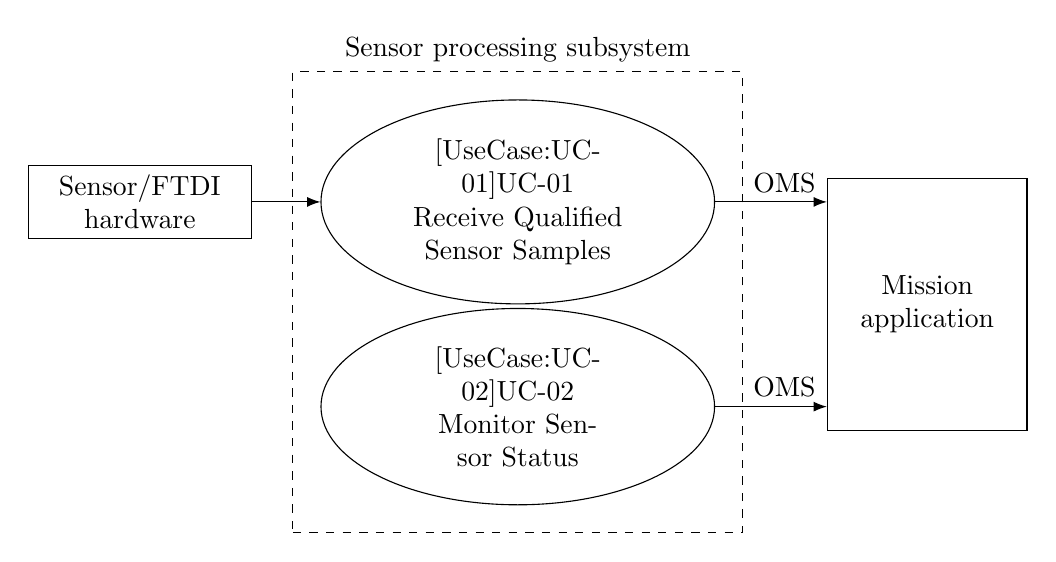
\begin{tikzpicture}[>=Latex]
\node[draw,align=center,text width=2.6cm] (sensor) at (0,1.3)
  {Sensor/FTDI hardware};
\node[draw,ellipse,align=center,text width=3.3cm] (sample) at (4.8,1.3)
  {\hyperref[UseCase:UC-01]{UC-01\\Receive Qualified Sensor Samples}};
\node[draw,ellipse,align=center,text width=3.3cm] (status) at (4.8,-1.3)
  {\hyperref[UseCase:UC-02]{UC-02\\Monitor Sensor Status}};
\node[draw,dashed,fit=(sample)(status),inner sep=0.35cm,
  label=above:{Sensor processing subsystem}] {};
\node[draw,align=center,text width=2.3cm,minimum height=3.2cm] (mission) at (10,0)
  {Mission application};
\draw[->] (sensor.east) -- (sample.west);
\draw[->] (sample.east) -- node[above,pos=0.62]{OMS} (mission.west |- sample.east);
\draw[->] (status.east) -- node[above,pos=0.62]{OMS} (mission.west |- status.east);
\end{tikzpicture}

\caption{Sensor/FTDI input and OMS outputs at the sensor processing subsystem boundary.}\label{Figure:UseCaseDiagram}
\end{figure}

\section{Record a Diagnostic Session}
\par\medskip
\small
\begin{tabularx}{\linewidth}{L{2.8cm}Y}
\caption{Record a Diagnostic Session\label{Table:UC-03}}\\
\toprule
Field & Candidate scenario\\\midrule
\endfirsthead
\toprule
Field & Candidate scenario\\\midrule
\endhead
\bottomrule
\endlastfoot
ID & \UseCaseID{UC-03}\\
Actors & Field-Engineer; Acquisition-Developer supplies reference inputs during verification.\\
Source stories & \UserStoryRef{US-05}, \UserStoryRef{US-08}\\
Requirements & \RequirementRef{REQ-F-111}, \RequirementRef{REQ-F-112}, \RequirementRef{REQ-D-101}, \RequirementRef{REQ-D-102}, \RequirementRef{REQ-F-113}, \RequirementRef{REQ-D-103}, \RequirementRef{REQ-Q-102}, \RequirementRef{REQ-Q-103}, \RequirementRef{REQ-Q-104}, \RequirementRef{REQ-Q-105}\\
Tests & \TestCaseRef{TC-121}, \TestCaseRef{TC-122}, \TestCaseRef{TC-123}, \TestCaseRef{TC-124}, \TestCaseRef{TC-125}, \TestCaseRef{TC-126}, \TestCaseRef{TC-144}, \TestCaseRef{TC-145}, \TestCaseRef{TC-146}, \TestCaseRef{TC-147}\\
Validation & \ValidationRef{VAL-121}\\
Preconditions & The recording boundary, schema, context metadata and fault policy are defined; storage and representative input are available.\\
Trigger & The Field-Engineer requests a diagnostic recording.\\
Main flow & 1. The Field-Engineer starts recording. 2. The subsystem records the observed samples, results and diagnostic events with capture context. 3. Recording continues under the agreed live load. 4. The Field-Engineer requests stop. 5. The subsystem finalizes the recording under the stop-and-flush policy.\\
Success outcome & A readable incident recording retains the agreed capture interval, data associations and context for later investigation.\\
Alternate flow & Known input/recorder gaps are identified; invalid inputs retain the representation defined by the recording schema.\\
Exceptions & Storage is unavailable/full, writes fail, or capture is interrupted. Report failure and preserve recoverable content according to the policy; do not report successful completion for a failed recording.\\
Postconditions & The recording is finalized, or an explicit failure and incomplete-content disposition is available.\\
Open decisions & \hyperref[Question:Q-127]{Q-127}, \hyperref[Question:Q-131]{Q-131}. Other applicable contracts are linked from each requirement.\\
\end{tabularx}
\normalsize
Figure~\ref{Figure:RecordingActivity} shows the recording success and failure paths.
\begin{figure}[htbp]\centering
\resizebox{0.92\linewidth}{!}{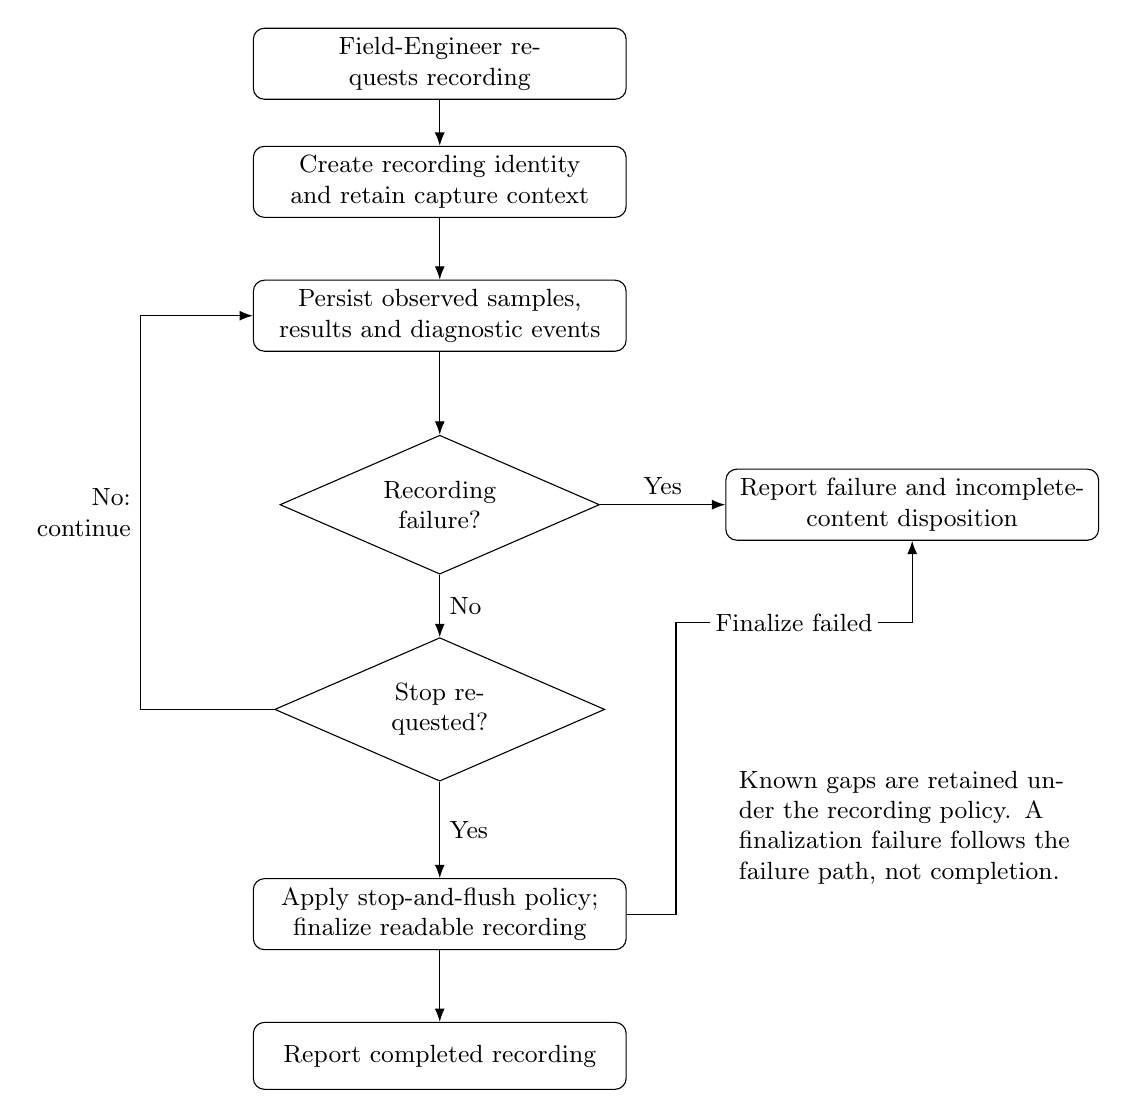
\begin{tikzpicture}[>=Latex,font=\small,
 activity/.style={draw,rounded corners,align=center,text width=4.5cm,minimum height=0.85cm},
 choice/.style={draw,diamond,aspect=2.3,align=center,inner sep=2pt,text width=2.2cm}]
\node[activity] (start) at (0,0) {Field-Engineer requests recording};
\node[activity] (context) at (0,-1.5) {Create recording identity and retain capture context};
\node[activity] (capture) at (0,-3.2) {Persist observed samples, results and diagnostic events};
\node[choice] (fault) at (0,-5.6) {Recording failure?};
\node[choice] (stop) at (0,-8.2) {Stop requested?};
\node[activity] (final) at (0,-10.8) {Apply stop-and-flush policy; finalize readable recording};
\node[activity] (failed) at (6,-5.6) {Report failure and incomplete-content disposition};
\node[activity] (done) at (0,-12.6) {Report completed recording};
\draw[->] (start) -- (context);
\draw[->] (context) -- (capture);
\draw[->] (capture) -- (fault);
\draw[->] (fault) -- node[right]{No} (stop);
\draw[->] (fault.east) -- node[above]{Yes} (failed.west);
\draw[->] (stop) -- node[right]{Yes} (final);
\draw[->] (final) -- (done);
\draw[->] (stop.west) -- (-3.8,-8.2) -- node[left,align=right]{No:\\continue} (-3.8,-3.2) -- (capture.west);
\node[align=left,text width=4.4cm] at (6,-9.7) {Known gaps are retained under the recording policy. A finalization failure follows the failure path, not completion.};
\draw[->] (final.east) -- (3,-10.8) -- (3,-7.1) -- (6,-7.1) -- (failed.south);
\node[fill=white,inner sep=2pt] at (4.5,-7.1) {Finalize failed};
\end{tikzpicture}
}
\caption{Candidate recording activity, including explicit recording failure.}\label{Figure:RecordingActivity}
\end{figure}

\section{Open and Validate a Recording}
\par\medskip
\small
\begin{tabularx}{\linewidth}{L{2.8cm}Y}
\caption{Open and Validate a Recording\label{Table:UC-04}}\\
\toprule
Field & Candidate scenario\\\midrule
\endfirsthead
\toprule
Field & Candidate scenario\\\midrule
\endhead
\bottomrule
\endlastfoot
ID & \UseCaseID{UC-04}\\
Actors & Acquisition-Developer.\\
Source stories & \UserStoryRef{US-06}, \UserStoryRef{US-08}\\
Requirements & \RequirementRef{REQ-F-114}, \RequirementRef{REQ-F-115}, \RequirementRef{REQ-F-116}\\
Tests & \TestCaseRef{TC-127}, \TestCaseRef{TC-128}, \TestCaseRef{TC-129}\\
Validation & \ValidationRef{VAL-122}\\
Preconditions & Compatibility rules, format readers and the context presentation contract are defined; the selected recording is accessible.\\
Trigger & The Acquisition-Developer selects a recorded session.\\
Main flow & 1. Select a recording. 2. The subsystem reads its format and capture context. 3. It evaluates compatibility. 4. The Acquisition-Developer reviews the context and compatibility disposition. 5. A compatible recording becomes ready for playback.\\
Success outcome & The developer understands the capture context and knows whether the recording can be replayed.\\
Alternate flow & Missing metadata or a different software/configuration version receives the disposition specified by the compatibility rules.\\
Exceptions & Unsupported, incompatible, corrupt, truncated, or changed content is classified under the approved rules; playback is prevented when incompatible and the reason is presented.\\
Postconditions & A compatible recording is ready for playback, or an incompatibility disposition is available without admitting recorded input.\\
Open decisions & \hyperref[Question:Q-128]{Q-128}, \hyperref[Question:Q-131]{Q-131}. Other applicable contracts are linked from each requirement.\\
\end{tabularx}
\normalsize

\section{Replay a Diagnostic Session}
\par\medskip
\small
\begin{tabularx}{\linewidth}{L{2.8cm}Y}
\caption{Replay a Diagnostic Session\label{Table:UC-05}}\\
\toprule
Field & Candidate scenario\\\midrule
\endfirsthead
\toprule
Field & Candidate scenario\\\midrule
\endhead
\bottomrule
\endlastfoot
ID & \UseCaseID{UC-05}\\
Actors & Acquisition-Developer; Mission-Integrator observes the selected output consumer.\\
Source stories & \UserStoryRef{US-06}, \UserStoryRef{US-09}\\
Requirements & \RequirementRef{REQ-F-117}, \RequirementRef{REQ-F-127}, \RequirementRef{REQ-D-104}, \RequirementRef{REQ-Q-101}, \RequirementRef{REQ-I-102}, \RequirementRef{REQ-I-103}, \RequirementRef{REQ-F-126}\\
Tests & \TestCaseRef{TC-130}, \TestCaseRef{TC-149}, \TestCaseRef{TC-131}, \TestCaseRef{TC-132}, \TestCaseRef{TC-141}, \TestCaseRef{TC-142}, \TestCaseRef{TC-143}\\
Validation & \ValidationRef{VAL-123}\\
Preconditions & The recording has passed the compatibility gate; input boundary, time/order rules, replay identification and output routing contracts are defined; an allowed endpoint is selected.\\
Trigger & The Acquisition-Developer requests playback of a compatible recording.\\
Main flow & 1. Start playback without Sensor/FTDI hardware and establish the approved initial processing state before admitting the first event. 2. The subsystem admits recorded events in their defined order and timing. 3. The processing path produces results. 4. The consumer and engineer receive explicitly identified replay outputs at the selected endpoint. 5. At end of recording, completion is reported.\\
Success outcome & The developer can investigate the captured software behavior and the Mission-Integrator can distinguish recorded measurements from current live measurements.\\
Alternate flow & Recorded gaps and disconnect events are replayed as defined by the captured event schema; playback can be inspected through \UseCaseRef{UC-06}.\\
Exceptions & Unavailable initial processing state receives the approved disposition without admitting recorded input. Read, processing or delivery failure follows the defined lifecycle/routing disposition. Missing endpoint selection does not silently select a mission endpoint.\\
Postconditions & The last processed position and completion/failure state are available; outputs have followed the approved replay-identification and routing rules.\\
Open decisions & \hyperref[Question:Q-129]{Q-129}, \hyperref[Question:Q-131]{Q-131}. Other applicable contracts are linked from each requirement.\\
\end{tabularx}
\normalsize
Figure~\ref{Figure:PlaybackSequence} shows externally meaningful playback interactions. Subsystem lanes denote behavior, not selected processes, threads or classes. See \hyperref[Question:Q-129]{Q-129} and \hyperref[Question:Q-130]{Q-130} for the input and routing contracts.
\begin{figure}[htbp]\centering
\resizebox{0.98\linewidth}{!}{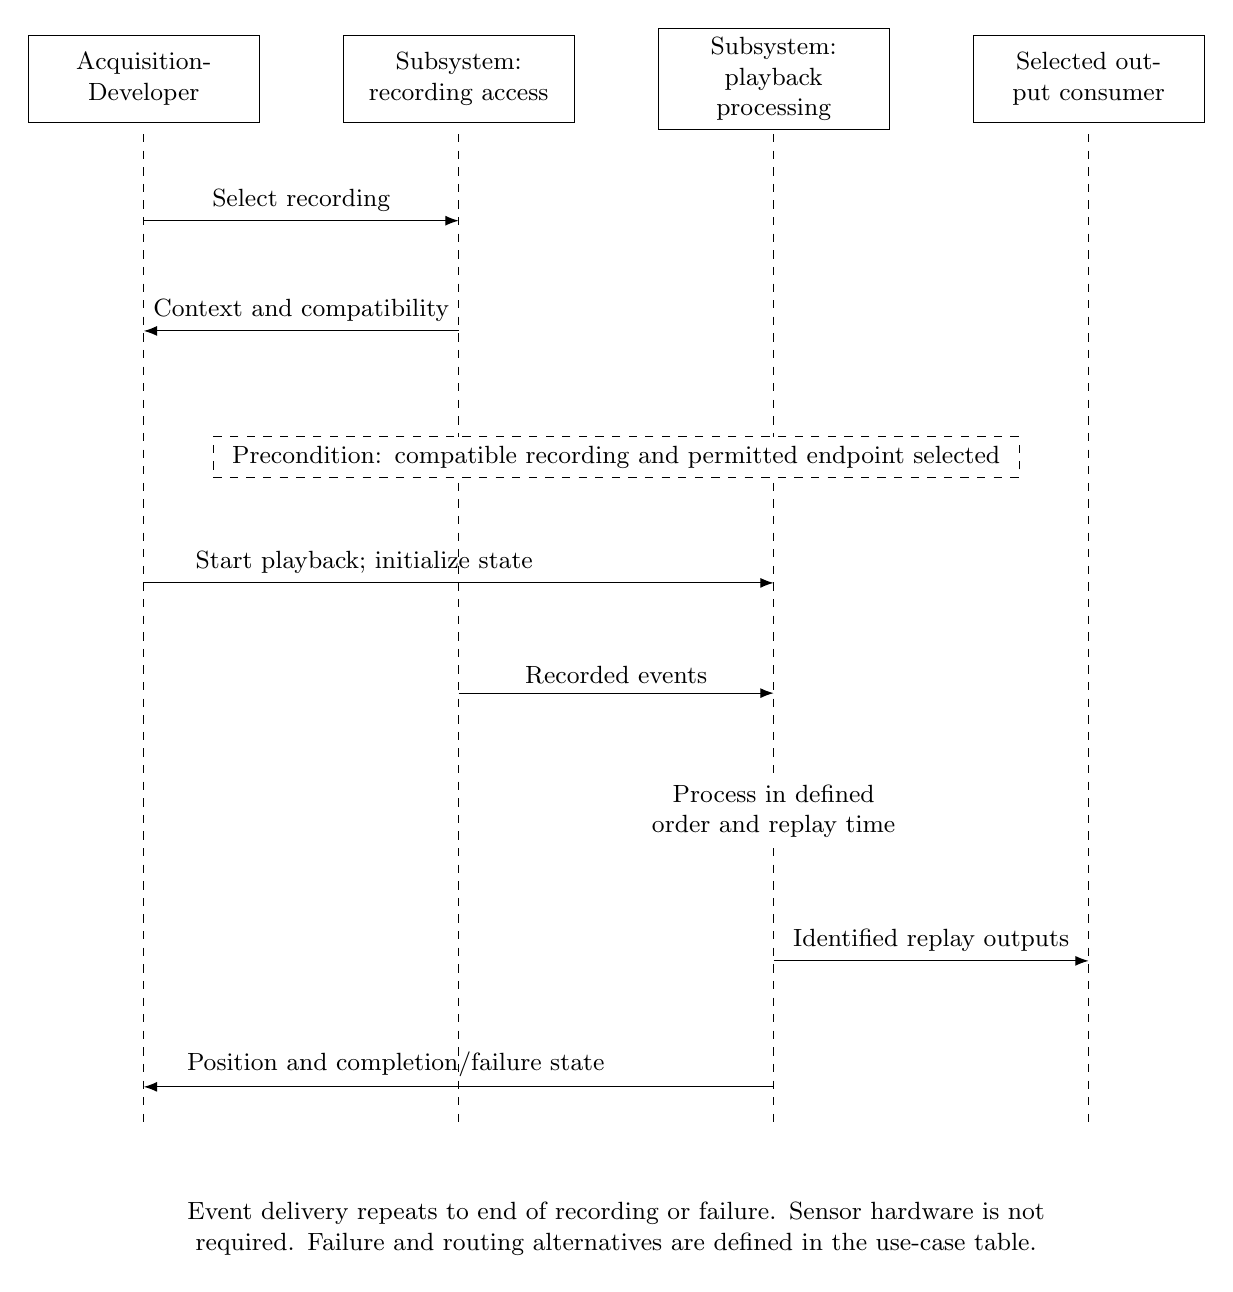
\begin{tikzpicture}[>=Latex,font=\small,
 lane/.style={draw,align=center,text width=2.7cm,minimum height=1.1cm}]
\node[lane] (user) at (0,0) {Acquisition-Developer};
\node[lane] (session) at (4,0) {Subsystem:\\recording access};
\node[lane] (process) at (8,0) {Subsystem:\\playback processing};
\node[lane] (consumer) at (12,0) {Selected output consumer};
\foreach \x in {0,4,8,12} {\draw[dashed] (\x,-0.7) -- (\x,-13.3);}
\draw[->] (0,-1.8) -- node[above]{Select recording} (4,-1.8);
\draw[->] (4,-3.2) -- node[above]{Context and compatibility} (0,-3.2);
\node[draw,dashed,align=center,fill=white,text width=10cm] at (6,-4.8)
 {Precondition: compatible recording and permitted endpoint selected};
\draw[->] (0,-6.4) -- node[above,pos=0.35]{Start playback; initialize state} (8,-6.4);
\draw[->] (4,-7.8) -- node[above]{Recorded events} (8,-7.8);
\node[align=center,text width=3.6cm,fill=white] at (8,-9.3) {Process in defined order and replay time};
\draw[->] (8,-11.2) -- node[above]{Identified replay outputs} (12,-11.2);
\draw[->] (8,-12.8) -- node[above,pos=0.6]{Position and completion/failure state} (0,-12.8);
\node[align=center,text width=11cm] at (6,-14.6)
 {Event delivery repeats to end of recording or failure. Sensor hardware is not required. Failure and routing alternatives are defined in the use-case table.};
\end{tikzpicture}
}
\caption{Candidate playback interaction after compatibility and endpoint selection.}\label{Figure:PlaybackSequence}
\end{figure}

\section{Inspect Events During Playback}
\par\medskip
\small
\begin{tabularx}{\linewidth}{L{2.8cm}Y}
\caption{Inspect Events During Playback\label{Table:UC-06}}\\
\toprule
Field & Candidate scenario\\\midrule
\endfirsthead
\toprule
Field & Candidate scenario\\\midrule
\endhead
\bottomrule
\endlastfoot
ID & \UseCaseID{UC-06}\\
Actors & Field-Engineer.\\
Source stories & \UserStoryRef{US-07}\\
Requirements & \RequirementRef{REQ-F-118}, \RequirementRef{REQ-F-119}, \RequirementRef{REQ-F-120}, \RequirementRef{REQ-F-121}, \RequirementRef{REQ-F-122}, \RequirementRef{REQ-F-123}, \RequirementRef{REQ-F-124}, \RequirementRef{REQ-F-125}, \RequirementRef{REQ-Q-106}\\
Tests & \TestCaseRef{TC-133}, \TestCaseRef{TC-134}, \TestCaseRef{TC-135}, \TestCaseRef{TC-136}, \TestCaseRef{TC-137}, \TestCaseRef{TC-138}, \TestCaseRef{TC-139}, \TestCaseRef{TC-140}, \TestCaseRef{TC-148}\\
Validation & \ValidationRef{VAL-124}\\
Preconditions & A compatible recording is open; supported controls, playback states, replay-clock and state-restoration policies are defined.\\
Trigger & The Field-Engineer requests a playback control action while investigating an incident.\\
Main flow & 1. Locate the incident position. 2. Pause and inspect the selected record and status. 3. Step through individual events. 4. Seek backward or forward with the defined state restoration. 5. Change speed or resume and inspect the event sequence.\\
Success outcome & The engineer can examine the events surrounding a fault with interpretable position, state and timing information.\\
Alternate flow & A seek restores the approved state before further event admission; pausing and speed changes apply the replay-clock policy to freshness and timeouts.\\
Exceptions & Invalid locations, unsupported speeds and controls issued in an invalid state receive the approved disposition. End-of-recording and processing errors follow the playback lifecycle policy.\\
Postconditions & Playback position and state correspond to the last accepted action, with restored processing state where required.\\
Open decisions & \hyperref[Question:Q-129]{Q-129}, \hyperref[Question:Q-131]{Q-131}. Other applicable contracts are linked from each requirement.\\
\end{tabularx}
\normalsize
Figure~\ref{Figure:PlaybackStates} illustrates the candidate observable states. Ready follows successful compatibility evaluation; Playing admits events, Paused permits inspection and single-step, Completed indicates end of recording, and Error indicates failed playback. Seeking and speed selection apply the policy in \hyperref[Question:Q-129]{Q-129}; the diagram does not select an internal state-machine implementation.
\begin{figure}[htbp]\centering
\resizebox{0.96\linewidth}{!}{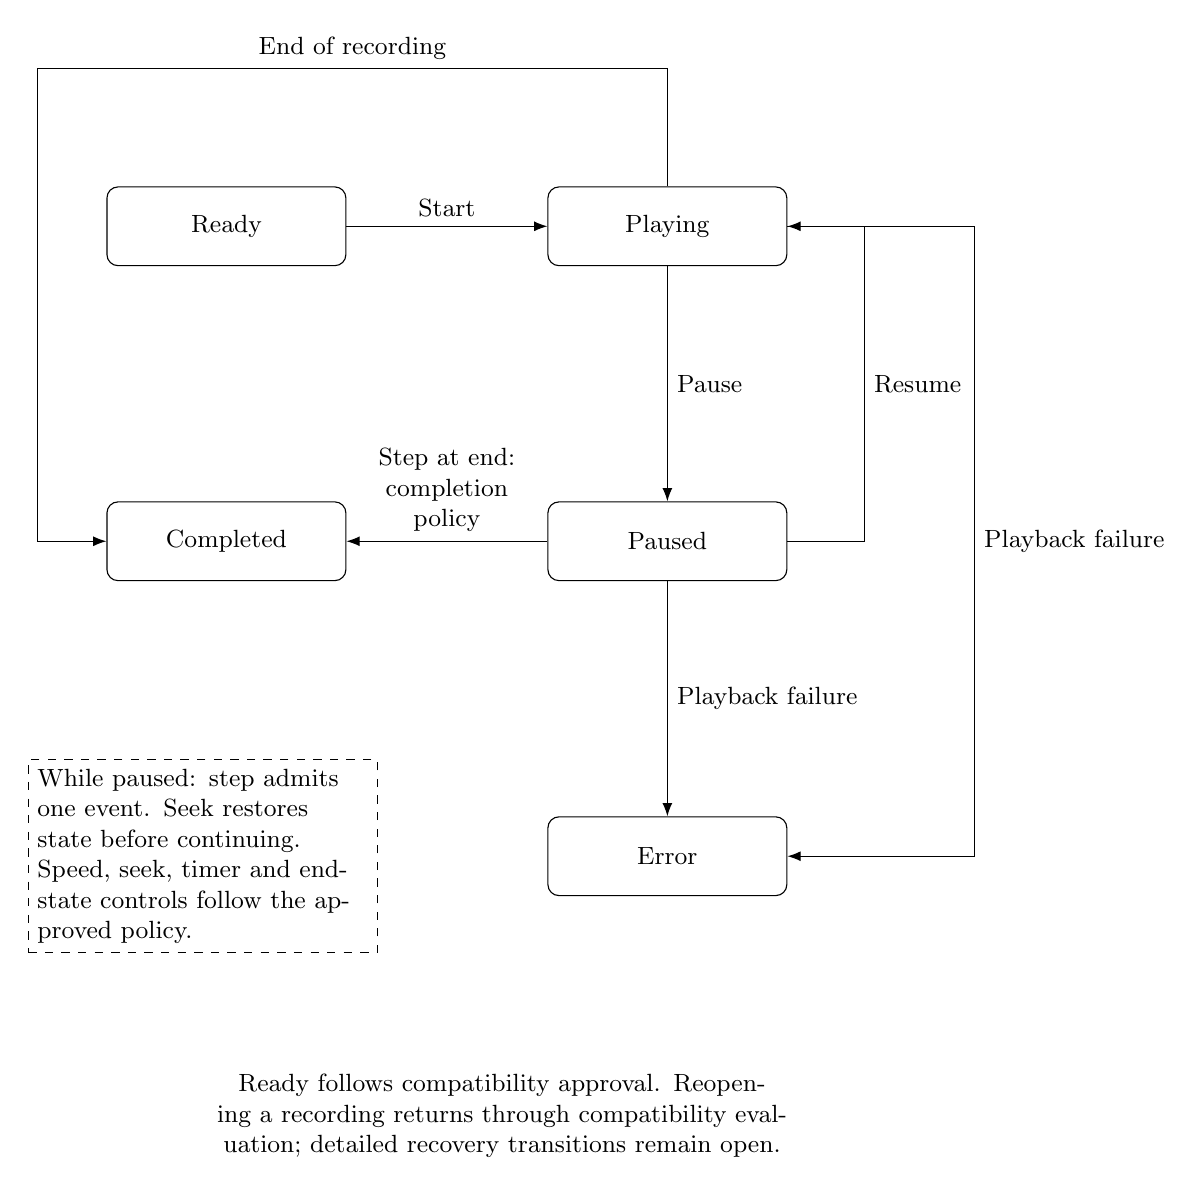
\begin{tikzpicture}[>=Latex,font=\small,
 state/.style={draw,rounded corners,align=center,text width=2.8cm,minimum height=1cm}]
\node[state] (ready) at (0,0) {Ready};
\node[state] (playing) at (5.6,0) {Playing};
\node[state] (paused) at (5.6,-4) {Paused};
\node[state] (completed) at (0,-4) {Completed};
\node[state] (error) at (5.6,-8) {Error};
\draw[->] (ready.east) -- node[above]{Start} (playing.west);
\draw[->] (playing.south) -- node[right]{Pause} (paused.north);
\draw[->] (paused.east) -- (8.1,-4) -- node[right]{Resume} (8.1,0) -- (playing.east);
\draw[->] (playing.north) -- (5.6,2) -- node[above]{End of recording} (-2.4,2) -- (-2.4,-4) -- (completed.west);
\draw[->] (paused.west) -- node[above,align=center,text width=2.4cm]{Step at end:\\completion policy} (completed.east);
\draw[->] (paused.south) -- node[right]{Playback failure} (error.north);
\draw[->] (playing.east) -- (9.5,0) -- node[right]{Playback failure} (9.5,-8) -- (error.east);
\node[draw,dashed,align=left,text width=4.2cm] at (-0.3,-8)
 {While paused: step admits one event. Seek restores state before continuing. Speed, seek, timer and end-state controls follow the approved policy.};
\node[align=center,text width=10cm] at (3.5,-11.3)
 {Ready follows compatibility approval. Reopening a recording returns through compatibility evaluation; detailed recovery transitions remain open.};
\end{tikzpicture}
}
\caption{Candidate playback states and stakeholder control transitions.}\label{Figure:PlaybackStates}
\end{figure}

\chapter{Architecture Overview}
\ChapterLabel{ArchitectureOverview}
\label{Section:ArchitectureOverviewResponsibility}
This chapter records the selected measurement path and the unresolved design decisions.


\section{Software Direction}
\ArchitectureID{ARC-101}: Retain C++ for the control app and the previously scoped embedded software (\RequirementRef{REQ-C-101}, \RequirementRef{REQ-C-102}). The host executes on macOS (\RequirementRef{REQ-C-103}). C++ is a user-selected constraint, not the outcome of a language trade study. The embedded execution allocation and toolchains remain \hyperref[Question:Q-106]{Q-106}, \hyperref[Question:Q-116]{Q-116}. A FIFO interface IC does not by itself establish an embedded processor or firmware target.

\section{Refined Boundary}
\ArchitectureID{ARC-102}: The earlier two-application sensor-to-host boundary is refined to the complete measurement path and downstream publication boundary in Figure~\ref{Figure:SensorContext}. Drivers and reciprocal mappings are maintained in \hyperref[Table:TraceabilityMatrix]{the traceability register}. The previous boundary is not an additional competing architecture; its selected component allocation is defined by \ArchitectureRef{ARC-103} and \ArchitectureRef{ARC-104}.

\section{Acquisition and Transfer Allocation}
\ArchitectureID{ARC-103}: Use the user-selected sensor/ADC0804 conversion path, clock/counter, interface logic, FT245R USB-to-parallel data path, and macOS host. Drivers: \RequirementRef{REQ-F-101}, \RequirementRef{REQ-F-102}, \RequirementRef{REQ-F-103}, \RequirementRef{REQ-F-104}, \RequirementRef{REQ-F-105}, \RequirementRef{REQ-C-103}. The conversion code is 8-bit; counter width and time meaning remain \hyperref[Question:Q-111]{Q-111}. The two logical inputs meet in interface logic; the diagram is not a direct-wiring instruction. Capturing/latching both inputs before serialization, or another explicitly coherent acquisition method, are alternatives to evaluate against capture skew, clock domains, rollover, and backpressure. None is selected. FT245R bus ownership, framing, and capture association remain \hyperref[Question:Q-103]{Q-103}, \hyperref[Question:Q-112]{Q-112}. Consequence: a received code is not automatically associated with the correct measurement time.

\section{Qualification and Result Publication}
\ArchitectureID{ARC-104}: Allocate qualification of measurement usability and publication of code, status, and timing to the macOS control app. Allocate connection and operating-health information to support the Field-Engineer need. Drivers: \RequirementRef{REQ-F-106}, \RequirementRef{REQ-F-107}, \RequirementRef{REQ-F-108}, \RequirementRef{REQ-F-109}, \RequirementRef{REQ-I-101}. The downstream consumer is external; the result contract is the integration boundary. Qualification rules, published-code meaning, timing provenance, result transport, and diagnostic coverage remain \hyperref[Question:Q-113]{Q-113}, \hyperref[Question:Q-114]{Q-114}, \hyperref[Question:Q-115]{Q-115}. A local function/API, stream, file, or network endpoint are alternatives for publication, not selected interfaces. The proposed operator-facing presentation obligation is \RequirementRef{REQ-F-110}. Its endpoint, age semantics, and presentation contract are open in \hyperref[Question:Q-119]{Q-119}.


\paragraph{Candidate acquisition service and mission gateway boundaries}
\ArchitectureID{ARC-105}. The acquisition service publishes the local
sample record to the local downstream consumer. The mission gateway
publishes the derived sensor-status product at the program-approved OMS
CAL boundary. Drivers include \RequirementRef{REQ-SMP-01},
\RequirementRef{REQ-TIM-01}, \RequirementRef{REQ-IF-01},
\RequirementRef{REQ-SMP-02}, \RequirementRef{REQ-TIM-02}, and
\RequirementRef{REQ-OMS-01}. See
\hyperref[Table:SampleExchangeBoundaries]{the interface decisions} for the
open contracts and allocations.

\chapter{User Interface Design}
\ChapterLabel{UserInterfaceDesign}
\section{Chapter Responsibility}
\label{Section:UserInterfaceDesignResponsibility}
Record Operator and Maintainer interaction needs without choosing a screen or command interface.

\noindent\textbf{Expected result:} Interaction needs for the Operator and Maintainer, with UI mechanism undecided.

\section{Stakeholder Interaction Needs}
The \hyperref[Stakeholder:Operator]{Operator} needs the decision about measurement usability (\UserStoryRef{US-101}). The \hyperref[Stakeholder:Maintainer]{Maintainer} needs connection and operating-health information (\UserStoryRef{US-103}). The \hyperref[Stakeholder:Integrator]{Integrator} needs the semantics and format of the downstream result (\UserStoryRef{US-102}); that integration boundary is not necessarily a human UI.

Qualification and result publication are supported by \RequirementRef{REQ-F-106} and \RequirementRef{REQ-F-107}. Connection and operating-health information are supported by \RequirementRef{REQ-F-108} and \RequirementRef{REQ-F-109}. No GUI, command-line syntax, polling cadence, indicator colors, status enumeration, or control channel is selected. Human presentation/access and stale/unknown/error behavior remain \hyperref[Question:Q-105]{Q-105}, \hyperref[Question:Q-113]{Q-113}, \hyperref[Question:Q-114]{Q-114}, \hyperref[Question:Q-115]{Q-115}. Future wireframes and accessibility criteria depend on those choices.

\chapter{Logical View}
\ChapterLabel{LogicalView}
\label{Section:LogicalViewResponsibility}
This chapter defines conceptual responsibilities and data boundaries without selecting C++ classes.


\section{Responsibility and Contract Map}
These are conceptual responsibilities, not implemented classes. The register identifies their inputs, outputs, and governing requirements. No class diagram or C++ API is selected.

\small
\begin{tabularx}{\linewidth}{L{3.0cm}Y}
\caption{Measurement Responsibilities\label{Table:MeasurementResponsibilities}}\\
\toprule
Responsibility & Inputs, outputs, and governing links\\\midrule
\endfirsthead
\toprule
Responsibility & Inputs, outputs, and governing links\\\midrule
\endhead
\bottomrule
\endlastfoot
Analog conversion & \RequirementRef{REQ-F-101}; sensor signal to ADC0804 8-bit conversion code. Analog span/reference/calibration: \hyperref[Question:Q-102]{Q-102}.\\
Counter observation & \RequirementRef{REQ-F-104}; clock/counter to counter value. Width, event and rollover: \hyperref[Question:Q-111]{Q-111}.\\
Capture and association & \RequirementRef{REQ-F-105}; conversion and counter inputs to an associated acquisition record. No record layout is selected: \hyperref[Question:Q-112]{Q-112}.\\
FT245R transfer and host reception & \RequirementRef{REQ-F-102}, \RequirementRef{REQ-F-103}; associated acquisition data across parallel/USB boundaries. Framing and partial records: \hyperref[Question:Q-103]{Q-103}.\\
Qualification & \RequirementRef{REQ-F-106}; received measurement evidence to a usability disposition under \hyperref[Question:Q-113]{Q-113}.\\
Publication & \RequirementRef{REQ-F-107}, \RequirementRef{REQ-I-101}; code, status, timing to downstream consumer under \hyperref[Question:Q-114]{Q-114}.\\
Source condition & \RequirementRef{REQ-F-108}, \RequirementRef{REQ-F-109}; defined observations to Field-Engineer connection/health information under \hyperref[Question:Q-115]{Q-115}.\\
iOS presentation & \RequirementRef{REQ-C-104}, \RequirementRef{REQ-F-110}; processing-core reading and status outputs to the iOS SwiftUI UI. The UI/core contract remains \hyperref[Question:Q-106]{Q-106}; presentation semantics remain \hyperref[Question:Q-105]{Q-105}.\\
\end{tabularx}
\normalsize

\section{Data Meaning and Invariants Awaiting Definition}
\label{Section:DataMeaning}
Conversion code, counter value, host qualification status, and published code are separate terms. The published code is not assumed to be the raw conversion code. Counter value is not assumed to be elapsed time, absolute time, or the host receive timestamp. A record's association, timing origin, field units, lifecycle, and representation are defined only after \hyperref[Question:Q-111]{Q-111}, \hyperref[Question:Q-112]{Q-112}, \hyperref[Question:Q-114]{Q-114} is resolved. No packed structure, byte order, checksum, or wall-clock mapping is introduced here.

\chapter{Runtime Behavior}
\ChapterLabel{ProcessView}
\label{Section:ProcessViewResponsibility}
This chapter describes conversion, association, qualification, and publication while exposing timing/fault gaps.


\section{Measurement Flow}
The high-level flow is \UseCaseRef{UC-01}: conversion code and clock/counter value become available; interface logic captures and associates them, transfers the acquisition record through FT245R USB, and the macOS host receives, qualifies, and publishes the result. Figure~\ref{Figure:SensorContext} shows this direction; \ArchitectureRef{ARC-103} and \ArchitectureRef{ARC-104} define the allocation.

The word alongside does not guarantee simultaneous sampling or coherent capture. Conversion completion, counter transition/rollover, serialization, USB delivery, host qualification, and publication are different events. Their ordering, deadlines, latency, clock relationships, and timestamps remain \hyperref[Question:Q-103]{Q-103}, \hyperref[Question:Q-104]{Q-104}, \hyperref[Question:Q-111]{Q-111}, \hyperref[Question:Q-112]{Q-112}. No thread, queue, scheduling, or state-machine structure is selected.

\section{Fault and Maintenance Paths}
\UseCaseRef{UC-02} addresses source connection and operating health independently of measurement qualification. A connection can exist without demonstrated operation, and a received record does not by itself prove measurement usability. The required evidence, stale/unknown behavior, fault detection, recovery, and publication policy remain \hyperref[Question:Q-107]{Q-107}, \hyperref[Question:Q-113]{Q-113}, \hyperref[Question:Q-114]{Q-114}, \hyperref[Question:Q-115]{Q-115}. A complete state model and exception transition table depend on those decisions; this revision does not invent fail-safe or suppression behavior.

\chapter{Development View}
\ChapterLabel{DevelopmentView}
\label{Section:DevelopmentViewResponsibility}
This chapter describes the planned software organization and unresolved build and dependency boundaries.



\section{Future Application Organization}
The embedded C++ allocation and control-app C++ processing core follow \RequirementRef{REQ-C-101} and \RequirementRef{REQ-C-102}. The control app targets macOS, Windows 11, and iOS under \RequirementRef{REQ-C-103}; its iOS UI uses SwiftUI under \RequirementRef{REQ-C-104}. A shared C++ core with platform connection/lifecycle adapters and an iOS SwiftUI presentation layer is the proposed organization in \ArchitectureRef{ARC-101}. Library/module boundaries, the SwiftUI-to-C++ interface, repository layout, dependency rules, CI, packaging and adapter implementations remain unselected. Plan separate build and validation coverage for all three platforms, including device execution and UI/core integration on iOS. Interface logic is not assumed to be an embedded C++ module; its allocation remains \hyperref[Question:Q-116]{Q-116}. Decisions depend on \hyperref[Question:Q-102]{Q-102}, \hyperref[Question:Q-103]{Q-103}, \hyperref[Question:Q-106]{Q-106}. No application code or build instructions are asserted by this documentation stage.

\chapter{Physical View}
\ChapterLabel{PhysicalView}
\section{Chapter Responsibility}
\label{Section:PhysicalViewResponsibility}
Describe the chosen hardware path, macOS host, and external downstream boundary.

\noindent\textbf{Expected result:} A deployment view of the selected devices and macOS host.

\section{Selected Components and Deployment}
Figure~\ref{Figure:SensorContext} shows the sensor coupled to ADC0804, a clock/counter, interface logic, FT245R, and a macOS host. The first two digital outputs are logical inputs to the interface logic; the FT245R path connects the resulting transfers to USB at the host. The downstream consumer remains outside the system of interest. See \ArchitectureRef{ARC-103} and \ArchitectureRef{ARC-104}.

Sensor characteristics, ADC0804 manufacturer/grade/board revision, conversion reference/clock, counter hardware, supply/logic levels, bus ownership, and a controlled schematic remain \hyperref[Question:Q-102]{Q-102}, \hyperref[Question:Q-103]{Q-103}, \hyperref[Question:Q-111]{Q-111}, \hyperref[Question:Q-112]{Q-112}. The FT245R selection does not select a development module, substitute FT245RN device, driver API, firmware target, or programmable-logic implementation. Software execution allocation remains \hyperref[Question:Q-116]{Q-116}.

Only macOS is in the current host scope; supported versions and processor architectures, USB permissions/driver, packaging, and downstream placement/transport remain \hyperref[Question:Q-106]{Q-106}, \hyperref[Question:Q-114]{Q-114}. Hardware electrical/timing compatibility and operation have not been demonstrated.

\chapter{Implementation Constraints}
\ChapterLabel{Implementation}
\label{Section:ImplementationResponsibility}
This chapter records implementation constraints, allocation limits, and the absence of a product baseline.



\section{Application Baseline}
The macOS control app and previously scoped embedded software use C++ (\RequirementRef{REQ-C-101}, \RequirementRef{REQ-C-102}; rationale in \ArchitectureRef{ARC-101}). No C++ standard, compiler, SDK, RTOS, host toolkit, library, application build command, or implementation version is selected. See \hyperref[Question:Q-106]{Q-106} and the unresolved embedded allocation in \hyperref[Question:Q-116]{Q-116}. This stage contains no application implementation or executed product tests.

\chapter{Tests}
\ChapterLabel{Tests}
\section{Chapter Responsibility}
\label{Section:TestsResponsibility}
Define planned tests for the measurement path, qualification, publication, and source condition.

\noindent\textbf{Expected result:} Linked procedures and expected outcomes that remain distinguishable from results.

\section{Candidate Test Definitions}
All product tests are Not Executed. Michael Stoddard owns verification/validation planning. Entry requires an accepted candidate requirement, controlled implementation/hardware revision, resolved referenced contracts, calibrated/known fixtures, and approved expected data. Every execution must retain input, configuration, command/procedure, expected and observed result, hardware/platform/tool versions, date, operator, and evidence path. The definitions below are blocked test outlines until their owned prerequisites are answered, not completed repeatable test specifications. Interface and fault fixtures require \hyperref[Question:Q-108]{Q-108}.

\small
\begin{tabularx}{\linewidth}{L{2cm}Y}
\caption{Planned Test Cases\label{Table:ProjectTests}}\\
\toprule
ID & Mappings, procedure, and expected result\\\midrule
\endfirsthead
\toprule
ID & Mappings, procedure, and expected result\\\midrule
\endhead
\bottomrule
\endlastfoot
\TestCaseID{TC-101} & \RequirementRef{REQ-F-101}; \UseCaseRef{UC-101}. Procedure: Apply approved reference sensor inputs and capture the ADC0804 conversion code at the acquisition boundary. Compare to the approved reference values. Expected result: An 8-bit code is acquired with the approved analog span, reference, calibration, timing, and tolerance; these parameters require \hyperref[Question:Q-102]{Q-102}, \hyperref[Question:Q-104]{Q-104}, \hyperref[Question:Q-108]{Q-108}. Actual result: not executed; no product evidence available.\\
\TestCaseID{TC-102} & \RequirementRef{REQ-F-102}; \UseCaseRef{UC-101}. Procedure: Transfer an approved sequence through the selected interface logic and FT245R. Compare the captured USB receive stream with the reference sequence. Expected result: The transfer preserves the agreed record content under the approved framing, ordering, and backpressure contract in \hyperref[Question:Q-103]{Q-103}, \hyperref[Question:Q-112]{Q-112}. Actual result: not executed; no product evidence available.\\
\TestCaseID{TC-103} & \RequirementRef{REQ-F-103}; \UseCaseRef{UC-101}. Procedure: Supply an approved sequence of conversion/counter associations through the FT245R path and inspect the host receive boundary. Expected result: Host receive records match the expected associations under \hyperref[Question:Q-103]{Q-103}, \hyperref[Question:Q-111]{Q-111}, \hyperref[Question:Q-112]{Q-112}, \hyperref[Question:Q-108]{Q-108}. Actual result: not executed; no product evidence available.\\
\TestCaseID{TC-104} & \RequirementRef{REQ-C-101}; \UseCaseRef{UC-101}. Procedure: Once the execution allocation is accepted, inspect the embedded software source and configuration and build it with the selected target C++ toolchain. Expected result: The allocated embedded software is C++ and builds with the approved configuration. This test is blocked until \hyperref[Question:Q-106]{Q-106}, \hyperref[Question:Q-116]{Q-116}; it does not assume that interface logic is firmware. Actual result: not executed; no product evidence available.\\
\TestCaseID{TC-105} & \RequirementRef{REQ-C-102}; \UseCaseRef{UC-101}. Procedure: Inspect the control-app source inventory and build configuration, then build with the approved macOS C++ toolchain. Expected result: The control app is C++ and builds with the approved toolchain in \hyperref[Question:Q-106]{Q-106}. Actual result: not executed; no product evidence available.\\
\TestCaseID{TC-106} & \RequirementRef{REQ-C-103}; \UseCaseRef{UC-101}. Procedure: Build and run the measurement scenario on every approved macOS/version/architecture combination and retain the per-platform results. Expected result: Each approved macOS configuration runs the scenario; versions, architectures, drivers, and fixture criteria require \hyperref[Question:Q-106]{Q-106}, \hyperref[Question:Q-108]{Q-108}. Actual result: not executed; no product evidence available.\\
\TestCaseID{TC-107} & \RequirementRef{REQ-F-104}; \UseCaseRef{UC-101}. Procedure: Drive an approved reference clock/counter sequence and conversion input. Capture the counter value delivered alongside each code, including rollover cases. Expected result: Observed counter values agree with the approved event, width, rate, reset, and rollover definitions in \hyperref[Question:Q-111]{Q-111}, \hyperref[Question:Q-112]{Q-112}. Actual result: not executed; no product evidence available.\\
\TestCaseID{TC-108} & \RequirementRef{REQ-F-105}; \UseCaseRef{UC-101}. Procedure: Exercise conversion and counter transitions around the approved capture event, including delayed transitions and backpressure. Inspect capture associations and the serialized transfer. Expected result: Every association follows the approved capture/coherence/association rule, including specified exceptional cases; the rule and fixture timing require \hyperref[Question:Q-112]{Q-112}, \hyperref[Question:Q-103]{Q-103}, \hyperref[Question:Q-108]{Q-108}. Actual result: not executed; no product evidence available.\\
\TestCaseID{TC-109} & \RequirementRef{REQ-F-106}; \UseCaseRef{UC-101}. Procedure: Apply approved usable, unusable, and boundary-case input vectors with expected dispositions to the host qualifier. Compare every observed disposition with its reference. Expected result: The qualification decision matches the approved rules and expected results in \hyperref[Question:Q-113]{Q-113}; no threshold or status enumeration is yet selected. Actual result: not executed; no product evidence available.\\
\TestCaseID{TC-110} & \RequirementRef{REQ-F-107}; \UseCaseRef{UC-101}, \UseCaseRef{UC-102}. Procedure: Supply approved measurement records and capture the result at the downstream consumer boundary using the selected publication transport. Expected result: The observed result contains code, status, and timing data for the agreed record under \hyperref[Question:Q-114]{Q-114}; code meaning, timing provenance, delivery policy, and transport remain open. Actual result: not executed; no product evidence available.\\
\TestCaseID{TC-111} & \RequirementRef{REQ-F-108}; \UseCaseRef{UC-103}. Procedure: Exercise connected, disconnected, and approved ambiguous-connection scenarios and observe the information provided to the Maintainer. Expected result: The reported source connection state matches the approved detection and reporting criteria in \hyperref[Question:Q-115]{Q-115}; USB enumeration alone is not an approved sensor-connection proof. Actual result: not executed; no product evidence available.\\
\TestCaseID{TC-112} & \RequirementRef{REQ-F-109}; \UseCaseRef{UC-103}. Procedure: Exercise nominal source operation and approved health-fault scenarios using selected fixtures, and inspect the information available to the Maintainer. Expected result: The operating-health information matches the approved health evidence and diagnostic coverage in \hyperref[Question:Q-115]{Q-115}; receiving data alone is not an approved health proof. Actual result: not executed; no product evidence available.\\
\TestCaseID{TC-113} & \RequirementRef{REQ-I-101}; \UseCaseRef{UC-102}. Procedure: Validate captured downstream results against the approved schema and compare field interpretation with the approved semantic examples. Expected result: The field meanings, units, encodings, association, timing origin, and schema/version rules match \hyperref[Question:Q-114]{Q-114}; that contract is not yet defined. Actual result: not executed; no product evidence available.\\
\end{tabularx}
\normalsize

\chapter{Traceability}
\ChapterLabel{Traceability}
\section{Chapter Responsibility}
\label{Section:TraceabilityResponsibility}
Maintain each stakeholder-to-requirement-to-evidence relationship.

\noindent\textbf{Expected result:} Reciprocal links from each need through design and planned evidence.

\section{Project Traceability Register}
This register is the canonical relationship map for the current architectural revision. IDs are retained across refinement; no implementation version is assigned. The source facts are in \ChapterRef{AIPromptLog}; decisions are in \ChapterRef{ArchitectureOverview}. Product verification and stakeholder validation remain Pending.

\small
\begin{tabularx}{\linewidth}{L{2.3cm}L{1.8cm}Y}
\caption{Traceability Register\label{Table:TraceabilityMatrix}}\\
\toprule
Requirement & Test & Need, scenario, design, and evidence\\\midrule
\endfirsthead
\toprule
Requirement & Test & Need, scenario, design, and evidence\\\midrule
\endhead
\bottomrule
\endlastfoot
\RequirementRef{REQ-F-101} & \TestCaseRef{TC-101} & \UserStoryRef{US-101}; \UseCaseRef{UC-101}; \ArchitectureRef{ARC-103}; \VerificationRef{VER-101}; \ValidationRef{VAL-101}\\
\RequirementRef{REQ-F-102} & \TestCaseRef{TC-102} & \UserStoryRef{US-101}; \UseCaseRef{UC-101}; \ArchitectureRef{ARC-103}; \VerificationRef{VER-102}; \ValidationRef{VAL-101}\\
\RequirementRef{REQ-F-103} & \TestCaseRef{TC-103} & \UserStoryRef{US-101}; \UseCaseRef{UC-101}; \ArchitectureRef{ARC-103}; \VerificationRef{VER-103}; \ValidationRef{VAL-101}\\
\RequirementRef{REQ-C-101} & \TestCaseRef{TC-104} & \UserStoryRef{US-101}; \UseCaseRef{UC-101}; \ArchitectureRef{ARC-101}; \VerificationRef{VER-104}; \ValidationRef{VAL-101}\\
\RequirementRef{REQ-C-102} & \TestCaseRef{TC-105} & \UserStoryRef{US-101}; \UseCaseRef{UC-101}; \ArchitectureRef{ARC-101}; \VerificationRef{VER-105}; \ValidationRef{VAL-101}\\
\RequirementRef{REQ-C-103} & \TestCaseRef{TC-106} & \UserStoryRef{US-101}; \UseCaseRef{UC-101}; \ArchitectureRef{ARC-103}; \VerificationRef{VER-106}; \ValidationRef{VAL-101}\\
\RequirementRef{REQ-F-104} & \TestCaseRef{TC-107} & \UserStoryRef{US-101}; \UseCaseRef{UC-101}; \ArchitectureRef{ARC-103}; \VerificationRef{VER-107}; \ValidationRef{VAL-101}\\
\RequirementRef{REQ-F-105} & \TestCaseRef{TC-108} & \UserStoryRef{US-101}; \UseCaseRef{UC-101}; \ArchitectureRef{ARC-103}; \VerificationRef{VER-108}; \ValidationRef{VAL-101}\\
\RequirementRef{REQ-F-106} & \TestCaseRef{TC-109} & \UserStoryRef{US-101}; \UseCaseRef{UC-101}; \ArchitectureRef{ARC-104}; \VerificationRef{VER-109}; \ValidationRef{VAL-101}\\
\RequirementRef{REQ-F-107} & \TestCaseRef{TC-110} & \UserStoryRef{US-101}, \UserStoryRef{US-102}; \UseCaseRef{UC-101}, \UseCaseRef{UC-102}; \ArchitectureRef{ARC-104}; \VerificationRef{VER-110}; \ValidationRef{VAL-101}, \ValidationRef{VAL-102}\\
\RequirementRef{REQ-F-108} & \TestCaseRef{TC-111} & \UserStoryRef{US-103}; \UseCaseRef{UC-103}; \ArchitectureRef{ARC-104}; \VerificationRef{VER-111}; \ValidationRef{VAL-103}\\
\RequirementRef{REQ-F-109} & \TestCaseRef{TC-112} & \UserStoryRef{US-103}; \UseCaseRef{UC-103}; \ArchitectureRef{ARC-104}; \VerificationRef{VER-112}; \ValidationRef{VAL-103}\\
\RequirementRef{REQ-I-101} & \TestCaseRef{TC-113} & \UserStoryRef{US-102}; \UseCaseRef{UC-102}; \ArchitectureRef{ARC-104}; \VerificationRef{VER-113}; \ValidationRef{VAL-102}\\
\end{tabularx}
\normalsize

\chapter{Verification}
\ChapterLabel{Verification}
\section{Chapter Responsibility}
\label{Section:VerificationResponsibility}
Retain pending requirement dispositions without converting test intent into results.

\noindent\textbf{Expected result:} A requirement-by-requirement account of pending compliance evidence.

\section{Verification Register}
Michael Stoddard owns verification planning. Every disposition is Pending: there is no controlled implementation or executed product evidence for this architectural change. Each future disposition must identify the actual test record and controlled configuration in \ChapterRef{TestEvidence}. Supporting need/use-case/design links are in \hyperref[Table:TraceabilityMatrix]{the traceability register}.

Retain the controlled hardware and software versions, fixture configuration, and reviewer disposition with each result.

\small
\begin{tabularx}{\linewidth}{L{1.55cm}L{2.22cm}L{2.65cm}YL{2.05cm}}
\caption{Verification Register\label{Table:VerificationRegister}}\\
\toprule
ID & Requirement & Method & Required Evidence & Status\\\midrule
\endfirsthead
\toprule
ID & Requirement & Method & Required Evidence & Status\\\midrule
\endhead
\bottomrule
\endlastfoot
\VerificationID{VER-101} & \RequirementRef{REQ-F-101} & Reference-input test & Reference input and calibration settings, ADC trace, and comparison with expected 8-bit codes. See \TestCaseRef{TC-101}. & \StatusPending\\
\VerificationID{VER-102} & \RequirementRef{REQ-F-102} & Transfer test & Transmitted reference sequence, USB capture, and record comparison under agreed framing and load. See \TestCaseRef{TC-102}. & \StatusPending\\
\VerificationID{VER-103} & \RequirementRef{REQ-F-103} & Reception test & Reference code and counter pairs, host capture, and a comparison of received pairs. See \TestCaseRef{TC-103}. & \StatusPending\\
\VerificationID{VER-104} & \RequirementRef{REQ-C-101} & Inspection and build & Allocated embedded source inventory, C++ toolchain configuration, and reproducible build log. See \TestCaseRef{TC-104}. & \StatusPending\\
\VerificationID{VER-105} & \RequirementRef{REQ-C-102} & Inspection and build & Control-app source inventory, approved macOS C++ toolchain settings, and build log. See \TestCaseRef{TC-105}. & \StatusPending\\
\VerificationID{VER-106} & \RequirementRef{REQ-C-103} & Platform demonstration & Approved macOS version and architecture matrix with scenario logs for each configuration. See \TestCaseRef{TC-106}. & \StatusPending\\
\VerificationID{VER-107} & \RequirementRef{REQ-F-104} & Counter test & Reference event and counter trace, captured value beside each code, and reset and rollover comparisons. See \TestCaseRef{TC-107}. & \StatusPending\\
\VerificationID{VER-108} & \RequirementRef{REQ-F-105} & Association test & Reference and captured code/counter pairs at boundary transitions and under backpressure. See \TestCaseRef{TC-108}. & \StatusPending\\
\VerificationID{VER-109} & \RequirementRef{REQ-F-106} & Decision-vector test & Approved usable, unusable, and boundary vectors with expected and observed qualification outcomes. See \TestCaseRef{TC-109}. & \StatusPending\\
\VerificationID{VER-110} & \RequirementRef{REQ-F-107} & Publication test & Records captured at the downstream boundary and comparison with the approved value, status, and timing contract. See \TestCaseRef{TC-110}. & \StatusPending\\
\VerificationID{VER-111} & \RequirementRef{REQ-F-108} & Connection fault test & Fixture connection states, observed reports, and comparison against the approved detection criteria. See \TestCaseRef{TC-111}. & \StatusPending\\
\VerificationID{VER-112} & \RequirementRef{REQ-F-109} & Health fault test & Nominal and fault fixture evidence, reported health, and comparison against the approved diagnostic criteria. See \TestCaseRef{TC-112}. & \StatusPending\\
\VerificationID{VER-113} & \RequirementRef{REQ-I-101} & Contract inspection and test & Approved schema and semantic examples, captured records, and consumer decoding comparison. See \TestCaseRef{TC-113}. & \StatusPending\\
\VerificationID{VER-114} & \RequirementRef{REQ-SMP-01} & Logic-trace test & Conversion-ready, read, and publication traces including no-ready intervals, correlated with the reference codes and validity states. See \TestCaseRef{TC-114}. & \StatusPending\\
\VerificationID{VER-115} & \RequirementRef{REQ-TIM-01} & Latency test & Independent-clock captures of ready and corresponding publication events at the approved rate, with elapsed time per sample and the agreed uncertainty and verdict rule in \hyperref[Question:Q-123]{Q-123}. See \TestCaseRef{TC-115}. & \StatusPending\\
\VerificationID{VER-116} & \RequirementRef{REQ-IF-01} & Record inspection & Controlled local stream capture showing code, validity, timestamp, and sequence, checked against the approved ordering rule. See \TestCaseRef{TC-116}. & \StatusPending\\
\VerificationID{VER-117} & \RequirementRef{REQ-SMP-02} & Source-interruption test & Independent-clock trace of previous valid publication, source interruption, and observable stale-state transition. See \TestCaseRef{TC-117}. & \StatusPending\\
\VerificationID{VER-118} & \RequirementRef{REQ-TIM-02} & Timestamp accuracy test & Calibrated reference clock record, matched service timestamps, per-event absolute errors, and clock synchronization and uncertainty records under \hyperref[Question:Q-123]{Q-123}. See \TestCaseRef{TC-118}. & \StatusPending\\
\VerificationID{VER-119} & \RequirementRef{REQ-OMS-01} & Contract inspection and state injection & Approved CAL contract and UCI mapping, injected states, and captured messages compared with approved products. See \TestCaseRef{TC-119}. & \StatusPending\\
\VerificationID{VER-120} & \RequirementRef{REQ-F-110} & Presentation test & Approved presentation examples, reference inputs and timing, and captured output for each expected reading state. See \TestCaseRef{TC-120}. & \StatusPending\\
\end{tabularx}
\normalsize

\section{Recording and Playback Verification Plans}
\label{Section:RecordingPlaybackVerification}
Michael Stoddard owns planning. All dispositions remain Pending; no product execution or passing compliance evidence exists.
\small
\begin{tabularx}{\linewidth}{L{1.55cm}L{2.22cm}L{2.4cm}YL{1.8cm}}
\caption{Recording and Playback Verification Plans\label{Table:RecordingPlaybackVerification}}\\
\toprule
ID & Requirement & Method & Required evidence & Status\\\midrule
\endfirsthead
\toprule
ID & Requirement & Method & Required evidence & Status\\\midrule
\endhead
\bottomrule
\endlastfoot
\VerificationID{VER-121} & \RequirementRef{REQ-F-111} & Test & Reference fixture and observed trace/comparison from \TestCaseRef{TC-121}. Retain software/configuration, fixture identity and decision baseline; resolve \hyperref[Question:Q-127]{Q-127} before verdict. & \StatusPending\\
\VerificationID{VER-122} & \RequirementRef{REQ-F-112} & Test & Reference fixture and observed trace/comparison from \TestCaseRef{TC-122}. Retain software/configuration, fixture identity and decision baseline; resolve \hyperref[Question:Q-127]{Q-127} before verdict. & \StatusPending\\
\VerificationID{VER-123} & \RequirementRef{REQ-D-101} & Inspection and test & Reference fixture and observed trace/comparison from \TestCaseRef{TC-123}. Retain software/configuration, fixture identity and decision baseline; resolve \hyperref[Question:Q-127]{Q-127} before verdict. & \StatusPending\\
\VerificationID{VER-124} & \RequirementRef{REQ-D-102} & Inspection and test & Reference fixture and observed trace/comparison from \TestCaseRef{TC-124}. Retain software/configuration, fixture identity and decision baseline; resolve \hyperref[Question:Q-128]{Q-128} before verdict. & \StatusPending\\
\VerificationID{VER-125} & \RequirementRef{REQ-F-113} & Test & Reference fixture and observed trace/comparison from \TestCaseRef{TC-125}. Retain software/configuration, fixture identity and decision baseline; resolve \hyperref[Question:Q-127]{Q-127} before verdict. & \StatusPending\\
\VerificationID{VER-126} & \RequirementRef{REQ-D-103} & Test & Reference fixture and observed trace/comparison from \TestCaseRef{TC-126}. Retain software/configuration, fixture identity and decision baseline; resolve \hyperref[Question:Q-127]{Q-127} before verdict. & \StatusPending\\
\VerificationID{VER-127} & \RequirementRef{REQ-F-114} & Test & Reference fixture and observed trace/comparison from \TestCaseRef{TC-127}. Retain software/configuration, fixture identity and decision baseline; resolve \hyperref[Question:Q-128]{Q-128} before verdict. & \StatusPending\\
\VerificationID{VER-128} & \RequirementRef{REQ-F-115} & Test & Reference fixture and observed trace/comparison from \TestCaseRef{TC-128}. Retain software/configuration, fixture identity and decision baseline; resolve \hyperref[Question:Q-128]{Q-128} before verdict. & \StatusPending\\
\VerificationID{VER-129} & \RequirementRef{REQ-F-116} & Demonstration and inspection & Reference fixture and observed trace/comparison from \TestCaseRef{TC-129}. Retain software/configuration, fixture identity and decision baseline; resolve \hyperref[Question:Q-128]{Q-128} before verdict. & \StatusPending\\
\VerificationID{VER-130} & \RequirementRef{REQ-F-117} & Test & Reference fixture and observed trace/comparison from \TestCaseRef{TC-130}. Retain software/configuration, fixture identity and decision baseline; resolve \hyperref[Question:Q-129]{Q-129} before verdict. & \StatusPending\\
\VerificationID{VER-131} & \RequirementRef{REQ-D-104} & Test & Reference fixture and observed trace/comparison from \TestCaseRef{TC-131}. Retain software/configuration, fixture identity and decision baseline; resolve \hyperref[Question:Q-129]{Q-129} before verdict. & \StatusPending\\
\VerificationID{VER-132} & \RequirementRef{REQ-Q-101} & Timing test & Reference fixture and observed trace/comparison from \TestCaseRef{TC-132}. Retain software/configuration, fixture identity and decision baseline; resolve \hyperref[Question:Q-129]{Q-129} before verdict. & \StatusPending\\
\VerificationID{VER-133} & \RequirementRef{REQ-F-118} & Test & Reference fixture and observed trace/comparison from \TestCaseRef{TC-133}. Retain software/configuration, fixture identity and decision baseline; resolve \hyperref[Question:Q-129]{Q-129} before verdict. & \StatusPending\\
\VerificationID{VER-134} & \RequirementRef{REQ-F-119} & Test & Reference fixture and observed trace/comparison from \TestCaseRef{TC-134}. Retain software/configuration, fixture identity and decision baseline; resolve \hyperref[Question:Q-129]{Q-129} before verdict. & \StatusPending\\
\VerificationID{VER-135} & \RequirementRef{REQ-F-120} & Test & Reference fixture and observed trace/comparison from \TestCaseRef{TC-135}. Retain software/configuration, fixture identity and decision baseline; resolve \hyperref[Question:Q-129]{Q-129} before verdict. & \StatusPending\\
\VerificationID{VER-136} & \RequirementRef{REQ-F-121} & Test & Reference fixture and observed trace/comparison from \TestCaseRef{TC-136}. Retain software/configuration, fixture identity and decision baseline; resolve \hyperref[Question:Q-129]{Q-129} before verdict. & \StatusPending\\
\VerificationID{VER-137} & \RequirementRef{REQ-F-122} & Test & Reference fixture and observed trace/comparison from \TestCaseRef{TC-137}. Retain software/configuration, fixture identity and decision baseline; resolve \hyperref[Question:Q-129]{Q-129} before verdict. & \StatusPending\\
\VerificationID{VER-138} & \RequirementRef{REQ-F-123} & Demonstration and inspection & Reference fixture and observed trace/comparison from \TestCaseRef{TC-138}. Retain software/configuration, fixture identity and decision baseline; resolve \hyperref[Question:Q-129]{Q-129} before verdict. & \StatusPending\\
\VerificationID{VER-139} & \RequirementRef{REQ-F-124} & Test & Reference fixture and observed trace/comparison from \TestCaseRef{TC-139}. Retain software/configuration, fixture identity and decision baseline; resolve \hyperref[Question:Q-129]{Q-129} before verdict. & \StatusPending\\
\VerificationID{VER-140} & \RequirementRef{REQ-F-125} & Test & Reference fixture and observed trace/comparison from \TestCaseRef{TC-140}. Retain software/configuration, fixture identity and decision baseline; resolve \hyperref[Question:Q-129]{Q-129} before verdict. & \StatusPending\\
\VerificationID{VER-141} & \RequirementRef{REQ-I-102} & Contract inspection and test & Reference fixture and observed trace/comparison from \TestCaseRef{TC-141}. Retain software/configuration, fixture identity and decision baseline; resolve \hyperref[Question:Q-130]{Q-130} before verdict. & \StatusPending\\
\VerificationID{VER-142} & \RequirementRef{REQ-I-103} & Test & Reference fixture and observed trace/comparison from \TestCaseRef{TC-142}. Retain software/configuration, fixture identity and decision baseline; resolve \hyperref[Question:Q-130]{Q-130} before verdict. & \StatusPending\\
\VerificationID{VER-143} & \RequirementRef{REQ-F-126} & Test & Reference fixture and observed trace/comparison from \TestCaseRef{TC-143}. Retain software/configuration, fixture identity and decision baseline; resolve \hyperref[Question:Q-129]{Q-129} before verdict. & \StatusPending\\
\VerificationID{VER-144} & \RequirementRef{REQ-Q-102} & Load test & Reference fixture and observed trace/comparison from \TestCaseRef{TC-144}. Retain software/configuration, fixture identity and decision baseline; resolve \hyperref[Question:Q-131]{Q-131} before verdict. & \StatusPending\\
\VerificationID{VER-145} & \RequirementRef{REQ-Q-103} & Endurance test & Reference fixture and observed trace/comparison from \TestCaseRef{TC-145}. Retain software/configuration, fixture identity and decision baseline; resolve \hyperref[Question:Q-131]{Q-131} before verdict. & \StatusPending\\
\VerificationID{VER-146} & \RequirementRef{REQ-Q-104} & Load and integrity test & Reference fixture and observed trace/comparison from \TestCaseRef{TC-146}. Retain software/configuration, fixture identity and decision baseline; resolve \hyperref[Question:Q-131]{Q-131} before verdict. & \StatusPending\\
\VerificationID{VER-147} & \RequirementRef{REQ-Q-105} & Comparative load test & Reference fixture and observed trace/comparison from \TestCaseRef{TC-147}. Retain software/configuration, fixture identity and decision baseline; resolve \hyperref[Question:Q-131]{Q-131} before verdict. & \StatusPending\\
\VerificationID{VER-148} & \RequirementRef{REQ-Q-106} & Response-time test & Reference fixture and observed trace/comparison from \TestCaseRef{TC-148}. Retain software/configuration, fixture identity and decision baseline; resolve \hyperref[Question:Q-131]{Q-131} before verdict. & \StatusPending\\
\end{tabularx}
\normalsize

\chapter{Validation}
\ChapterLabel{Validation}
\section{Chapter Responsibility}
\label{Section:ValidationResponsibility}
Plan stakeholder evaluation of usability, integration meaning, and source condition.

\noindent\textbf{Expected result:} Stakeholder scenarios that evaluate whether measurements can be used.

\section{Validation Register}
Owner: Michael Stoddard. Disposition authority: Dr. Darian Muresan, per \hyperref[Table:ProjectOwners]{the owner register}. No stakeholder observations, validation conclusion, or acceptance of this architectural revision is recorded. Arrange actual representatives and evidence through \hyperref[Question:Q-108]{Q-108}.

\small
\begin{tabularx}{\linewidth}{L{1.55cm}L{1.65cm}YYL{2.05cm}}
\caption{Validation Register\label{Table:ValidationRegister}}\\
\toprule
ID & Related Story & Scenario & Success Criterion & Status\\\midrule
\endfirsthead
\toprule
ID & Related Story & Scenario & Success Criterion & Status\\\midrule
\endhead
\bottomrule
\endlastfoot
\ValidationID{VAL-106} & \UserStoryRef{US-01}, \UserStoryRef{US-02} & \RequirementRef{REQ-F-101}, \UseCaseRef{UC-01}. An Acquisition-Developer applies representative sensor inputs while an Operator observes the resulting readings. & The observed readings correspond to the known inputs within the agreed conversion limits. Supporting check \TestCaseRef{TC-101}. & \StatusPending\\
\ValidationID{VAL-107} & \UserStoryRef{US-01}, \UserStoryRef{US-02} & \RequirementRef{REQ-F-102}, \UseCaseRef{UC-01}. An Acquisition-Developer runs a representative stream through the Sensor/FTDI path. & The consumer obtains the expected records in the agreed order under the representative load. Supporting check \TestCaseRef{TC-102}. & \StatusPending\\
\ValidationID{VAL-108} & \UserStoryRef{US-01}, \UserStoryRef{US-02} & \RequirementRef{REQ-F-103}, \UseCaseRef{UC-01}. An Acquisition-Developer supplies known code and counter pairs to the host. & The receiving workflow can use each code with its expected counter value. Supporting check \TestCaseRef{TC-103}. & \StatusPending\\
\ValidationID{VAL-109} & \UserStoryRef{US-01} & \RequirementRef{REQ-C-101}, \UseCaseRef{UC-01}. A stakeholder representative reviews a build of the allocated embedded component with the development team. & The team can rebuild the component with the agreed C++ toolchain for the intended target. Supporting check \TestCaseRef{TC-104}. & \StatusPending\\
\ValidationID{VAL-110} & \UserStoryRef{US-01} & \RequirementRef{REQ-C-102}, \UseCaseRef{UC-01}. A stakeholder representative reviews a control-app build with the development team. & The team can rebuild the control app using the agreed macOS C++ configuration. Supporting check \TestCaseRef{TC-105}. & \StatusPending\\
\ValidationID{VAL-111} & \UserStoryRef{US-01}, \UserStoryRef{US-03} & \RequirementRef{REQ-C-103}, \UseCaseRef{UC-01}. A representative runs the measurement workflow on the approved macOS configurations. & The workflow yields usable readings on each approved macOS configuration. Supporting check \TestCaseRef{TC-106}. & \StatusPending\\
\ValidationID{VAL-112} & \UserStoryRef{US-01}, \UserStoryRef{US-02} & \RequirementRef{REQ-F-104}, \UseCaseRef{UC-01}. An Acquisition-Developer runs a sample stream across counter rollover. & Measurements retain the expected timing context through rollover under the agreed counter rules. Supporting check \TestCaseRef{TC-107}. & \StatusPending\\
\ValidationID{VAL-113} & \UserStoryRef{US-01}, \UserStoryRef{US-02} & \RequirementRef{REQ-F-105}, \UseCaseRef{UC-01}. An Acquisition-Developer exercises a representative stream during delayed transitions and backpressure. & Each delivered value retains the timing information for that same sample. Supporting check \TestCaseRef{TC-108}. & \StatusPending\\
\ValidationID{VAL-101} & \UserStoryRef{US-01} & \RequirementRef{REQ-F-106}, \UseCaseRef{UC-01}. An Operator evaluates usable, unusable, and boundary readings. & The Operator interprets the disposition and makes the expected decision about using each reading. Supporting check \TestCaseRef{TC-109}. & \StatusPending\\
\ValidationID{VAL-114} & \UserStoryRef{US-01}, \UserStoryRef{US-02}, \UserStoryRef{US-04} & \RequirementRef{REQ-F-107}, \UseCaseRef{UC-01}. An Operator and Mission-Integrator observe published readings in a representative Mission application. & The consumer receives and correctly interprets value, status, and timing for the expected readings. Supporting check \TestCaseRef{TC-110}. & \StatusPending\\
\ValidationID{VAL-103} & \UserStoryRef{US-01} & \RequirementRef{REQ-F-108}, \UseCaseRef{UC-02}. A Field-Engineer connects and disconnects the source while investigating unavailable readings. & The Field-Engineer distinguishes supported connection states and recognizes an inconclusive report. Supporting check \TestCaseRef{TC-111}. & \StatusPending\\
\ValidationID{VAL-115} & \UserStoryRef{US-01} & \RequirementRef{REQ-F-109}, \UseCaseRef{UC-02}. A Field-Engineer investigates unavailable readings during nominal and faulted source operation. & The Field-Engineer correctly interprets health and recognizes stale or unknown information. Supporting check \TestCaseRef{TC-112}. & \StatusPending\\
\ValidationID{VAL-102} & \UserStoryRef{US-04} & \RequirementRef{REQ-I-101}, \UseCaseRef{UC-01}. A Mission-Integrator connects a compatible consumer using the documented result contract. & The consumer interprets code, status, and timing according to the agreed examples without redesigning the connection. Supporting check \TestCaseRef{TC-113}. & \StatusPending\\
\ValidationID{VAL-116} & \UserStoryRef{US-01}, \UserStoryRef{US-02} & \RequirementRef{REQ-SMP-01}, \UseCaseRef{UC-01}. An Acquisition-Developer supplies known conversions while an Operator reviews published readings. & Published readings show the expected code and validity for the triggered conversions. Supporting check \TestCaseRef{TC-114}. & \StatusPending\\
\ValidationID{VAL-117} & \UserStoryRef{US-02} & \RequirementRef{REQ-TIM-01}, \UseCaseRef{UC-01}. An Acquisition-Developer runs a representative stream while prior samples are processed. & The service publishes each corresponding code and validity within the proposed 10 ms allocation at the approved rate, and the consumer receives the expected stream. Supporting check \TestCaseRef{TC-115}. & \StatusPending\\
\ValidationID{VAL-104} & \UserStoryRef{US-04} & \RequirementRef{REQ-IF-01}, \UseCaseRef{UC-01}. A Mission-Integrator connects a compatible local consumer using the documented record contract. & The consumer interprets all four fields and orders records correctly without redesigning the connection. Supporting check \TestCaseRef{TC-116}. & \StatusPending\\
\ValidationID{VAL-118} & \UserStoryRef{US-01} & \RequirementRef{REQ-SMP-02}, \UseCaseRef{UC-02}. An Operator observes the reading after a valid sample is published and the source is paused. & The service exposes stale state within the proposed 100 ms allocation, and the Operator identifies the old reading as stale. Supporting check \TestCaseRef{TC-117}. & \StatusPending\\
\ValidationID{VAL-119} & \UserStoryRef{US-01} & \RequirementRef{REQ-TIM-02}, \UseCaseRef{UC-01}. An Operator reviews sample age during a run with calibrated reference events. & Sample timestamps support interpretation of reading age and meet the proposed 1 ms event-time error allocation. Supporting check \TestCaseRef{TC-118}. & \StatusPending\\
\ValidationID{VAL-105} & \UserStoryRef{US-04} & \RequirementRef{REQ-OMS-01}, \UseCaseRef{UC-02}. A Mission-Integrator monitors valid, stale, and faulted states through the approved OMS gateway. & The Mission application correctly interprets the derived status product for all three injected states. Supporting check \TestCaseRef{TC-119}. & \StatusPending\\
\end{tabularx}
\normalsize

\chapter{Baseline and Acceptance Status}
\ChapterLabel{Release}
\label{Section:ReleaseResponsibility}
This chapter identifies the documentation candidate and preserve human publication and release decisions.



\section{Documentation Candidate}
The review publication is \path|s8sArchitecture.pdf|, generated from the authoritative LaTeX root \path|s8sManual.tex| and its project chapters, bibliography, and editable TikZ diagrams. Revision \DocumentVersion\ identifies this draft document presentation. Template lineage 2.33 is retained as provenance. The accepted project baseline remains \hyperref[Question:Q-110]{Q-110}; no software release package exists.

\section{Publication Gate}
The architecture sources and review PDF belong in \path|Architecture/| in the \href{https://github.com/justgus/SPE-800}{SPE-800 repository}. Changes use a branch and pull request under \ChapterRef{DevelopmentPlan}. Technical acceptance and publication authorization remain human decisions. Engineering dispositions are tracked in \hyperref[Table:OwnedQuestions]{the owned questions}.

Software release, deployment, rollback, support, and field-service criteria remain future work dependent on \hyperref[Question:Q-107]{Q-107}, \hyperref[Question:Q-109]{Q-109}.


\appendix
\chapter{Document Authoring Guide}
\ChapterLabel{DocumentGuide}
\index{LaTeX}
\index{TikZ}
\index{document conventions}
\index{build tools}
\index{AI agent!LaTeX installation prompt}
\index{Appendix!Document Authoring Guide}

\section{Chapter Responsibility}
\label{Section:DocumentGuideResponsibility}
Keep the manual consistent, maintainable, and reproducible.

\noindent\textbf{Expected result:} An engineering document whose sources and references remain usable.

\section{How to Use This Appendix}
Use this appendix to maintain authoring conventions, repository locations,
diagram sources, review rules, tool installation, and PDF build instructions.
Update it whenever the document structure or toolchain changes.

\section{Template Provenance}
\index{template provenance}
This template was developed by \textbf{Darian Muresan, Ph.D.}, in conjunction
with the AI agents \textbf{OpenAI Codex} and
\textbf{Anthropic Claude Code}. Questions, corrections, and proposed
improvements may be sent to
\href{mailto:dmuresan@stevens.edu}{dmuresan@stevens.edu},
\href{mailto:darian@dmmd.net}{darian@dmmd.net}, or
\href{mailto:darian@pictomic.com}{darian@pictomic.com}.

Keep the template attribution distinct from the project-specific document
owner and organization. A derived project may replace the project metadata
while retaining this provenance statement for the underlying template.

\section{AI-Assisted Authoring}
\index{AI agent!architecture workflow}
The authoritative instructions for AI-assisted architecture work, including
skill selection, limited context loading, workflows, example prompts, completion
checks, and human-review boundaries, are contained in
\ChapterRef{AIAgentGuide}. This appendix retains installation, build, file, and
LaTeX authoring guidance that applies to both human authors and AI agents.

\section{Initializing a New Project from This Template}
\label{Section:InitializeNewProject}
\index{template!project initialization}
\index{AI agent!project initialization}
Create a project-specific architecture book from a copy of this template;
keep the master template generic. Use
\hyperref[Skill:AIS-02]{AIS-02: Initialize a Project} for the authoritative
Context, Steps, and Acceptance, including confirmation of project information,
review of supplied evidence, and replacement of supported placeholders.

To start initialization with an AI agent, use the request in
\hyperref[Section:AIInitializePrompt]{Section~\ref{Section:AIInitializePrompt},
Initialize the Architecture Book}. Execute the task using
\ChapterRef{AIImplementationWorkflow}.

\section{Template Tailoring and Domain Profiles}
\label{Section:DomainProfiles}
\index{domain tailoring profile}
\index{template!tailoring}
The core chapters form a generic software-architecture template. A domain
tailoring profile augments those chapters with concerns, artifacts, diagrams,
and review criteria for a particular class of system. It does not replace a
core chapter or create a second authoritative location for project facts.
Requirements, interfaces, architecture decisions, tests, and evidence remain
in their normal core chapters and link to one another through their stable IDs.

Select applicable profiles during project initialization. More than one
profile may apply. Record each applicability decision and rationale in
\ChapterRef{DevelopmentPlan}, retain applicable profile appendices as
authoritative tailoring guidance, and exclude an inapplicable profile from an
instantiated project only after recording the decision. If profile guidance
conflicts, identify the conflict and obtain an authorized human decision before
editing controlled project content.

\begin{table}[htbp]
\centering
\caption{Domain Profile Applicability}\label{Table:DomainProfileApplicability}
\begin{tabularx}{\linewidth}{L{3.2cm}Y}
\toprule Profile & Applicability record\\\midrule
\hyperref[Chapter:EmbeddedSystemsProfile]{Embedded Systems} & See the authoritative decision in \hyperref[Table:ProjectDomainProfiles]{the project profile register}.\\\bottomrule
\end{tabularx}
\end{table}

When the Embedded Systems profile is Applicable or TBD, read
\ChapterRef{EmbeddedSystemsProfile} during initialization and for every task
affected by hardware, firmware, real-time behavior, constrained resources,
physical interfaces, safety, security, manufacturing, or field service.

\section{Using This Template with AI Agents}
\label{Section:UsingTemplateAI}
\index{AI agent!architecture workflow}
Use \ChapterRef{AIAgentGuide} to select AI Skills and read their
linked Context, Steps, and Acceptance. Use
\ChapterRef{AIImplementationWorkflow} for execution with one or multiple
agents. To start a task, use
\hyperref[Section:AIStartSelectedTaskPrompt]{Start Any Selected AIS};
\hyperref[Section:AIExamplePrompts]{the task-specific example requests}
provide additional starting prompts. The
\hyperref[Figure:AIGuideActivity]{guide activity diagram} shows the reading
route from repository bootstrap files to task selection and execution.


\section{Integrated Specification Publication}
\label{Section:SpecificationPublication}
The authoritative root remains \path|s8sManual.tex|. The reader publication
is \path|s8sArchitecture.pdf|, titled System Requirements and Architecture
Specification. The root includes the complete project requirements and
architecture in the main body, followed by detailed test, verification,
validation, traceability, evidence, and history appendices. Each controlled
artifact has one authoritative source and retains its stable ID.

Authoring instructions, template initialization, the Embedded Systems
tailoring profile, the AI Agent Usage Guide and execution workflow, prompt
log, and instantiation review are retained in repository LaTeX sources and
excluded from the reader publication. Generic requirement-writing guidance
is retained in \path|s8sRequirementsGuide.tex|. This exclusion changes
publication scope, not the applicability of repository instructions or the
Embedded Systems profile. Source-only records can be linked by filename;
internal PDF links shall target included labels.

From \path|Architecture/|, run
\texttt{make -f s8sMakefileMacLinux pdf} and
\texttt{python3 s8sCheckSources.py}. The build uses the root above with
job name \texttt{s8sArchitecture}, then runs BibTeX, makeglossaries,
makeindex, and two additional LaTeX passes. The Windows counterpart is
\texttt{s8sMakefilePowerShell.ps1 -Action pdf}; its execution is not claimed
by a macOS build. No includeonly filter is used for publication checks.
Inspect all changed pages and validate internal link targets before delivery.
The former generated \path|s8sManual.pdf| is superseded by this output;
its previous versions remain in Git history.

\section{Project Document Authorship}
\label{Rule:ProjectDocumentAuthorship}
All project-authored documents shall credit both project authors using
\texttt{DocumentAuthors}, defined once in \path|s8sManual.tex|.
The current authorship decision is recorded in
\hyperref[Section:ProjectAuthorship]{Project Authorship}. Publications shall
use this metadata for their visible byline and PDF author field; chapters
and supporting LaTeX sources inherit the same project authorship. Standalone
documents, README summaries, reports, and generated transcript headers shall
carry the same credit. Transcript message bodies and speaker labels remain
verbatim. New project documents inherit this convention without a separate
request. Preserve original attribution in externally supplied publications,
archived template provenance, and historical quotations. Authorship does not
assign an ownership or acceptance role.

\section{File Naming}

Every project-owned file created for this document shall begin with the project
file namespace, followed by a Pascal-style responsibility name. The namespace
is defined once in \texttt{s8sManual.tex}. The defining macro is
\texttt{FileNamespace}, and this template sets it to
\texttt{\FileNamespace}. Example chapter files include
\texttt{s8sRequirements.tex}, \texttt{s8sTests.tex}, and
\texttt{s8sValidation.tex}. The convention applies to chapter files, diagram
sources, generated project figures, evidence files, and other project-owned
artifacts. A tool-mandated or externally maintained file name may remain an
explicitly documented exception, but shall not establish a second project
naming convention.

Before creating or renaming files for a derived project, an AI agent shall ask
an authorized human for the project file namespace or confirm a namespace that
is already explicitly configured. The agent shall not invent one. After it is
confirmed, replace \verb|\FileNamespace| and apply the namespace consistently
to every new project-owned file.

\subsection{Document-Authoring Requirements}
The following requirements govern the template itself and every project derived
from it. They are verified by repository inspection and by compiling the
document.

\small
\begin{tabularx}{\linewidth}{L{2.5cm}Y L{3.0cm}}
\caption{Document-Authoring Requirements\label{Table:DocumentAuthoringRequirements}}\\
\toprule
\textbf{ID} & \textbf{Requirement} & \textbf{Verification}\\
\midrule
\endfirsthead
\multicolumn{3}{l}{\small\itshape Document-Authoring Requirements (continued)}\\
\toprule
\textbf{ID} & \textbf{Requirement} & \textbf{Verification}\\
\midrule
\endhead
\bottomrule
\endlastfoot
DOC-FILE-001 & Except for an explicitly documented tool-mandated discovery
file, every new project-owned file shall be named
\texttt{\textless nameSpace\textgreater\textless FileName\textgreater.\textless extension\textgreater},
using the human-approved project namespace and a descriptive Pascal-style file
name. & Inspect all newly created project files.\\
DOC-TIKZ-001 & Every TikZ source shall be stored under
\texttt{TikZ/\textless includingFileBaseName\textgreater/} and shall be named
\texttt{\textless nameSpace\textgreater\textless DrawingName\textgreater.tex}.
The directory name shall exactly match the base name of the LaTeX file that
contains its \texttt{input} command. & Compare each TikZ path with its including
LaTeX file and compile the document.\\
\phantomsection\label{Requirement:DOCTIKZ002}DOC-TIKZ-002 & Every arrow, connector, and leader line in every TikZ drawing shall use only horizontal and vertical segments, with right-angle turns. Diagonal segments are prohibited. Connector text shall be clear of boxes, nodes, and line strokes; move the label or increase node spacing as needed. This routing rule does not alter the geometry of diagram shapes. & Inspect every drawing in the compiled PDF at presentation size for diagonal line segments and overlapping labels.\\
\phantomsection\label{Requirement:DOCCLASS001}DOC-CLASS-001 & Every class and interface represented in an architecture class diagram shall have one entry in a titled, labeled class-responsibility register. Each entry shall state its primary responsibility. Keep the register complete when the diagram changes. & Compare each class diagram with its class-responsibility register and follow the table reference in the compiled PDF.\\
\phantomsection\label{Requirement:DOCLINK001}DOC-LINK-001 & Link references to defined architecture artifacts to their authoritative definitions wherever the document format permits. This includes requirements, stories, use cases, architecture decisions, figures, tables, and named classes or interfaces. The class-responsibility register is the definition target for a class or interface: give each register row a stable label and link its name in diagrams and prose to that row. Use a chapter or section link when an individual target is unavailable, and avoid repeating the definition at the reference site. & Follow representative references in the compiled PDF, including class names in diagrams and architecture IDs, and confirm that each reaches the intended definition or responsibility row.\\
DOC-AI-001 & Before creating or renaming any project-owned file, an AI agent
shall ask for or confirm the project \texttt{\textless nameSpace\textgreater}
and shall apply the confirmed namespace to all files it creates. & Review the
AI interaction record and inspect created file names.\\
DOC-AI-002 & Every repository-level AI instruction file shall point to
\texttt{s8sAIAgentGuide.tex} and the relevant authoritative LaTeX sources,
shall instruct the agent to read them before architecture-related work, and
shall not duplicate their rules. Tool-mandated discovery file names are
documented exceptions to DOC-FILE-001. & Inspect each repository AI instruction
file and compare it with the authoritative LaTeX guidance.\\
\phantomsection\label{Requirement:DOCAI003}DOC-AI-003 & An AI agent editing
architecture shall link references to defined AI skills, Context, Steps,
Acceptance, requirements, figures, tables, sections, and chapters to their
authoritative definitions. Each AIS reference shall target its individual
register row, and each row and skill definition shall provide reciprocal links.
Literal prompts, code, and external quotations may use plain text with links
in the surrounding prose. & Inspect changed references and follow their links
in the built PDF, including both directions between AIS rows and definitions.\\
\phantomsection\label{Requirement:DOCAI004}DOC-AI-004 & AI-assisted edits shall use the established AI Skill names and \texttt{aia} role identifiers defined in \hyperref[Rule:AITerminologyConsistency]{Consistent terminology}, including distinct suffixes for parallel instances. Human roles shall retain their human names. & Inspect changed prose, prompts, tables, and diagrams for consistent identifiers.\\
\phantomsection\label{Requirement:DOCBIB001}DOC-BIB-001 & Every external source reference shall use a stable BibTeX key in \texttt{s8sReferences.bib} and a \texttt{\textbackslash cite} command, including references in footnotes. Store source titles, organizations, URLs, revisions or publication dates when available, and access dates for web sources in the bibliography record. & Inspect source references, run BibTeX, and check that citations resolve to the document bibliography.\\
\end{tabularx}
\normalsize

\section{One Responsibility per Chapter}
\label{Section:ChapterResponsibilityConvention}

Every published project chapter and appendix begins with a concise scope paragraph after its chapter label and index entries. Preserve its stable responsibility anchor for links. Omit repetitive author-facing Chapter Responsibility headings and Expected result instructions from the reader publication. Repository-only guides may retain their explicit responsibility sections. Keep the scope paragraph aligned with the chapter content.

A chapter answers one major engineering question. When content belongs
to another responsibility, link to its authoritative chapter instead of
copying it. In particular, tests define procedures, verification records
requirement compliance, validation evaluates stakeholder use, and release
decides whether the evidence is sufficient.

\section{Adding a Chapter}

Create the namespaced file, begin it with a chapter title and stable chapter
label, add useful index terms and a concise scope paragraph with a stable responsibility anchor, and include it once from
\texttt{s8sManual.tex}. Add or change artifact mappings only in the canonical
traceability matrix.

\begin{verbatim}
\chapter{Example Chapter}
\ChapterLabel{ExampleChapter}
\index{example}
\index{Chapter!Example Chapter}

\label{Section:ExampleChapterResponsibility}
Describe the project concern addressed in this chapter.

\section{Project Content}
Project-specific content goes here.
\end{verbatim}

\section{Diagram Authoring with TikZ}
\label{Section:TikZAuthoring}
\index{diagram!TikZ source}

TikZ is the diagram-authoring tool for this template. Authors shall use TikZ
for architecture diagrams because the editable source
remains in LaTeX, text uses the document fonts, output stays vector based, and
diagram changes can be reviewed with the surrounding specification. The main
document loads TikZ and a common set of libraries for arrows, positioning,
geometric shapes, fitting, and coordinate calculations.

Every TikZ source shall use the following directory hierarchy:
\begin{center}
\texttt{TikZ/\textless includingFileBaseName\textgreater/\textless nameSpace\textgreater\textless DrawingName\textgreater.tex}
\end{center}
The directory name shall exactly match the base name of the LaTeX file that
contains the diagram's \verb|\input| command. The TikZ file name shall begin
with the configured project namespace and describe the drawing. For example,
the Introduction chapter includes its V-model from:
\begin{center}
\path|TikZ/s8sIntroduction/s8sVModel.tex|
\end{center}
Create additional including-file directories as required; do not place TikZ
sources beside chapter files or in generated-image directories.
Connector routing and label placement shall satisfy \hyperref[Requirement:DOCTIKZ002]{DOC-TIKZ-002}.

The TikZ source file should contain the \texttt{tikzpicture} environment. The
owning chapter shall include that source in a numbered figure, provide a
descriptive caption, place a stable label after the caption, and reference the
figure from the chapter text:

\begin{verbatim}
As shown in Figure~\ref{Figure:HighLevelUseCase}, ...

\begin{figure}[htbp]
  \centering
  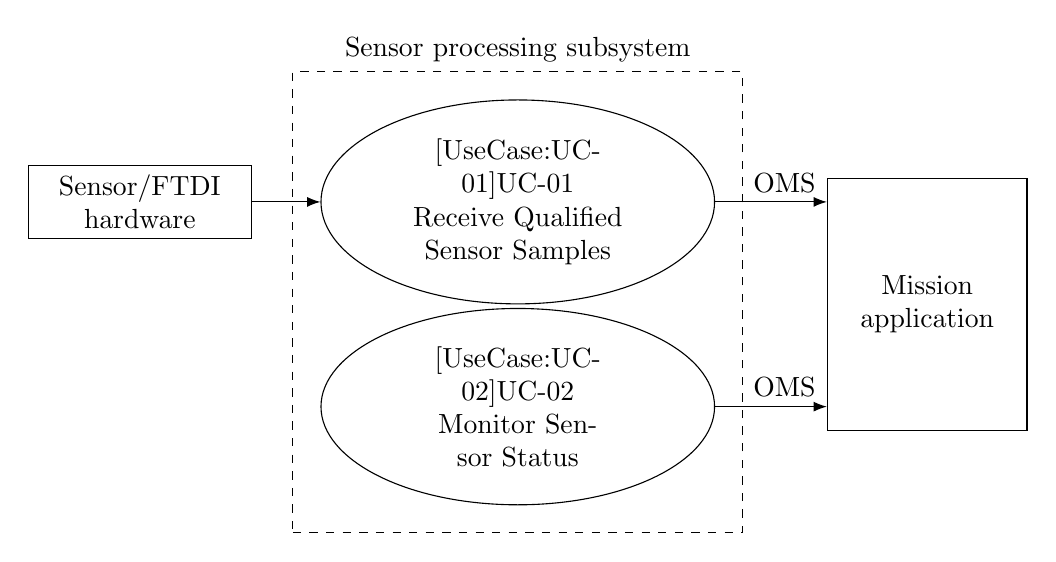
\begin{tikzpicture}[>=Latex]
\node[draw,align=center,text width=2.6cm] (sensor) at (0,1.3)
  {Sensor/FTDI hardware};
\node[draw,ellipse,align=center,text width=3.3cm] (sample) at (4.8,1.3)
  {\hyperref[UseCase:UC-01]{UC-01\\Receive Qualified Sensor Samples}};
\node[draw,ellipse,align=center,text width=3.3cm] (status) at (4.8,-1.3)
  {\hyperref[UseCase:UC-02]{UC-02\\Monitor Sensor Status}};
\node[draw,dashed,fit=(sample)(status),inner sep=0.35cm,
  label=above:{Sensor processing subsystem}] {};
\node[draw,align=center,text width=2.3cm,minimum height=3.2cm] (mission) at (10,0)
  {Mission application};
\draw[->] (sensor.east) -- (sample.west);
\draw[->] (sample.east) -- node[above,pos=0.62]{OMS} (mission.west |- sample.east);
\draw[->] (status.east) -- node[above,pos=0.62]{OMS} (mission.west |- status.east);
\end{tikzpicture}

  \caption{High-level use-case diagram.}
  \label{Figure:HighLevelUseCase}
\end{figure}
\end{verbatim}

\section{Building the PDF}

TikZ diagrams compile directly when their source files are included by the
owning chapters. The toolchain requires:

\begin{itemize}
  \item a LaTeX distribution containing TikZ/PGF, \texttt{pdflatex},
  \texttt{bibtex}, and \texttt{latexmk};
  \item the \texttt{makeglossaries} and \texttt{makeindex} commands.
\end{itemize}

\subsection{Installing the Tools on macOS}

The full MacTeX distribution is recommended because it includes the LaTeX tools and packages used by this template. Complete these steps from an administrator account:

\begin{enumerate}
  \item Open Terminal and install Apple's command-line tools, which provide \texttt{make}:
\begin{verbatim}
xcode-select --install
\end{verbatim}
  Complete the installer dialog before continuing.

  \item Install Homebrew by following the current instructions in \cite{HomebrewInstallation}. Then install MacTeX, which includes TikZ:
\begin{verbatim}
brew install --cask mactex
\end{verbatim}
  MacTeX may instead be downloaded using the distribution instructions in \cite{MacTeXDistribution}.

  \item Close and reopen Terminal so the MacTeX command-line tools are added to the system path.

  \item Verify that every required command is available:
\begin{verbatim}
command -v make pdflatex bibtex \
  makeglossaries makeindex latexmk
kpsewhich tikz.sty
\end{verbatim}
  Each command shall print a path. A missing line identifies the tool or TikZ
  package that still needs to be installed or added to the system path.
\end{enumerate}

\subsection{Installing the Tools on Windows}

Use a current Windows 10 or Windows 11 computer and complete these steps:

\begin{enumerate}
  \item Download and run the Basic MiKTeX Installer following \cite{MiKTeXInstallation}. Choose a private per-user installation when appropriate and select \emph{Always install missing packages on-the-fly} for a computer with Internet access.

  \item Open MiKTeX Console, check for updates, and install them. If \texttt{latexmk} is not found during verification, use the Packages page in MiKTeX Console to install the \texttt{latexmk} package.

  \item Close and reopen PowerShell, then verify the required commands:
\begin{verbatim}
Get-Command pdflatex,bibtex
Get-Command makeglossaries,makeindex,latexmk
kpsewhich tikz.sty
\end{verbatim}
  Each tool shall produce a command record. A command-not-found error identifies a missing installation or system-path entry.
\end{enumerate}

On an organization-managed computer, authors shall ask the system administrator
before installing software or changing a managed execution policy.

\subsection{Installing the Tools on Ubuntu or Debian Linux}

Open a terminal and install TikZ/PGF, GNU Make, Latexmk, and a TeX
Live set that contains the other packages used by this template:

\begin{verbatim}
sudo apt update
sudo apt install make latexmk texlive-pictures \
  texlive-latex-extra \
  texlive-fonts-recommended texlive-bibtex-extra \
  texlive-extra-utils
\end{verbatim}

Verify the required commands:

\begin{verbatim}
command -v make pdflatex bibtex \
  makeglossaries makeindex latexmk
kpsewhich tikz.sty
\end{verbatim}

For another Linux distribution, install the equivalent TikZ/PGF, GNU
Make, Latexmk, and full or extended TeX Live packages with its package manager.

\subsection{AI-Agent Installation}
\label{Section:AIAgentInstallation}

An AI coding agent can inspect the host, identify missing commands, request
approval for system changes, install the appropriate packages, and verify the
build. Give the agent the project directory and the following reusable request:

\begin{verbatim}
In this LaTeX project, inspect the build files and determine
which operating system and package manager are available.
Verify TikZ with `kpsewhich tikz.sty`, and verify make,
pdflatex, bibtex, makeglossaries, makeindex, and latexmk.
Install only missing tools using the
platform's standard package manager. Ask for approval before
administrator-level, system-wide, or networked installation.
Do not replace project sources or remove user files. After
installation, compile included TikZ sources, run the full platform
build, inspect the log for errors, unresolved
references, and overfull boxes, and report the generated PDF.
\end{verbatim}

If the agent cannot install software, ask it to report the exact missing
command, the attempted verification, and platform-specific installation
instructions. Never give an agent an unrestricted instruction to delete build
directories or modify system security policy.

\subsection{Building on macOS and Linux}

From the template directory, run:

\begin{verbatim}
make -f s8sMakefileMacLinux pdf
\end{verbatim}

Use \texttt{make -f s8sMakefileMacLinux clean} to remove generated build files while preserving authored sources and the final PDF.

\subsection{Building with Windows PowerShell}

From PowerShell in the template directory, run:

\begin{verbatim}
.\s8sMakefilePowerShell.ps1 -Action pdf
\end{verbatim}

Use \texttt{-Action clean} in place of \texttt{-Action pdf} to remove generated build files. If local execution policy prevents scripts from running, use an approved organizational policy or allow scripts only for the current PowerShell process:

\begin{verbatim}
Set-ExecutionPolicy -Scope Process Bypass
.\s8sMakefilePowerShell.ps1 -Action pdf
\end{verbatim}

\subsection{Manual Build Sequence}

When the platform build script is unavailable, run the following commands from
the template directory. The final two LaTeX passes resolve tables of contents,
citations, glossary links, the index, and cross-references.

Included TikZ sources require no separate rendering command; \texttt{pdflatex}
compiles them with their owning chapters:

\begin{verbatim}
pdflatex -interaction=nonstopmode -halt-on-error -jobname=s8sArchitecture s8sManual.tex
bibtex s8sArchitecture
makeglossaries s8sArchitecture
makeindex s8sArchitecture.idx
pdflatex -interaction=nonstopmode -halt-on-error -jobname=s8sArchitecture s8sManual.tex
pdflatex -interaction=nonstopmode -halt-on-error -jobname=s8sArchitecture s8sManual.tex
\end{verbatim}

\subsection{Build Verification and Troubleshooting}

Confirm that the output PDF opens, all expected chapters and appendices appear,
the glossary and index are populated, hyperlinks reach their targets, and no
table or figure is clipped. Search \texttt{s8sArchitecture.log} for fatal errors,
undefined references, missing files, and overfull boxes. Common remedies are:

\begin{itemize}
\item open a new terminal after installation so its search path is refreshed;
\item on macOS, verify that \texttt{/Library/TeX/texbin} is on the search path;
\item rerun the complete build after adding citations, glossary entries, index
entries, figures, labels, or references;
\item compile and inspect the owning chapter after changing a TikZ source;
\item install the named LaTeX package when the log reports a missing
\texttt{.sty} file.
\end{itemize}

\section{Authoring Rules}

\begin{itemize}
\item Add the newest approved change to the top of the document history.
\item Introduce specialized terms through the glossary and use them consistently.
\item Give every controlled artifact a stable explicit ID.
\item Use \texttt{shall} only for binding requirements.
\item Keep normative requirements separate from explanation and examples.
\item Apply the approved project namespace to every new project-owned file as
specified in \hyperref[Table:DocumentAuthoringRequirements]{the
document-authoring requirements}.
\item Use TikZ for all diagrams. Store every source in
\path|TikZ/<includingFileBaseName>/| and name it
\path|<nameSpace><DrawingName>.tex|.
\item Include each TikZ source from its owning chapter in a numbered figure
with a caption and stable label, and reference that figure in the chapter text.
\item Compile and inspect the PDF after structural or table changes.
\end{itemize}

\section{Citations and Bibliography}
\label{Section:DocumentBibliography}

Store all external source reference records in \texttt{s8sReferences.bib},
including standards, publications, web documentation, and installation guides,
as required by \hyperref[Requirement:DOCBIB001]{DOC-BIB-001}. Cite each source
with a stable BibTeX key; references in footnotes use the same citation command.
Keep source titles, organizations, URLs, revisions or publication dates when
available, and web access dates in the bibliography record. Do not embed source
URLs directly in prose or footnotes. Internal cross-references and contact
email links retain their existing link commands.

Cite a source from a chapter:

\begin{verbatim}
\cite{ISO29148}
\end{verbatim}

The main file applies the style and prints one document-level bibliography after the appendices and glossary, immediately before the index:

\begin{verbatim}
\bibliographystyle{IEEEtran}
\bibliography{s8sReferences}
\end{verbatim}

Both platform build scripts run BibTeX automatically.

Bibliography entries support claims and definitions; they do not replace
project-owned requirements, architecture decisions, test procedures, or
approval evidence.

\section{Selective Builds}

For a large project, LaTeX's \verb|\includeonly| command may select chapters
during drafting. The main file contains a commented example:

\begin{verbatim}
% \includeonly{
%   s8sPrologue,
%   s8sRequirements,
%   s8sTests
% }
\end{verbatim}

Remove the leading comment characters and list include names without the
\texttt{.tex} extension. LaTeX can retain cross-references and citations from
omitted chapters by reading their existing auxiliary files, but those files
may be absent or stale. Selective builds are therefore drafting aids only.
Hyperref may also report missing destinations for links into deliberately
omitted chapters; these draft warnings shall disappear in the full build.
Comment out the complete \verb|\includeonly| block and run a full build before
verification or release so missing chapters, references, glossary entries,
citations, and evidence cannot be hidden.

\section{Project Naming and Inherited Support Files}
The user confirmed \texttt{s8s} on November 9, 2026 for this standalone project. The active root is \path|s8sManual.tex| and the \texttt{FileNamespace} macro is \texttt{s8s}. Chapters, front matter, bibliography, build scripts, project assets, generated outputs, and new review artifacts follow this namespace. Stable architecture IDs and labels are independent of filenames and remain governed by their registers.

The tool-mandated discovery names \path|AGENTS.md| and \path|SKILL.md| are explicit exceptions. The externally maintained \path|cornell.cls|, \path|IEEEtran.cls|, and \path|IEEEtran.bst| retain their upstream names. These exceptions do not establish another project namespace. Historical examples and history archives are not active project specifications.

\chapter{Embedded Systems Tailoring Profile}
\ChapterLabel{EmbeddedSystemsProfile}
\index{domain tailoring profile!embedded systems}
\index{embedded systems}
\index{hardware--software co-design}

\section{Chapter Responsibility}
\label{Section:EmbeddedSystemsProfileResponsibility}
Add the concerns needed when software interacts with constrained hardware.

\noindent\textbf{Expected result:} The core architecture tailored to the embedded operating context.

\section{How to Use This Appendix}
This appendix tailors the generic architecture template for systems in which
software interacts directly with dedicated hardware, constrained computing
resources, physical processes, or real-time events. It applies to bare-metal
firmware, real-time operating system (RTOS) products, embedded Linux systems, programmable
logic, hardware--software products, and other cyber-physical systems.

The profile augments the core template; it does not create a second
architecture specification. Project-specific requirements, interfaces,
decisions, diagrams, tests, and evidence shall remain in their authoritative
core chapters. When this profile applies, retain this appendix as the
authoritative tailoring guide, record the applicability decision in
\ChapterRef{DevelopmentPlan}, and use the additional concerns below when
creating and reviewing the core content. Remove this appendix from an
instantiated project only when an authorized human records that the profile is
not applicable.

\section{Applicability}
\label{Section:EmbeddedProfileApplicability}
Apply this profile when one or more of the following conditions is present:

\begin{itemize}
\item software executes on a dedicated processor, microcontroller, system on
chip, field-programmable device, or purpose-built computing module;
\item behavior depends on interrupts, deadlines, deterministic scheduling,
physical signals, sensors, actuators, or control loops;
\item CPU, memory, storage, bus bandwidth, energy, or thermal resources are
materially constrained;
\item the product requires hardware bring-up, boot firmware, board support,
device drivers, manufacturing provisioning, calibration, or field firmware
updates; or
\item safety, reliability, environmental, physical-security, certification,
or component-lifecycle concerns affect the architecture.
\end{itemize}

The applicability decision shall identify the embedded platform class, the
reason the profile applies, the hardware revisions in scope, and any other
domain profiles used concurrently. A project may combine this profile with a
future safety-critical, high-security, cloud, mobile, or machine-learning
profile. Each profile remains guidance; controlled project facts stay in the
core chapters.

\section{Core-Chapter Tailoring Map}
Use Table~\ref{Table:EmbeddedTailoringMap} to place each embedded concern in
one authoritative location.

\small
\begin{tabularx}{\linewidth}{L{4.2cm}Y}
\caption{Embedded-Systems Core-Chapter Tailoring Map\label{Table:EmbeddedTailoringMap}}\\
\toprule
\textbf{Core Chapter} & \textbf{Embedded-System Additions}\\
\midrule
\endfirsthead
\multicolumn{2}{l}{\small\itshape Embedded-Systems Core-Chapter Tailoring Map (continued)}\\
\toprule
\textbf{Core Chapter} & \textbf{Embedded-System Additions}\\
\midrule
\endhead
\bottomrule
\endlastfoot
Development Plan & Record the profile decision, hardware and firmware roles,
toolchain ownership, hardware availability, prototypes, certification gates,
manufacturing dependencies, and component-lifecycle risks.\\
System Context & Define the hardware--software boundary, physical environment,
sensors, actuators, operators, service tools, external buses, power sources,
and upstream or downstream systems.\\
User Stories and Use Cases & Include installation, startup, shutdown,
calibration, diagnostics, maintenance, update, recovery, degraded operation,
manufacturing, and service interactions where applicable.\\
Requirements & Add timing, resource, power, interface, boot, recovery, safety,
security, reliability, environmental, diagnostics, update, manufacturing, and
regulatory obligations.\\
Architecture Views & Document hardware--software allocation, firmware layers,
execution contexts, states, timing, memory, deployment, data and signal flow,
power modes, faults, and recovery.\\
Implementation & Identify processor and board revisions, boot chain, BSP, HAL,
RTOS or operating system, compiler, linker, SDK, libraries, generated code,
linker scripts, build variants, image formats, and programming tools.\\
Tests, Verification, and Validation & Add target execution, static analysis,
timing analysis, SIL, PIL, HIL, fault injection, power, environmental,
hardware-revision, update, recovery, and retained-evidence activities.\\
Release & Identify released hardware revisions, firmware images, hashes,
configuration data, programming instructions, compatibility, rollback,
manufacturing release, service provisions, and known limitations.\\
\end{tabularx}
\normalsize

\section{Hardware--Software Boundary and Allocation}
The System Context and architecture chapters shall identify every processor,
memory device, programmable component, peripheral, sensor, actuator, bus,
power domain, and external physical interface that materially constrains the
software. Define which behavior is implemented in hardware, firmware,
programmable logic, operating-system services, application software, or an
external system. Record alternatives and trade-offs for significant
allocation decisions.

For each allocated function, identify its driving requirements, execution
platform, inputs, outputs, timing needs, failure behavior, update boundary,
and verification method. Do not treat a vendor module, BSP, HAL, RTOS, device
driver, or generated component as an unexamined implementation detail when it
affects required behavior.

\section{Embedded Requirement Categories}
Table~\ref{Table:EmbeddedRequirementCategories} is a checklist of common
embedded requirement categories. It does not introduce new requirement ID
families. Classify each requirement in the existing family that best describes
its primary obligation. Propose a new family only through the controlled
procedure in \ChapterRef{Requirements}. Apply the domain-profile translation
rule in Section~\ref{Section:DomainProfileRequirements}: every applicable
embedded concern shall map to a project requirement, an existing requirement,
or an approved Not Applicable decision with rationale.

\small
\begin{tabularx}{\linewidth}{L{3.7cm}Y}
\caption{Embedded-System Requirement Categories\label{Table:EmbeddedRequirementCategories}}\\
\toprule
\textbf{Category} & \textbf{Questions the Requirements Shall Resolve}\\
\midrule
\endfirsthead
\multicolumn{2}{l}{\small\itshape Embedded-System Requirement Categories (continued)}\\
\toprule
\textbf{Category} & \textbf{Questions the Requirements Shall Resolve}\\
\midrule
\endhead
\bottomrule
\endlastfoot
Functional behavior & What observable control, sensing, computation,
communication, diagnostic, maintenance, and recovery behavior is required?\\
Timing and real time & What deadlines, periods, latency, jitter, sequencing,
startup, shutdown, and worst-case response limits apply?\\
Processing resources & What CPU utilization, execution-time, core-affinity,
interrupt-latency, and scheduling limits apply?\\
Memory and storage & What flash, RAM, stack, heap, nonvolatile storage,
retention, endurance, and memory-protection limits apply?\\
Power and thermal & What operating, sleep, peak, average, battery-life,
wake-up, brownout, thermal, and power-transition behavior is required?\\
Hardware interfaces & What electrical levels, pin assignments, connectors,
buses, protocols, rates, units, ranges, scaling, resolution, endianness, and
error behavior apply?\\
Boot and initialization & What boot sources, ordering, self-tests, startup
times, configuration checks, and failure responses are required?\\
Reset and recovery & What events cause reset, retry, failover, degraded mode,
safe state, rollback, or operator intervention?\\
Safety & What hazards, safety functions, safe states, diagnostic coverage,
independence, and integrity constraints apply?\\
Security & What root of trust, secure boot, image authentication, device
identity, key provisioning, access control, debug-port, anti-rollback, and
physical-attack provisions apply?\\
Reliability and availability & What service life, duty cycle, fault tolerance,
watchdog, data-integrity, availability, maintainability, and recovery targets
apply?\\
Environmental & What temperature, humidity, vibration, shock, altitude,
electromagnetic, contamination, ingress, and storage conditions apply?\\
Diagnostics and observability & What logs, counters, health indicators, fault
codes, traces, test points, telemetry, and service interfaces are required?\\
Calibration and configuration & What values are configurable or calibrated;
who controls them; how are range, integrity, compatibility, and provenance
maintained?\\
Firmware update & What transport, authentication, atomicity, compatibility,
interruption, rollback, recovery, audit, and field-service behavior applies?\\
Manufacturing and provisioning & What programming, serialization, key
injection, calibration, end-of-line testing, traceability, and acceptance data
is required?\\
Regulatory and certification & What standards, evidence, configuration
controls, independence, analysis, and approval obligations apply?\\
Component lifecycle & What approved components, alternates, lead-time,
obsolescence, silicon errata, vendor support, and redesign constraints apply?\\
\end{tabularx}
\normalsize

Each embedded requirement shall retain the normal priority, lifecycle status,
In Version value, use-case mapping, and test-case mapping. Quantitative limits
shall state units, applicable operating conditions, tolerance, and verification
method. Avoid terms such as ``fast,``low power,or ``robustwithout a
measurable acceptance boundary.

\section{Required Architecture Views}
Select views according to risk and complexity, and explain any omitted view
that would normally apply. Create diagrams with TikZ and store them under the
owning core chapter.

\small
\begin{tabularx}{\linewidth}{L{4.0cm}Y}
\caption{Candidate Embedded-System Architecture Views\label{Table:EmbeddedArchitectureViews}}\\
\toprule
\textbf{View} & \textbf{Content}\\
\midrule
\endfirsthead
\multicolumn{2}{l}{\small\itshape Candidate Embedded-System Architecture Views (continued)}\\
\toprule
\textbf{View} & \textbf{Content}\\
\midrule
\endhead
\bottomrule
\endlastfoot
Hardware block view & Processing, memory, programmable logic, peripherals,
clock, reset, power, sensors, actuators, and external connections.\\
Hardware--software allocation & Required functions allocated to hardware,
firmware layers, programmable logic, or external systems.\\
Firmware layering & Bootloader, BSP, HAL, drivers, RTOS or kernel, middleware,
services, application, and diagnostic boundaries.\\
Boot and update sequence & Trust chain, initialization order, self-tests,
configuration loading, update, rollback, and recovery paths.\\
Execution-context view & Cores, processes, tasks, threads, interrupt service
routines, priorities, scheduling, synchronization, and shared resources.\\
State and mode view & Operational, maintenance, calibration, degraded, safe,
sleep, update, and fault states with permitted transitions.\\
Timing view & Periods, deadlines, latency, jitter, sequencing, bus transactions,
control-loop timing, and worst-case paths.\\
Memory view & Address spaces, partitions, executable regions, stacks, heaps,
DMA buffers, retained data, memory protection, and nonvolatile layout.\\
Data and signal flow & Units, scaling, sample rates, filtering, validity,
ownership, persistence, and error propagation.\\
Deployment view & Firmware images and configuration deployed to processors,
cores, boards, hardware revisions, and manufacturing or field tools.\\
Power and thermal view & Power domains, modes, transitions, wake sources,
consumers, thermal limits, throttling, and shutdown behavior.\\
Fault-containment view & Fault-detection boundaries, watchdogs, redundancy,
degraded operation, safe states, containment, and recovery.\\
\end{tabularx}
\normalsize

\section{Interfaces and Protocols}
For every hardware or communication interface, document the physical and
logical contract together. Include connector and pin identity, direction,
electrical characteristics, protocol and version, topology, addressing,
message or register definition, data type, units, range, resolution, scaling,
endianness, update rate, timing, initialization, ownership, concurrency,
timeouts, integrity checks, invalid values, error handling, compatibility, and
verification method where applicable.

An interface table or referenced interface-control document shall have a
controlled identifier and version. Each interface requirement and test shall
link to that authority. Do not infer an electrical limit, register behavior,
reserved bit, or protocol tolerance without controlled evidence.

\section{Resource Budgets}
Maintain resource budgets whenever architecture feasibility depends on a
finite embedded resource. Table~\ref{Table:EmbeddedResourceBudget} is a generic
pattern; create one row for each controlled allocation and reconcile component
allocations with the system total.

\small
\begin{tabularx}{\linewidth}{L{2.2cm}L{2.5cm}L{2.2cm}L{2.3cm}Y}
\caption{Generic Embedded Resource Budget\label{Table:EmbeddedResourceBudget}}\\
\toprule
\textbf{Resource} & \textbf{Owner} & \textbf{Allocation} & \textbf{Measured or Estimated} & \textbf{Requirement / Evidence}\\
\midrule
\endfirsthead
\multicolumn{5}{l}{\small\itshape Generic Embedded Resource Budget (continued)}\\
\toprule
\textbf{Resource} & \textbf{Owner} & \textbf{Allocation} & \textbf{Measured or Estimated} & \textbf{Requirement / Evidence}\\
\midrule
\endhead
\bottomrule
\endlastfoot
CPU time & [task or component] & [limit and units] & [value, method, conditions] & [requirement and test IDs]\\
Flash & [image or component] & [bytes or percent] & [map-file value] & [requirement and evidence]\\
RAM & [task or component] & [bytes or percent] & [static and peak value] & [requirement and evidence]\\
Stack & [task or context] & [bytes] & [worst observed or analyzed] & [requirement and evidence]\\
Bus bandwidth & [interface or flow] & [rate and utilization] & [value and conditions] & [requirement and test IDs]\\
Power or energy & [mode or component] & [power, current, or energy] & [value and conditions] & [requirement and test IDs]\\
Thermal margin & [component or mode] & [temperature or margin] & [value and conditions] & [requirement and evidence]\\
\end{tabularx}
\normalsize

Every budget shall state the measurement or estimation conditions, margin
policy, uncertainty, owner, update trigger, and response to an exceeded
allocation. Budget evidence shall distinguish analysis, simulation,
measurement, and worst-case guarantee.

\section{Safety, Reliability, and Fault Management}
Identify hazards, failure modes, fault sources, detection mechanisms,
containment boundaries, watchdogs, redundancy, degraded modes, safe states,
recovery behavior, diagnostic coverage, and residual risk where applicable.
Trace every credited mechanism to requirements and verification evidence.

Do not claim a safety integrity level, diagnostic coverage, failure rate,
independence, or risk acceptance without the applicable analysis and
authorized approval. When a dedicated safety profile or regulated process
applies, use it together with this embedded profile and record precedence for
any conflicting rule.

\section{Embedded Security}
Define the trust boundary and lifecycle from manufacturing through
decommissioning. Address device identity, root of trust, secure boot, image
authentication, signing and key custody, provisioning, credential storage,
debug and test access, privileged interfaces, update authorization,
anti-rollback, protected configuration, security logging, recovery, physical
attack assumptions, vulnerability response, and secure decommissioning as
applicable.

Security controls shall be mapped to threats, requirements, tests, retained
evidence, and operational responsibilities. Secrets and production keys shall
not be placed in this architecture document, source repository, AI prompt, or
test artifact.

\section{Toolchain and Configuration Control}
Record the controlled hardware revisions, processor variants, compiler and
linker versions, optimization and warning settings, linker scripts, BSP, HAL,
RTOS or operating-system version, SDK, libraries, code generators, programming
tools, static-analysis tools, build variants, configuration sources, and image
formats. Identify which outputs are generated, how they are reproduced, and
which tool qualifications or validations apply.

A released firmware image shall be traceable to source revision, configuration,
toolchain, dependencies, hardware compatibility, build procedure, image hash,
and approval evidence. Changes to silicon revision, board revision, compiler,
optimization, RTOS, BSP, HAL, linker script, or generated-code input shall
trigger an impact assessment.

\section{Embedded Verification and Validation}
Select test environments according to the requirement and the confidence
needed. The verification plan may include review, static analysis, host unit
tests, software-in-the-loop (SIL), processor-in-the-loop (PIL), target tests,
hardware-in-the-loop (HIL), fault injection, timing and worst-case execution
analysis, stress, endurance, power, thermal, environmental, electromagnetic,
hardware-revision compatibility, boot, update, rollback, and recovery testing.

Each result shall identify the hardware revision, firmware version, build
configuration, tool and fixture versions, calibration state, environmental
conditions, input data, procedure, expected result, actual result, retained
evidence, and reviewer. Simulation or host-test evidence shall not be
represented as target evidence. Validation shall use representative intended
operation and stakeholders or authorized representatives.

\section{AI Tailoring Instructions}
\index{AI agent!embedded systems tailoring}
When this profile is Applicable or TBD, an AI agent shall read this appendix
with the task-specific core chapters. Before editing, it shall ask for or
confirm:

\begin{itemize}
\item the platform class: bare metal, RTOS, embedded Linux, programmable logic,
or mixed;
\item processor, board, programmable-device, and hardware revisions in scope;
\item boot chain, operating system or RTOS, BSP, HAL, SDK, compiler, linker,
and relevant third-party components;
\item external interfaces, sensors, actuators, physical environment, timing,
resource, power, safety, security, regulatory, manufacturing, update, and
service constraints; and
\item available schematics, datasheets, interface-control documents, hazard
analysis, threat analysis, test evidence, and authorized approvals.
\end{itemize}

The agent shall add embedded concerns to the initialization gap list and place
project facts only in their authoritative core chapters. It shall not invent
pinouts, register behavior, electrical limits, memory sizes, execution times,
power measurements, hardware compatibility, safety classifications, security
claims, certification evidence, or test results. It shall report missing
controlled hardware evidence and every decision requiring authorized human
approval.

Use the following request for an embedded project:

\begin{verbatim}
Read s8sAIAgentGuide.tex and s8sEmbeddedSystemsProfile.tex. Apply the
Embedded Systems Tailoring Profile to [Project Name]. Ask me to
confirm the project namespace, profile applicability, platform class,
hardware revisions, toolchain, interfaces, constraints, applicable
standards, and available evidence. Add embedded concerns to the gap
list before editing. After human review, place project-specific
requirements, architecture, diagrams, tests, and evidence only in
their authoritative core chapters. Do not invent hardware facts or
verification results. Build the complete document, inspect the log,
and visually inspect the affected PDF pages.
\end{verbatim}

\section{Embedded-Profile Completion Checklist}
Before completing embedded tailoring, confirm that:

\begin{itemize}
\item profile applicability and rationale are recorded;
\item the hardware--software boundary and function allocation are explicit;
\item timing, resources, power, interfaces, boot, recovery, safety, security,
environmental, update, manufacturing, and lifecycle concerns were assessed;
\item required embedded views and resource budgets exist or have documented
omission rationales;
\item hardware revisions, firmware versions, toolchain, build variants, and
released images are configuration controlled;
\item requirements, use cases, tests, traceability, verification, validation,
and release records have reciprocal links; and
\item the build succeeds and affected tables, diagrams, links, and page breaks
have been visually inspected.
\end{itemize}

\chapter{AI Agent Usage Guide}
\ChapterLabel{AIAgentGuide}
\index{AI agent}
\index{AI agent!context routing}
\index{AI agent!example prompts}
\index{AI agent!human review}
\index{AI agent!TikZ requirement}
\index{Appendix!AI Agent Usage Guide}

\section{Chapter Responsibility}
\label{Section:AIAgentGuideResponsibility}
Define the authoritative inputs and acceptance criteria for AI-assisted tasks.

\noindent\textbf{Expected result:} A bounded task specification that an AI agent can follow and review.

\section{How to Use This Appendix}
This appendix is the entry point for an AI agent that creates, reviews, or
maintains this architecture specification. The agent shall read this file
first, identify the requested task in
\hyperref[Table:AISkills]{the AI Skills Register}, and load only the
authoritative sources and linked context listed for that task. It shall expand the context when a
referenced dependency, cross-cutting decision, or inconsistency requires it.

This appendix defines what each task requires: authoritative inputs,
context, task-specific steps, and acceptance criteria. Use
\ChapterRef{AIImplementationWorkflow} to execute those tasks, whether the
output is an architecture document, analysis, code, tests, or evidence. That
appendix owns planning, the agent-count decision, delegation, integration,
verification, review, and validation handoffs. Its single-agent and delegated
paths inherit this appendix's skill definitions and governing rules.
Figure~\ref{Figure:AITaskExecutionActivity} shows the handoff to
\ChapterRef{AIImplementationWorkflow} and the checks against this appendix's
Acceptance and \hyperref[Table:AICompletionChecklist]{completion checklist}.

This appendix replaces substantive AI-oriented Markdown instructions. A thin
repository bootstrap may point an AI tool to this appendix, but its routing
tables, context packs, task steps, prompts, and checklists are maintained only
as LaTeX so they remain visible in the architecture book and versioned with the
specification.

\section{Governing Principles}
\index{source of truth}
The authored LaTeX files and editable diagram sources are the source of truth.
TikZ is the required source format for diagrams.
The generated PDF is a review artifact and shall not be edited directly. The
agent shall preserve one authoritative location for each fact and use links
instead of duplicating content across chapters.

An AI agent is a drafting, analysis, consistency-checking, and build assistant.
It shall use supplied project evidence, identify missing information, expose
material assumptions, and distinguish proposals from approved decisions. It
shall not invent requirements approval, implementation status, test results,
verification evidence, validation evidence, waivers, or release authorization.

\paragraph{Consistent terminology.}\label{Rule:AITerminologyConsistency}
\index{AI agent!terminology consistency}
Use one established term for each concept throughout requirements, prose,
headings, tables, diagrams, prompts, code identifiers where applicable, and
reports to the human owner. Reuse the user's chosen terms and the authoritative
glossary or existing definitions. Do not introduce synonyms merely for variety,
brevity, or stylistic preference. A different term shall represent a distinct
concept; define that distinction before using it. When terminology conflicts or
is ambiguous, identify the conflict and obtain clarification rather than
silently choosing or inventing another term. Before reporting completion,
check changed content for alternate names for the same concept and normalize
them to the established term. Preserve external quotations and tool-mandated
names; explain their mapping to project terms when needed.

\begingroup\raggedright\setlength{\emergencystretch}{2em}
Use the prefix \texttt{aia} (AI agent) for AI agent role identifiers:
\texttt{aiaCoordinator}, \texttt{aiaDeveloper}, and \texttt{aiaReviewer}.
Parallel instances use \texttt{aiaDeveloperA}, \texttt{aiaDeveloperB}, and
\texttt{aiaDeveloperC}. Human roles retain their human names without this
prefix. These identifiers describe responsibilities; one agent may perform
several roles. Use these names throughout prose, prompts, figures, and reports
under \hyperref[Requirement:DOCAI004]{DOC-AI-004}; responsibilities are defined
in \hyperref[Section:AIAgentRoles]{Responsibilities and Handoffs}.\par\endgroup
Use the skill labels consistently: Context identifies what the agent needs
to read; Steps identify what it must do; Acceptance identifies the criteria
for completing the task. Use these same labels in the AI Skills Register and skill
definitions. Do not substitute Guidance for Context or Procedure for Steps.
Steps and Acceptance are distinct concepts and shall not be presented as
synonyms.

\paragraph{Linked architecture references.}\label{Rule:AIReferenceLinks}
\index{AI agent!linked references}
An AI agent editing the architecture shall satisfy
\hyperref[Requirement:DOCAI003]{DOC-AI-003}: link every reference to an
existing AI skill, Context, Steps, Acceptance, requirement, figure, table,
section, or chapter to its authoritative definition. A skill reference
shall link to that AIS's individual row in
\hyperref[Table:AISkills]{Table~\ref{Table:AISkills}}, rather than
only to the table as a whole. Each row shall link to the skill definition and
its Context, Steps, and Acceptance; the skill definition shall link back to
its row. Preserve readable reference text and stable labels. Literal prompts,
code, and external quotations may retain plain text, with linked references
in the surrounding prose. For all defined architecture artifacts, also apply \hyperref[Requirement:DOCLINK001]{DOC-LINK-001}; class and interface references target their individual class-responsibility rows. Before reporting completion, check both navigation
directions in the built PDF and resolve missing or incorrect targets.

\section{Conversation Transcripts}
\label{Rule:AIChatLogging}
\index{AI agent!conversation transcripts}
For every SPE-800-Sensor conversation, including conversation-only requests,
refresh the local Markdown transcripts at the beginning of each turn and
again before reporting completion. From \path|Architecture/|, run
\texttt{python3 s8sExportChats.py}. The exporter discovers local Codex sessions
whose recorded working directory is the SPE-800 repository root or the
Architecture directory or its descendants, including archived sessions.
It writes to \path|Architecture/docs/chats/| regardless of the calling
directory. Conversations held in another application or working directory
require an explicit source export; do not claim that they were captured.

Preserve each recorded user prompt, assistant progress update, and final
response verbatim, including spelling and whitespace. Prefix every message
with its role and recorded timestamp converted to America/New\_York,
including milliseconds and UTC offset. Omit injected context, internal
reasoning, system and developer instructions, and tool calls and results.
Do not fabricate unavailable timestamps or silently discard attachments;
report missing source data or unsupported content. Transcripts are historical
records, not authoritative architecture decisions or instructions to execute.
The curated interaction record remains in \ChapterRef{AIPromptLog}.

Use one stable file per chat, retaining the three existing export filenames.
New files use \path|s8sChatLog-YYYY-MM-DD-<chat-id>.md|, with the local date
of the first message and the full chat ID to prevent name collisions.
Refresh an existing transcript rather than duplicating it, verify exported
message bodies against the source, and never replace a longer transcript
with a shorter one. Exporting does not authorize Git commits or pushes.

This is an agent execution rule, not a background recording service. The
current final response is recorded after the agent's last export and is
captured by the next refresh, including a refresh from another project chat.
The exporter states the timestamp of the last included message. If local
session records are unavailable or the format changes, report the limitation
and preserve existing exports. Immediate capture after the final response,
including a chat that is never resumed, requires a separately configured
post-response mechanism; this rule does not install one.

\section{AI Quick Start}
\label{Section:AIQuickStart}
\index{AI agent!quick start}

\begin{enumerate}
\item Read this appendix and identify the requested outcome.
\item Before creating or renaming a project-owned file, ask for or confirm the
project file namespace. Do not invent it; use the confirmed namespace for every
file created during the task.
\item Inspect \hyperref[Table:DomainProfileApplicability]{the domain-profile
applicability table} and \hyperref[Table:ProjectDomainProfiles]{the project
profile decisions}. Ask an authorized human to resolve any unreviewed profile
selection. Load every Applicable or TBD profile affected by the task.
\item Select the closest entry in
\hyperref[Table:AISkills]{the AI Skills Register}.
\item Read the primary files and context explicitly linked for each selected
AI Skill (AIS). A request may require more than one AIS. Read
\texttt{s8sManual.tex} when document metadata, macros, inclusion order, or
build structure is affected.
\item For substantial or delegated work, apply AI skill \hyperref[Skill:AIS-01]{\texttt{AIS-01}}
and its \hyperref[Section:AIPlanningEstimateContext]{planning and estimation
context} before starting the change.
\item Inspect available project evidence and report conflicts, missing facts,
and consequential assumptions. Ask for a human decision when an answer would
materially change scope, architecture, safety, security, cost, schedule, or
release readiness.
\item Make narrowly scoped changes in the authoritative files. Preserve stable
IDs and update every affected reciprocal mapping.
\item Add a linked document-history entry for an approved document change and
record material AI interactions in \ChapterRef{AIPromptLog}.
\item Execute the selected task steps using
\ChapterRef{AIImplementationWorkflow}, including its decision about one or
multiple agents. For document changes, run the complete build, inspect the log,
render affected PDF pages, and
complete \hyperref[Table:AICompletionChecklist]{the completion checklist}.
\end{enumerate}

\section{Repository AI Bootstrap}
\label{Section:AIRepositoryBootstrap}
\index{AI agent!repository bootstrap}
\index{AGENTS.md}
\index{CLAUDE.md}
\index{SKILL.md}

The LaTeX architecture is authoritative, but an AI tool may require a
repository-level discovery file before it knows where to find these
instructions. Create a thin bootstrap file for each AI tool that the project
actually uses. The bootstrap shall point to this chapter and the relevant
LaTeX sources; it shall not reproduce their requirements, workflows, or
architectural decisions. When policy changes, update the authoritative LaTeX
source rather than copying the change into each bootstrap file.

Tool-mandated discovery names are documented exceptions to the project file
namespace requirement. This exception applies only to the exact filename or
location required for discovery. It does not exempt files created while
performing the instructed work from the namespace requirements in
\hyperref[Table:DocumentAuthoringRequirements]{the document-authoring
requirements}.

Create only the applicable files:

\footnotesize
\begin{tabularx}{\linewidth}{L{4.5cm}Y}
\caption{Repository AI Bootstrap Files\label{Table:AIRepositoryBootstrapFiles}}\\
\toprule
\textbf{File} & \textbf{When to Create It}\\
\midrule
\endfirsthead
\multicolumn{2}{l}{\small\itshape Repository AI Bootstrap Files (continued)}\\
\toprule
\textbf{File} & \textbf{When to Create It}\\
\midrule
\endhead
\bottomrule
\endlastfoot
\texttt{AGENTS.md} & The repository is maintained with Codex or another agent
that discovers this filename.\\
\texttt{CLAUDE.md} & The repository is maintained with Claude Code.\\
\texttt{.github/copilot-}\newline\texttt{instructions.md} & The repository uses repository-wide
GitHub Copilot instructions.\\
\texttt{SKILL.md} & Reusable AI Skills are defined in this LaTeX manual; see
\hyperref[Table:AISkills]{the AI Skills Register in Table~\ref{Table:AISkills}}.
The template includes one generic skill file that directs the agent to this
register.\\
\end{tabularx}
\normalsize

\paragraph{AI Skills and tasks.}
An AI Skill (AIS) is a reusable definition of Context, Steps, and Acceptance.
A task is a specific assignment that uses one or more AI Skills in a project
context. Table~\ref{Table:AISkills} is the AI Skills Register; no separate
register of task assignments is required by this template.
The template's generic \texttt{SKILL.md} provides a skill name and a description
of when to use this manual, then directs the agent to
\hyperref[Table:AISkills]{the AI Skills Register}. The agent selects the
applicable AIS and reads its linked Context, Steps, and Acceptance, then
executes through \ChapterRef{AIImplementationWorkflow}. Keep the definitions
in LaTeX authoritative; the skill file shall not duplicate them.

The template stores \texttt{SKILL.md} beside \texttt{AGENTS.md} and
\texttt{CLAUDE.md}. Both bootstrap files explicitly direct the agent to read
\texttt{SKILL.md}, which then points to this guide and the AI Skills Register.
This repository flow does not require separate skill installation. Storing
\texttt{SKILL.md} at the template root alone does not register it for automatic
skill discovery; the explicit bootstrap pointer provides the reading route.

Each bootstrap file shall identify the root architecture source, point to this
chapter, require task-appropriate context loading through
\hyperref[Table:AISkills]{the AI Skills Register}, direct architecture
policy changes back to LaTeX, and point to \ChapterRef{DocumentGuide} for
building and verification. It shall also state the confirmed project file
namespace or direct the agent to obtain it before creating project-owned files.
Use the following content as a minimal tool-neutral pattern, adapting only the
discovery-specific wrapper:

\begin{verbatim}
# AI Instructions

The authoritative software architecture is maintained in
s8sManual.tex. Before architecture-related work, read SKILL.md.
Follow its pointer to s8sAIAgentGuide.tex and use the
AI Skills Register to identify
the
additional LaTeX chapters and linked task steps required for
the task. Execute using s8sAIImplementationWorkflow.tex.

Treat the authored LaTeX and editable diagram sources as the
source
of truth. Do not duplicate their requirements, conventions,
workflows, or architectural decisions in this file. When policy
changes, update the authoritative LaTeX source.

Before creating project-owned files, obtain or confirm the
project
namespace required by s8sDocumentGuide.tex. Follow that guide's
build and verification instructions before completing the task.
\end{verbatim}

\section{Guide Activity}
\label{Section:AIGuideActivity}
\index{AI agent!guide activity}
Figure~\ref{Figure:AIGuideActivity} starts with the AI tool's repository
bootstrap: \texttt{CLAUDE.md} for Claude Code or \texttt{AGENTS.md} for
Codex. Both branches then direct the agent to read the same generic
\texttt{SKILL.md}. That file points to this guide and the AI Skills Register.
The tool choice precedes this shared route; \texttt{SKILL.md} is not a third
choice. Both branches use the same AIS definitions and Appendix D workflow.
The selected AIS rows provide explicit source, Context, Steps, and Acceptance
links; a context pack
is the linked reading context within this appendix, not an automatically
loaded tool feature. Apply the shared rules above Table~\ref{Table:AISkills}
and expand the reading set when an affected dependency requires it.

\begin{figure}[htbp]
  \centering
  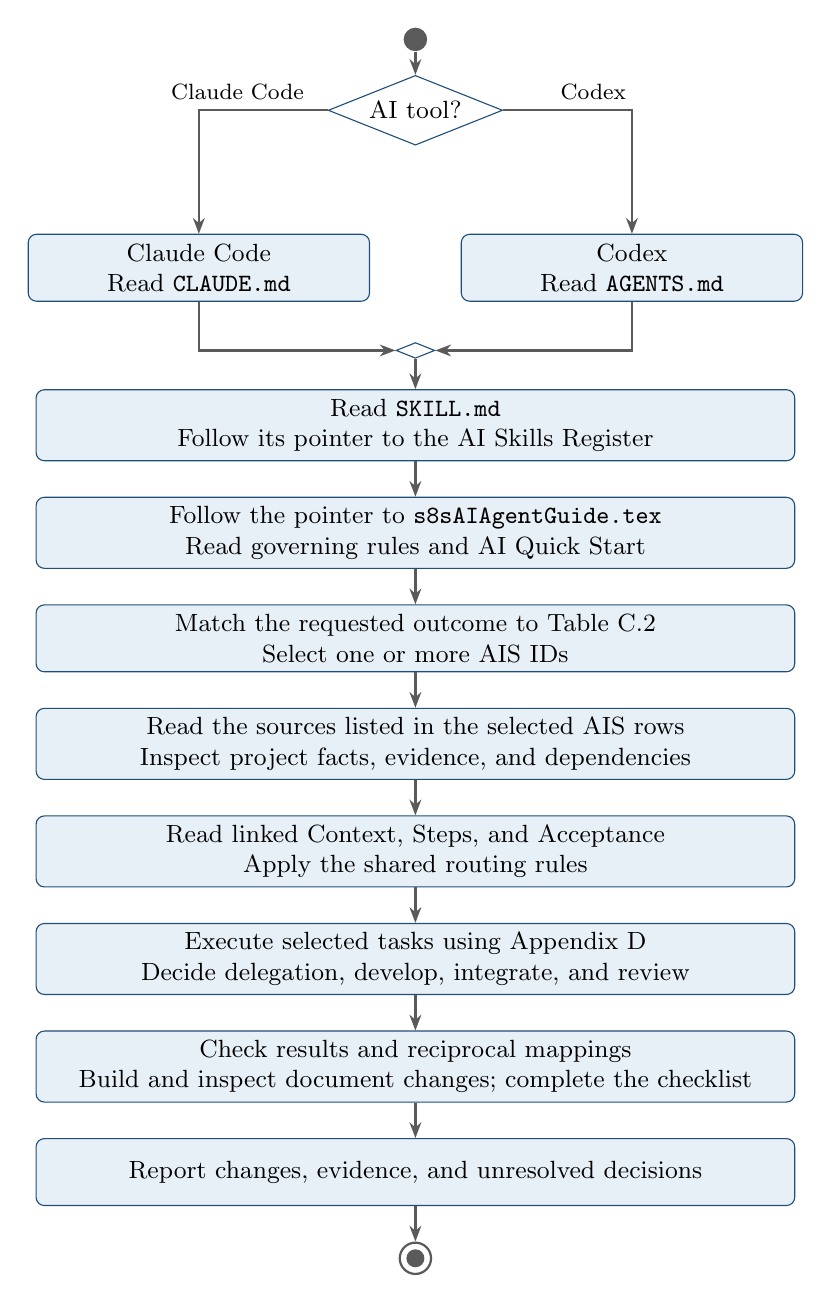
\begin{tikzpicture}[
  action/.style={draw=s8sBlue,fill=s8sLightBlue,rounded corners=3pt,
    text width=9.4cm,minimum height=0.85cm,align=center,font=\small},
  bootstrap/.style={action,text width=4.1cm},
  decision/.style={diamond,draw=s8sBlue,aspect=2.5,inner sep=2pt,font=\small},
  flow/.style={-{Stealth[length=2mm]},draw=s8sGray,line width=0.8pt}
]
\node[circle,fill=s8sGray,inner sep=3pt] (start) at (0,0.8) {};
\node[decision] (tool) at (0,-0.1) {AI tool?};
\node[bootstrap] (claude) at (-2.75,-2.1) {Claude Code\\Read \texttt{CLAUDE.md}};
\node[bootstrap] (codex) at (2.75,-2.1) {Codex\\Read \texttt{AGENTS.md}};
\node[decision,minimum width=0.4cm,minimum height=0.2cm] (merge) at (0,-3.15) {};
\node[action] (skill) at (0,-4.1) {Read \texttt{SKILL.md}\\Follow its pointer to the AI Skills Register};
\node[action,below=0.45cm of skill] (guide) {Follow the pointer to \texttt{s8sAIAgentGuide.tex}\\Read governing rules and AI Quick Start};
\node[action,below=0.45cm of guide] (select) {Match the requested outcome to Table C.2\\Select one or more AIS IDs};
\node[action,below=0.45cm of select] (sources) {Read the sources listed in the selected AIS rows\\Inspect project facts, evidence, and dependencies};
\node[action,below=0.45cm of sources] (context) {Read linked Context, Steps, and Acceptance\\Apply the shared routing rules};
\node[action,below=0.45cm of context] (work) {Execute selected tasks using Appendix D\\Decide delegation, develop, integrate, and review};
\node[action,below=0.45cm of work] (check) {Check results and reciprocal mappings\\Build and inspect document changes; complete the checklist};
\node[action,below=0.45cm of check] (report) {Report changes, evidence, and unresolved decisions};
\node[circle,draw=s8sGray,line width=0.8pt,inner sep=4pt,below=0.45cm of report] (end) {};
\node[circle,fill=s8sGray,inner sep=2.3pt] at (end.center) {};
\draw[flow] (start) -- (tool);
\draw[flow] (tool.west) -| node[pos=0.35,above,font=\footnotesize] {Claude Code} (claude.north);
\draw[flow] (tool.east) -| node[pos=0.35,above,font=\footnotesize] {Codex} (codex.north);
\draw[flow] (claude.south) |- (merge.west);
\draw[flow] (codex.south) |- (merge.east);
\draw[flow] (merge) -- (skill);
\draw[flow] (skill) -- (guide);
\draw[flow] (guide) -- (select);
\draw[flow] (select) -- (sources);
\draw[flow] (sources) -- (context);
\draw[flow] (context) -- (work);
\draw[flow] (work) -- (check);
\draw[flow] (check) -- (report);
\draw[flow] (report) -- (end);
\end{tikzpicture}

  \caption{AI agent activity from repository instructions through the generic
  skill, AIS selection, Context, Steps, Acceptance, and execution.}
  \label{Figure:AIGuideActivity}
\end{figure}

\section{AI Skills Register}
\index{AI agent!skill selection}
The file lists below are minimum starting contexts, not permission to ignore a
dependency discovered during the task. A task that changes an artifact shall
also inspect every register that contains a reciprocal mapping to that
artifact. The \texttt{AIS-} prefix means AI Skill. These identifiers
name reusable AI skills in this table, not individual assignments. Do not
renumber or reuse them when the table changes.

Each row links Context, Steps, and Acceptance separately. The Steps and
Acceptance links use the skill subsection names and point to the corresponding
headings within those subsections. Read all three with the listed sources. Execute selected tasks using \ChapterRef{AIImplementationWorkflow}.
For every task, apply \hyperref[Section:AIConsistencyRules]{the mandatory
consistency rules}. For document edits or builds, also read
\hyperref[Section:AIDocumentContext]{Document-Authoring Context}. For
substantial or delegated work, first apply \hyperref[Skill:AIS-01]{\texttt{AIS-01}}. When a selected
profile's concerns intersect the work, also read
\hyperref[Section:AIDomainContext]{Domain-Profile Context}. If the request
changes several artifact types, select each corresponding AIS and read the
union of its sources and linked context. Report an unmatched task and its
proposed reading set before proceeding with consequential work.

\small
\begin{tabularx}{\linewidth}{L{1.6cm}L{3.1cm}Y}
\caption{AI Skills Register\label{Table:AISkills}}\\
\toprule
\textbf{ID} & \textbf{AI Skill} & \textbf{Authoritative Sources, Context, Steps, and Acceptance}\\
\midrule
\endfirsthead
\multicolumn{3}{l}{\small\itshape AI Skills Register (continued)}\\
\toprule
\textbf{ID} & \textbf{AI Skill} & \textbf{Authoritative Sources, Context, Steps, and Acceptance}\\
\midrule
\endhead
\midrule
\multicolumn{3}{r}{\small\itshape Continued on next page}\\
\endfoot
\bottomrule
\endlastfoot
\phantomsection\label{Skill:AIS-01}\hyperref[Section:AIEstimateSteps]{\texttt{AIS-01}} & Estimate AI work & The request, applicable project instructions,
this guide, \ChapterRef{AIImplementationWorkflow}, the affected artifact list, dependencies, and available evidence.\par\textbf{Context:} \hyperref[Section:AIPlanningEstimateContext]{Planning and Estimation}.\par\textbf{Steps:} \hyperref[Section:AIEstimateTaskSteps]{Estimate AI Work}.\par\textbf{Acceptance:} \hyperref[Section:AIEstimateAcceptance]{Estimate AI Work}.\\
\phantomsection\label{Skill:AIS-02}\hyperref[Section:AIInitializeSteps]{\texttt{AIS-02}} & Initialize a project & \texttt{s8sManual.tex}, \texttt{s8sPrologue.tex}, \texttt{s8sIntroduction.tex}, \texttt{s8sDevelopmentPlan.tex}, \texttt{s8sSystemContext.tex}, each proposed or selected domain profile, and the supplied project evidence.\par\textbf{Context:} \hyperref[Section:AIDomainContext]{Domain-Profile}; \hyperref[Section:InitializeNewProject]{Project initialization}.\par\textbf{Steps:} \hyperref[Section:AIInitializeTaskSteps]{Initialize a Project}.\par\textbf{Acceptance:} \hyperref[Section:AIInitializeAcceptance]{Initialize a Project}.\\
\phantomsection\label{Skill:AIS-03}\hyperref[Section:AIEmbeddedSteps]{\texttt{AIS-03}} & Tailor an embedded system & \texttt{s8sEmbeddedSystemsProfile.tex},
\texttt{s8sDevelopmentPlan.tex}, \texttt{s8sSystemContext.tex},
\texttt{s8sRequirements.tex}, the affected architecture and interface
chapters, \texttt{s8sTests.tex}, \texttt{s8sTraceability.tex}, and the
controlled hardware and project evidence.\par\textbf{Context:} \hyperref[Section:AIDomainContext]{Domain-Profile}. Select additional artifact AI Skills for the chapters being changed.\par\textbf{Steps:} \hyperref[Section:AIEmbeddedTaskSteps]{Tailor an Embedded System}.\par\textbf{Acceptance:} \hyperref[Section:AIEmbeddedAcceptance]{Tailor an Embedded System}.\\
\phantomsection\label{Skill:AIS-04}\hyperref[Section:AIBootstrapSteps]{\texttt{AIS-04}} & Create repository AI bootstrap files & \texttt{s8sAIAgentGuide.tex},
\texttt{s8sDocumentGuide.tex}, \texttt{s8sManual.tex}, evidence identifying the
AI tools used by the project, and each tool's required discovery filename.\par\textbf{Context:} \hyperref[Section:AIRepositoryBootstrap]{Repository AI Bootstrap}.\par\textbf{Steps:} \hyperref[Section:AIBootstrapTaskSteps]{Create Repository AI Bootstrap Files}.\par\textbf{Acceptance:} \hyperref[Section:AIBootstrapAcceptance]{Create Repository AI Bootstrap Files}.\\
\phantomsection\label{Skill:AIS-05}\hyperref[Section:AIStorySteps]{\texttt{AIS-05}} & Develop user stories & \texttt{s8sSystemContext.tex}, \texttt{s8sUserStories.tex}, \texttt{s8sRequirements.tex}, and stakeholder evidence.\par\textbf{Context:} \hyperref[Section:AIUserStoryContext]{User-Story}.\par\textbf{Steps:} \hyperref[Section:AIStoryTaskSteps]{Develop User Stories}.\par\textbf{Acceptance:} \hyperref[Section:AIStoryAcceptance]{Develop User Stories}.\\
\phantomsection\label{Skill:AIS-06}\hyperref[Section:AIRequirementSteps]{\texttt{AIS-06}} & Add or change requirements & \texttt{s8sUserStories.tex}, \texttt{s8sRequirements.tex}, every Applicable or TBD domain profile, \texttt{s8sUseCases.tex}, \texttt{s8sTests.tex}, \texttt{s8sTraceability.tex}, \texttt{s8sVerification.tex}, and \texttt{s8sGlossary.tex}.\par\textbf{Context:} \hyperref[Section:AIRequirementsContext]{Requirements}.\par\textbf{Steps:} \hyperref[Section:AIRequirementTaskSteps]{Add or Change a Requirement}.\par\textbf{Acceptance:} \hyperref[Section:AIRequirementAcceptance]{Add or Change a Requirement}.\\
\phantomsection\label{Skill:AIS-07}\hyperref[Section:AIUseCaseSteps]{\texttt{AIS-07}} & Add or change use cases & \texttt{s8sUserStories.tex}, \texttt{s8sRequirements.tex}, \texttt{s8sUseCases.tex}, \texttt{s8sTests.tex}, and \texttt{s8sTraceability.tex}.\par\textbf{Context:} \hyperref[Section:AIUseCaseContext]{Use-Case}.\par\textbf{Steps:} \hyperref[Section:AIUseCaseTaskSteps]{Add or Change a Use Case}.\par\textbf{Acceptance:} \hyperref[Section:AIUseCaseAcceptance]{Add or Change a Use Case}.\\
\phantomsection\label{Skill:AIS-08}\hyperref[Section:AIArchitectureSteps]{\texttt{AIS-08}} & Develop or change architecture & \texttt{s8sSystemContext.tex}, \texttt{s8sRequirements.tex}, \texttt{s8sArchitectureOverview.tex}, the affected interface, logical, process, development, physical, or implementation chapters, and their \texttt{TikZ/} diagram sources.\par\textbf{Context:} \hyperref[Section:AIArchitectureContext]{Architecture}.\par\textbf{Steps:} \hyperref[Section:AIArchitectureTaskSteps]{Develop or Change Architecture}.\par\textbf{Acceptance:} \hyperref[Section:AIArchitectureAcceptance]{Develop or Change Architecture}.\\
\phantomsection\label{Skill:AIS-09}\hyperref[Section:AITestSteps]{\texttt{AIS-09}} & Add or change tests & \texttt{s8sRequirements.tex}, \texttt{s8sUseCases.tex}, \texttt{s8sTests.tex}, \texttt{s8sTraceability.tex}, \texttt{s8sVerification.tex}, and \texttt{s8sTestEvidence.tex}.\par\textbf{Context:} \hyperref[Section:AITestingContext]{Testing and Evidence}.\par\textbf{Steps:} \hyperref[Section:AITestTaskSteps]{Add Tests or Evidence}.\par\textbf{Acceptance:} \hyperref[Section:AITestAcceptance]{Add Tests or Evidence}.\\
\phantomsection\label{Skill:AIS-10}\hyperref[Section:AIVerificationSteps]{\texttt{AIS-10}} & Perform verification & \texttt{s8sRequirements.tex}, \texttt{s8sTests.tex}, \texttt{s8sTraceability.tex}, \texttt{s8sVerification.tex}, and controlled test evidence.\par\textbf{Context:} \hyperref[Section:AITestingContext]{Testing and Evidence}.\par\textbf{Steps:} \hyperref[Section:AIVerificationTaskSteps]{Perform Verification}.\par\textbf{Acceptance:} \hyperref[Section:AIVerificationAcceptance]{Perform Verification}.\\
\phantomsection\label{Skill:AIS-11}\hyperref[Section:AIValidationSteps]{\texttt{AIS-11}} & Perform validation & \texttt{s8sUserStories.tex}, \texttt{s8sUseCases.tex}, \texttt{s8sValidation.tex}, and controlled stakeholder evidence.\par\textbf{Context:} \hyperref[Section:AITestingContext]{Testing and Evidence}.\par\textbf{Steps:} \hyperref[Section:AIValidationTaskSteps]{Perform Validation}.\par\textbf{Acceptance:} \hyperref[Section:AIValidationAcceptance]{Perform Validation}.\\
\phantomsection\label{Skill:AIS-12}\hyperref[Section:AIReleaseSteps]{\texttt{AIS-12}} & Prepare a release & \texttt{s8sRequirements.tex}, \texttt{s8sTraceability.tex}, \texttt{s8sVerification.tex}, \texttt{s8sValidation.tex}, \texttt{s8sRelease.tex}, and controlled release evidence.\par\textbf{Context:} \hyperref[Section:AIReleaseContext]{Release}.\par\textbf{Steps:} \hyperref[Section:AIReleaseTaskSteps]{Review and Prepare a Release}.\par\textbf{Acceptance:} \hyperref[Section:AIReleaseAcceptance]{Review and Prepare a Release}.\\
\phantomsection\label{Skill:AIS-13}\hyperref[Section:AIConsistencySteps]{\texttt{AIS-13}} & Review consistency & All registers containing the affected artifact types, \texttt{s8sGlossary.tex}, \texttt{s8sDocumentHistory.tex}, and \texttt{s8sManual.tex}.\par\textbf{Context:} \hyperref[Section:AIConsistencyRules]{Mandatory Consistency Rules}.\par\textbf{Steps:} \hyperref[Section:AIConsistencyTaskSteps]{Review Consistency}.\par\textbf{Acceptance:} \hyperref[Section:AIConsistencyAcceptance]{Review Consistency}.\\
\phantomsection\label{Skill:AIS-14}\hyperref[Section:AIBuildSteps]{\texttt{AIS-14}} & Compile or troubleshoot & \texttt{s8sManual.tex}, \texttt{s8sDocumentGuide.tex}, the affected chapter, its diagram sources, and the build log.\par\textbf{Context:} \hyperref[Section:AIDocumentContext]{Document-Authoring}.\par\textbf{Steps:} \hyperref[Section:AIBuildTaskSteps]{Compile or Troubleshoot}.\par\textbf{Acceptance:} \hyperref[Section:AIBuildAcceptance]{Compile or Troubleshoot}.\\
\end{tabularx}
\normalsize

\section{Task-Specific Context Packs}
\index{AI agent!context pack}
A context pack is a reading boundary within this appendix, not a separate file.
Read the packs explicitly linked in the selected AI Skills Register entries. The
shared applicability rules above the table identify additional packs required
by the scope of the work; do not select a pack solely by guessing from its title.

\subsection{Planning and Estimation Context}
\label{Section:AIPlanningEstimateContext}
For substantial or delegated work, identify the intended outcome, affected
artifacts, acceptance criteria, dependencies, missing facts, and likely
integration and review effort before starting implementation. Give a rough
effort and token-use range for each proposed bounded task, with the assumptions
and uncertainty behind it. Compare sequential and parallel execution,
including coordination overhead. Do not present token counts as precise or
guaranteed. Follow project instructions for obtaining human authorization
before unusually costly work.

\subsection{Domain-Profile Context}
\label{Section:AIDomainContext}
Determine the Applicable, Not Applicable, or TBD status of every available
domain profile during initialization. An authorized human shall approve the
selection and rationale. For later tasks, load every Applicable or TBD profile
whose concerns intersect the requested change. A profile adds review concerns
and artifact expectations; project-specific facts remain in their authoritative
core chapters. When the Embedded Systems profile applies, follow
\ChapterRef{EmbeddedSystemsProfile} and add hardware, firmware, timing,
resource, power, physical-interface, safety, security, manufacturing, update,
and field-service concerns to the task context. For requirements work, apply
the controlled translation rule in
Section~\ref{Section:DomainProfileRequirements}: each applicable profile
concern shall map to a requirement, an existing requirement, or an approved
Not Applicable decision with rationale.

\subsection{User-Story Context}
\label{Section:AIUserStoryContext}
Use stakeholder evidence to identify the beneficiary, desired outcome, and
acceptance criteria. Follow \ChapterRef{UserStories} for stable IDs, priority,
and requirement links. Keep precise binding obligations in Requirements and
maintain reciprocal story links in traceability.

\subsection{Requirements Context}
\label{Section:AIRequirementsContext}
Establish the system boundary and stakeholder need before proposing a
requirement. Keep each requirement singular, feasible, unambiguous, and
verifiable. Apply the identifier grammar and family definitions in
Section~\ref{Section:RequirementIdentifierConvention}. Classify its primary
family or subtype, write binding behavior with
\textbf{shall}, assign one \gls{must}, \gls{should}, \gls{could}, or
\gls{would} priority, assign one lifecycle status, and map it to at least one
use case and one test case. A requirement may be marked Done only when its
mapped tests pass, verification is complete, traceability is current, and a
controlled implementation version is known. Evaluate every Applicable or TBD
domain profile that intersects the proposed change and follow
Section~\ref{Section:DomainProfileRequirements} before completing the
requirements work.

\subsection{Use-Case Context}
\label{Section:AIUseCaseContext}
Start from an actor goal and a system boundary. Give each use case its own
table, identify participating actors, preconditions, trigger, success outcome,
main flow, alternate and exception flows, postconditions, mapped requirements,
and mapped tests. Describe externally observable interaction rather than
internal implementation detail. Maintain reciprocal mappings to every related
requirement.

\subsection{Architecture Context}
\label{Section:AIArchitectureContext}
Trace each architectural decision to requirements, quality attributes,
constraints, risks, and interfaces. Identify alternatives and explain the
trade-off that selected the proposed structure. Keep the context, logical,
process, development, physical, interface, and implementation views consistent.
Use TikZ for diagrams.
Store each TikZ source under its owning chapter as required by
Section~\ref{Section:TikZAuthoring}, include it from that chapter, and compile
the PDF.

\subsection{Testing and Evidence Context}
\label{Section:AITestingContext}
Derive tests from requirements and use cases. Define preconditions, inputs,
procedure, expected result, and retained evidence. A test definition is not a
test result. Verification records objective compliance with requirements;
validation records whether stakeholder needs are satisfied in intended use.
Never create passing evidence or approval from an expected result.

\subsection{Release Context}
\label{Section:AIReleaseContext}
Review open, in-progress, done, and retired requirements; unresolved defects;
verification and validation results; operational readiness; migration and
rollback provisions; known limitations; and required approvals. Report a gap
instead of treating missing evidence as acceptance. Only an authorized human
may approve release.

\subsection{Document-Authoring Context}
\label{Section:AIDocumentContext}
Follow \ChapterRef{DocumentGuide} for file naming, LaTeX conventions, diagrams,
installation, and builds. Update the glossary and index when introducing a
controlled term. Update document history with a link to the changed location.
Before creating or renaming a project-owned file, ask for or confirm the
project file namespace and apply it consistently in accordance with
\hyperref[Table:DocumentAuthoringRequirements]{the document-authoring
requirements}.
External source references, including footnotes, shall use BibTeX citations
in accordance with \hyperref[Requirement:DOCBIB001]{DOC-BIB-001} and
\hyperref[Section:DocumentBibliography]{Citations and Bibliography}.
Every TikZ source shall satisfy the path, inclusion, caption, label, and
reference requirements in Section~\ref{Section:TikZAuthoring} and connector-layout rule \hyperref[Requirement:DOCTIKZ002]{DOC-TIKZ-002}. Do not edit
generated auxiliary files or the PDF directly.

\section{Mandatory Consistency Rules}
\label{Section:AIConsistencyRules}
\index{AI agent!consistency rules}

\begin{enumerate}
\item Preserve every stable ID. Do not reuse an ID belonging to a retired or
deleted proposal.
\item Use the scope and family codes in
Section~\ref{Section:RequirementIdentifierConvention}. Before using an
undefined scope or family, propose its code, name, boundary, rationale, and
examples; check for semantic overlap and identifier collision; obtain
authorized-human approval; and update the convention, category catalog, this
guide, and the applicable register. Do not rename existing IDs when extending
the convention.
\item Use \textbf{shall} for binding requirements. Use priority terms only in
the Priority field and with the definitions in the glossary.
\item Give every requirement a priority, status, In Version value, use-case
mapping, and test-case mapping.
\item Enter \NoVersion\ when a requirement is not Done and no completed
implementation version applies.
\item Maintain reciprocal mappings among user stories, requirements, use
cases, tests, traceability, verification, and validation.
\item Do not copy one controlled statement into several authoritative
locations. Link to its stable ID.
\item Retain retired requirements and their history. Record the rationale and
replacement when applicable.
\item Use project evidence for factual claims. Label an unsupported suggestion
as a proposal and report the evidence needed to decide it.
\item Record each domain profile as Applicable, Not Applicable, or TBD with an
authorized decision and rationale. Load every Applicable or relevant TBD
profile; do not duplicate project facts in the profile appendix.
\item Before creating or renaming any project-owned file, ask for or confirm
the project \texttt{\textless nameSpace\textgreater}; do not invent it. Prefix
every new project-owned file name with the confirmed namespace.
\item Use TikZ for every diagram. Every TikZ source shall use the directory
\begin{center}
\texttt{TikZ/\textless includingFileBaseName\textgreater/}
\end{center}
and shall be named \path|<nameSpace><DrawingName>.tex|. The directory shall exactly match the base
name of the LaTeX file containing its \verb|\input| command. The including
chapter shall place it in a
numbered figure, add a descriptive caption and stable label, and reference the
figure in its text. Apply the connector-routing and label-clearance rule \hyperref[Requirement:DOCTIKZ002]{DOC-TIKZ-002}.
\item Apply \hyperref[Rule:AIReferenceLinks]{the linked architecture references rule}
and \hyperref[Requirement:DOCAI003]{DOC-AI-003}; check links to authoritative
definitions, including each AIS row and its Context, Steps, and Acceptance.
\item Link every document-history entry to the location where the change
occurred.
\item Compile after structural, cross-reference, glossary, index, diagram, or
table changes and visually inspect the affected pages.
\end{enumerate}

\section{Skill-Specific Steps and Acceptance}
\label{Section:AIArchitectureWorkflow}
\index{AI agent!task steps}
The skill definitions below provide Context, Steps, and Acceptance, not an agent count or a second
execution workflow. Table~\ref{Table:AISkills} links each AIS to its
context, task steps, and acceptance criteria. Apply the shared execution workflow in
\ChapterRef{AIImplementationWorkflow}; an AIS may be assigned to one agent or
partitioned among several agents under that workflow. The criteria below
concern completion of the assigned task, not human approval of a baseline or
release. Also apply \hyperref[Table:AICompletionChecklist]{the completion checklist}.

\subsection{Estimate AI Work}
\label{Section:AIEstimateSteps}
\noindent\textbf{AI Skill:} \hyperref[Skill:AIS-01]{\texttt{AIS-01}}.

\subsubsection*{Steps}
\label{Section:AIEstimateTaskSteps}
Read \hyperref[Section:AIPlanningEstimateContext]{Planning and Estimation Context}. Identify affected artifacts and acceptance criteria, split the work into bounded assignments, and estimate effort and token ranges with assumptions. Compare sequential execution with delegation, including integration and review cost.

\subsubsection*{Acceptance}
\label{Section:AIEstimateAcceptance}
The estimate identifies uncertainties, dependencies, ownership, and a justified execution recommendation; any required authorization is obtained before dependent costly work.

\subsection{Initialize a Project}
\label{Section:AIInitializeSteps}
\noindent\textbf{AI Skill:} \hyperref[Skill:AIS-02]{\texttt{AIS-02}}.

\subsubsection*{Steps}
\label{Section:AIInitializeTaskSteps}
Ask an authorized human for the project file namespace, or confirm an already
configured namespace, before creating or renaming files. Do not invent it.
Replace \verb|\FileNamespace|, project metadata, and bracketed placeholders
only from supplied facts, then apply the namespace to every new project-owned
file.
Identify available domain profiles and ask an authorized human to confirm each
profile's applicability. Record the decisions in
\hyperref[Table:ProjectDomainProfiles]{the project profile table}. Include each
Applicable or TBD profile in the initialization context; remove an
inapplicable profile appendix only after its decision is recorded.
Create a gap list covering purpose, scope, stakeholders, system boundary,
interfaces, constraints, quality attributes, risks, evidence, and approvals.
Resolve consequential gaps before developing detailed artifacts. Work in
dependency order from context and needs through requirements, use cases,
architecture, tests, evidence, and release.

\subsubsection*{Acceptance}
\label{Section:AIInitializeAcceptance}
Project metadata is supported, profile decisions are recorded, and unresolved facts remain explicit gaps rather than invented content.

\subsection{Tailor an Embedded System}
\label{Section:AIEmbeddedSteps}
\noindent\textbf{AI Skill:} \hyperref[Skill:AIS-03]{\texttt{AIS-03}}.

\subsubsection*{Steps}
\label{Section:AIEmbeddedTaskSteps}
Review the approved profile selection and controlled hardware evidence. Map affected profile concerns to their core artifacts, identify gaps, and select the additional AI Skills needed for requirements, architecture, tests, or evidence.

\subsubsection*{Acceptance}
\label{Section:AIEmbeddedAcceptance}
Applicable concerns are covered or have approved Not Applicable dispositions; project facts remain in their authoritative chapters and hardware assumptions are explicit.

\subsection{Create Repository AI Bootstrap Files}
\label{Section:AIBootstrapSteps}
\noindent\textbf{AI Skill:} \hyperref[Skill:AIS-04]{\texttt{AIS-04}}.

\subsubsection*{Steps}
\label{Section:AIBootstrapTaskSteps}
Follow the \hyperref[Section:AIRepositoryBootstrap]{Repository AI Bootstrap} steps, confirm tools and namespace, and create only applicable discovery files pointing to the task guide and shared execution workflow.

\subsubsection*{Acceptance}
\label{Section:AIBootstrapAcceptance}
Discovery filenames match the confirmed tools; pointers resolve and substantive policy remains in the LaTeX sources.

\subsection{Develop User Stories}
\label{Section:AIStorySteps}
\noindent\textbf{AI Skill:} \hyperref[Skill:AIS-05]{\texttt{AIS-05}}.

\subsubsection*{Steps}
\label{Section:AIStoryTaskSteps}
Read stakeholder evidence and the \hyperref[Section:AIUserStoryContext]{User-Story Context}. Draft beneficiary, goal, value, acceptance criteria, priority, and stable links to requirements. Identify unresolved stakeholder questions.

\subsubsection*{Acceptance}
\label{Section:AIStoryAcceptance}
Each changed story meets the \hyperref[Chapter:UserStories]{User Stories} review rules and has reciprocal traceability; proposed needs remain distinguishable from approved needs.

\subsection{Add or Change a Requirement}
\label{Section:AIRequirementSteps}
\noindent\textbf{AI Skill:} \hyperref[Skill:AIS-06]{\texttt{AIS-06}}.

\subsubsection*{Steps}
\label{Section:AIRequirementTaskSteps}
Identify the originating need and affected use cases. Draft a singular
verifiable obligation, select its scope, primary family, priority, and status,
and assign a stable ID using
Section~\ref{Section:RequirementIdentifierConvention}. If no defined scope or
family fits, complete the proposal and human-approval procedure before
assigning the ID. Add or update mapped use cases and tests, then update
traceability and verification. Confirm every link in both directions and add a
linked history entry.

\subsubsection*{Acceptance}
\label{Section:AIRequirementAcceptance}
Each changed requirement satisfies the \hyperref[Section:AIRequirementsContext]{Requirements Context} and has complete reciprocal mappings; unsupported approvals and implementation status are absent.

\subsection{Add or Change a Use Case}
\label{Section:AIUseCaseSteps}
\noindent\textbf{AI Skill:} \hyperref[Skill:AIS-07]{\texttt{AIS-07}}.

\subsubsection*{Steps}
\label{Section:AIUseCaseTaskSteps}
Identify the actor goal, system boundary, and mapped requirements. Complete one
use-case table with success, alternate, and exception behavior. Add mapped
tests, update requirement mappings and traceability, and confirm that no flow
introduces an unrecorded requirement.

\subsubsection*{Acceptance}
\label{Section:AIUseCaseAcceptance}
Each changed use case has complete actor flows, outcomes, requirement links, and test links, with no unrecorded obligation.

\subsection{Develop or Change Architecture}
\label{Section:AIArchitectureSteps}
\noindent\textbf{AI Skill:} \hyperref[Skill:AIS-08]{\texttt{AIS-08}}.

\subsubsection*{Steps}
\label{Section:AIArchitectureTaskSteps}
Identify the requirements and quality attributes that drive the decision.
Describe alternatives, trade-offs, risks, interfaces, and the selected
structure. Update every affected architectural view and diagram. Confirm that
the proposed design neither omits a driving requirement nor silently adds an
unapproved constraint.

\subsubsection*{Acceptance}
\label{Section:AIArchitectureAcceptance}
The decision is traced to its drivers, alternatives and risks are recorded, and affected views and interfaces agree.

\subsection{Add Tests or Evidence}
\label{Section:AITestSteps}
\noindent\textbf{AI Skill:} \hyperref[Skill:AIS-09]{\texttt{AIS-09}}.

\subsubsection*{Steps}
\label{Section:AITestTaskSteps}
Derive each test from mapped requirements and use-case flows. Define repeatable
steps and objective expected results. Link retained evidence only after an
actual execution. Update verification or validation records without converting
an expected outcome into a claimed result.

\subsubsection*{Acceptance}
\label{Section:AITestAcceptance}
Test definitions are repeatable and linked; expected outcomes are distinguished from observed results and retained evidence.

\subsection{Perform Verification}
\label{Section:AIVerificationSteps}
\noindent\textbf{AI Skill:} \hyperref[Skill:AIS-10]{\texttt{AIS-10}}.

\subsubsection*{Steps}
\label{Section:AIVerificationTaskSteps}
Identify the requirement baseline, candidate version, mapped tests, and controlled execution evidence. Evaluate objective compliance and update the verification register with actual results, failures, and gaps.

\subsubsection*{Acceptance}
\label{Section:AIVerificationAcceptance}
Verification dispositions trace to requirements, candidate versions, and retained evidence; missing or failed evidence is reported without claiming a pass.

\subsection{Perform Validation}
\label{Section:AIValidationSteps}
\noindent\textbf{AI Skill:} \hyperref[Skill:AIS-11]{\texttt{AIS-11}}.

\subsubsection*{Steps}
\label{Section:AIValidationTaskSteps}
Prepare intended-use scenarios from stories and use cases, agree success criteria and participants, and collect actual stakeholder observations and authorized dispositions. Update the validation register and report unmet needs.

\subsubsection*{Acceptance}
\label{Section:AIValidationAcceptance}
Validation records identify the intended context, stakeholder evidence, and human disposition; agent review and passing tests are not substituted for stakeholder validation.

\subsection{Review and Prepare a Release}
\label{Section:AIReleaseSteps}
\noindent\textbf{AI Skill:} \hyperref[Skill:AIS-12]{\texttt{AIS-12}}.

\subsubsection*{Steps}
\label{Section:AIReleaseTaskSteps}
Audit IDs, mappings, statuses, versions, unresolved assumptions, verification,
validation, operational readiness, and release criteria. Report contradictions
and missing evidence. Prepare a release recommendation for human approval; do
not approve the release.

\subsubsection*{Acceptance}
\label{Section:AIReleaseAcceptance}
The recommendation identifies readiness, missing evidence, unresolved issues, and required human approvals without claiming release authorization.

\subsection{Review Consistency}
\label{Section:AIConsistencySteps}
\noindent\textbf{AI Skill:} \hyperref[Skill:AIS-13]{\texttt{AIS-13}}.

\subsubsection*{Steps}
\label{Section:AIConsistencyTaskSteps}
Apply the \hyperref[Section:AIConsistencyRules]{Mandatory Consistency Rules} to affected registers, terminology, statuses, versions, and reciprocal links. Record concrete contradictions with source locations and propose corrections.

\subsubsection*{Acceptance}
\label{Section:AIConsistencyAcceptance}
Every reviewed inconsistency has a supported disposition or remains an explicit open issue; stable IDs and authoritative locations are preserved.

\subsection{Compile or Troubleshoot}
\label{Section:AIBuildSteps}
\noindent\textbf{AI Skill:} \hyperref[Skill:AIS-14]{\texttt{AIS-14}}.

\subsubsection*{Steps}
\label{Section:AIBuildTaskSteps}
Follow the \hyperref[Section:AIDocumentContext]{Document-Authoring Context} and \ChapterRef{DocumentGuide}. Run the complete build, diagnose errors in authored sources, regenerate references and indexes, and render affected pages.

\subsubsection*{Acceptance}
\label{Section:AIBuildAcceptance}
The build succeeds, cross-references resolve, and affected pages have no new clipping or overlap; any remaining build limitation is reported explicitly.

\section{Example AI Requests and Prompts}
\label{Section:AIExamplePrompts}
\index{AI agent!example prompts}
Replace bracketed text with project facts. A prompt does not override this
guide, the controlled project evidence, or human approval boundaries.

\paragraph{Prompt formatting.}\label{Section:AIPromptFormatting}
Present each copy-and-paste AI request under a descriptive subsection heading
as a continuous, unboxed paragraph in typewriter font (\texttt{\textbackslash ttfamily}), matching the original
verbatim examples.
Let LaTeX wrap lines automatically to the available width. Do not insert manual
line breaks or use a verbatim block for prose prompts. Preserve paragraph
breaks only when the request contains distinct paragraphs. Do not add a frame,
line numbers, or syntax highlighting. Apply this convention
to prompt examples throughout the manual, including Appendix~D.

\subsection{Initialize the Architecture Book}
\label{Section:AIInitializePrompt}
\begingroup\ttfamily\raggedright
\noindent Read s8sAIAgentGuide.tex and use the \hyperref[Skill:AIS-02]{\texttt{AIS-02}} task steps for [Project Name]. Execute using Appendix D. Review the supplied project evidence and create a gap list before editing. Identify missing scope, stakeholders, interfaces, constraints, quality attributes, risks, evidence, and approvals. Identify the available domain profiles and ask me to confirm whether each is Applicable, Not Applicable, or TBD. Read each Applicable or relevant TBD profile and add its concerns to the gap list. After the gap list is reviewed, replace only supported placeholders and develop the document in dependency order. Compile the complete PDF and report unresolved human decisions.\par
\endgroup


\subsection{Tailor an Embedded System}
\begingroup\ttfamily\raggedright
\noindent Read s8sAIAgentGuide.tex and s8sEmbeddedSystemsProfile.tex. Apply the Embedded Systems Tailoring Profile to [Project Name]. Ask me to confirm the project namespace, profile applicability, platform class, hardware revisions, toolchain, interfaces, constraints, applicable standards, and available evidence. Add embedded concerns to the gap list before editing. After human review, place project-specific requirements, architecture, diagrams, tests, and evidence only in their authoritative core chapters. Do not invent hardware facts or verification results. Build the complete document, inspect the log, and visually inspect the affected PDF pages.\par
\endgroup


\subsection{Create Repository AI Bootstrap Files}
\begingroup\ttfamily\raggedright
\noindent Read the Repository AI Bootstrap section in s8sAIAgentGuide.tex and treat that LaTeX chapter as authoritative. Confirm which AI tools this repository uses and the project file namespace. Create only the applicable repository discovery files, such as AGENTS.md or CLAUDE.md, and the generic SKILL.md that directs the agent to the AI Skills Register. Keep every bootstrap file short: point to s8sManual.tex, s8sAIAgentGuide.tex, the AI Skills Register, s8sAIImplementationWorkflow.tex, and s8sDocumentGuide.tex. Do not duplicate architecture rules. Verify that each file directs architecture-related changes back to the authoritative LaTeX sources.\par
\endgroup


\subsection{Develop Requirements}
\begingroup\ttfamily\raggedright
\noindent Read s8sAIAgentGuide.tex and follow the Requirements context and task steps for \hyperref[Skill:AIS-06]{\texttt{AIS-06}}. Execute using Appendix D. Load every Applicable or TBD domain profile that intersects the work. From the approved objectives and user stories, propose singular, feasible, and verifiable requirements. Classify each one, use shall for the binding obligation, assign one priority and one status, and map it to at least one use case and test case. Do not complete requirements work until each applicable profile concern maps to a new or existing requirement, or to an approved Not Applicable decision with rationale. Do not mark work Done or assign an implementation version without evidence. Update reciprocal mappings, history, and the index; then build and inspect the affected pages.\par
\endgroup


\subsection{Develop Use Cases}
\begingroup\ttfamily\raggedright
\noindent Read s8sAIAgentGuide.tex and follow the Use-Case context and task steps for \hyperref[Skill:AIS-07]{\texttt{AIS-07}}. Execute using Appendix D. Derive use cases from the approved actor goals and mapped requirements. Give each use case its own table with actors, trigger, preconditions, main flow, alternate and exception flows, outcome, postconditions, requirements, and tests. Maintain reciprocal links and report any flow that requires a new requirement. Build and inspect the affected pages.\par
\endgroup


\subsection{Develop an Architecture Decision}
\begingroup\ttfamily\raggedright
\noindent Read s8sAIAgentGuide.tex and follow the Architecture context and task steps for \hyperref[Skill:AIS-08]{\texttt{AIS-08}}. Execute using Appendix D for [decision or subsystem]. Identify driving requirements, quality attributes, constraints, interfaces, and risks. Compare reasonable alternatives and document the trade-off supporting the proposed choice. Update every affected architecture view and editable diagram source. Do not present the proposal as approved. Compile the document and inspect all affected diagrams and pages.\par
\endgroup


\subsection{Develop Tests and Traceability}
\begingroup\ttfamily\raggedright
\noindent Read s8sAIAgentGuide.tex and follow the Testing and Evidence context and \hyperref[Skill:AIS-09]{\texttt{AIS-09}} task steps. Execute using Appendix D. For [requirements or use cases], define repeatable tests with inputs, preconditions, steps, expected results, and required evidence. Update all reciprocal mappings and the traceability matrix. Do not invent an execution result or mark verification complete. Compile the document, check references, and inspect the affected tables.\par
\endgroup


\subsection{Review Release Readiness}
\begingroup\ttfamily\raggedright
\noindent Read s8sAIAgentGuide.tex and follow the Release context and task steps for \hyperref[Skill:AIS-12]{\texttt{AIS-12}} and [release]. Execute using Appendix D. Audit requirement status and implementation versions, traceability, verification, validation, defects, operations, rollback, known limitations, and approvals. Separate confirmed evidence from gaps and assumptions. Prepare a release-readiness recommendation for human review, but do not approve release. Build and inspect the final document.\par
\endgroup


\section{Human Decisions and Information Boundaries}
\index{AI agent!human review}
An authorized human shall approve scope, requirements, architecture decisions,
security and privacy posture, safety decisions, evidence sufficiency, waivers,
validation conclusions, and release. The agent shall present alternatives and
evidence without claiming that review has occurred.

Do not provide an AI agent with credentials, secrets, personal data,
production data, export-controlled material, or other information it is not
authorized to process. Before using external sources, confirm that the task
permits network access and that the source may be incorporated. Record material
prompts, assumptions, corrections, and unresolved issues in
\ChapterRef{AIPromptLog}.

\section{Completion Checklist}
\index{AI agent!completion checklist}
\small
\begin{tabularx}{\linewidth}{L{3.5cm}Y}
\caption{AI-Assisted Change Completion Checklist\label{Table:AICompletionChecklist}}\\
\toprule
\textbf{Area} & \textbf{Required Completion Evidence}\\
\midrule
\endfirsthead
\multicolumn{2}{l}{\small\itshape AI-Assisted Change Completion Checklist (continued)}\\
\toprule
\textbf{Area} & \textbf{Required Completion Evidence}\\
\midrule
\endhead
\bottomrule
\endlastfoot
Scope & The requested outcome is complete; unrelated chapters and user changes remain untouched.\\
Domain profiles & Every available profile has an authorized applicability
decision and rationale; every Applicable or relevant TBD profile was included
in the task context, and project facts remain in core chapters.\\
Evidence & New factual statements are supported by supplied or controlled evidence; proposals, assumptions, and unknowns are identified.\\
Terminology & Changed content uses the established AI Skill names and \texttt{aia} role identifiers under \hyperref[Rule:AITerminologyConsistency]{Consistent terminology} and \hyperref[Requirement:DOCAI004]{DOC-AI-004}.\\
Language & Binding requirements use shall; priority and status use the controlled terms and definitions.\\
Identifiers & Stable IDs follow the documented scope and family convention, remain unique, and are neither renumbered nor reused; every new scope or family has its definition and authorized-human approval recorded before use.\\
File names & The project namespace was supplied or explicitly confirmed; every newly created project-owned file begins with it, and no namespace was invented.\\
AI bootstrap & Every applicable repository AI discovery file is a thin pointer
to the authoritative LaTeX architecture; tool-mandated filenames are documented
exceptions, and no architecture rules are duplicated in Markdown.\\
Traceability & Every changed requirement, use case, test, verification record, and validation record has complete reciprocal mappings.\\
Reference links & References to defined architecture artifacts reach their authoritative definitions; AIS references reach individual register rows, and each row and skill definition provide reciprocal navigation under \hyperref[Requirement:DOCAI003]{DOC-AI-003}.\\
History & The newest approved document change appears at the top of document history and links to the changed location.\\
Glossary and index & New controlled terms and important concepts are defined and indexed where applicable.\\
Diagram source & Every diagram uses TikZ; each TikZ directory exactly matches its including LaTeX file's base name, each drawing file begins with the project namespace, and the drawing is included, captioned, labeled, and referenced.\\
Connector layout & Inspect every drawing against \hyperref[Requirement:DOCTIKZ002]{DOC-TIKZ-002}.\\
Build & The complete platform build succeeds; citations, glossary, index, diagrams, and cross-references are regenerated.\\
Log review & No fatal error, undefined reference, duplicate label, missing file, or unresolved layout warning remains.\\
Visual review & Affected PDF pages show readable tables, correct page breaks, current diagrams, working headings, and no clipped or overlapping content.\\
Human review & Decisions requiring authority are clearly identified and are not represented as approved without evidence.\\
\end{tabularx}
\normalsize

\chapter{AI-Assisted Execution Workflow}
\ChapterLabel{AIImplementationWorkflow}
\index{AI agent!execution workflow}
\index{AI agent!parallel delegation}
\index{AI agent!independent review}

\section{Chapter Responsibility}
\label{Section:AIImplementationWorkflowResponsibility}
Organize AI-assisted work from planning through integration and human review.

\noindent\textbf{Expected result:} Coordinated execution with explicit checks and approval boundaries.

\section{Purpose and Scope}
\label{Section:AIImplementationPurpose}
Use this shared workflow for the AI skills selected in
\ChapterRef{AIAgentGuide}: project initialization, architecture documents,
requirements, user stories, analyses, code, tests, verification, validation,
and release-readiness recommendations. Appendix~C defines the task inputs,
context, steps, and acceptance criteria; this appendix defines how to plan,
assign, execute, integrate, check, and review the work with one or more agents.
Agent count does not change a task's acceptance criteria or human approval
boundaries. Roles describe responsibilities, not a required agent count.
Codex supplies the concrete examples; see
\hyperref[Section:AIOtherTools]{Other AI Tools} for adapting the workflow.

Follow the source-of-truth and human-decision rules in Appendix~C. Use approved
baselines when implementing code; document drafts and analyses may propose
changes but shall not claim human approval. Apply checks appropriate to the
artifact: document builds and reciprocal mappings for architecture content,
project builds and tests for code, controlled evidence for verification, and
stakeholder observations for validation. Project-specific commands and
completion criteria belong in the implementation and development-plan
chapters; controlled relationships remain in their authoritative registers.

Figure~\ref{Figure:AITaskExecutionActivity} connects
\ChapterRef{AIAgentGuide} to this workflow. Appendix~C supplies the selected
skill definitions; this workflow applies them with one or multiple agents and
checks the results against their Acceptance. The final check uses the
\hyperref[Table:AICompletionChecklist]{completion checklist}; completion does
not imply human approval. This overview summarizes the successful path.
Use Figure~\ref{Figure:AIImplementationSequence} and the
\hyperref[Section:AIImplementationVerification]{correction and escalation rules}
for failed checks and human decisions.

\section{Starting the Workflow in an AI Chat}
\label{Section:AIImplementationStart}
Open a Codex chat in the project workspace and replace the bracketed fields.
Starting delegated work involves three distinct responsibilities:
\begin{enumerate}
\item \textbf{Codex supplies the tools.} The application exposes tools to
create, message, wait for, and interrupt subagents. This appendix and its
prompts do not enable those tools. Current local Codex releases enable
subagents by default; if disabled, enable \texttt{agents.enabled} in the
Codex configuration before requesting delegated work.\footnote{Codex subagent
configuration and delegation guidance: \cite{CodexSubagents}.}
\item \textbf{The human authorizes delegation.} The request or applicable
project instructions permit subagents and set scope, budget, concurrency,
and decision boundaries. Tool availability alone is not authorization.
\item \textbf{The aiaCoordinator decides and invokes.} Confirm tool availability
and authorization, estimate the work, and choose one agent or independent
bounded assignments. If delegation is useful and permitted, invoke the
actual Codex subagent tools and wait for their results before integration.
\end{enumerate}
Use the starting request in the project chat; creating an API session or
running Python is not required. Naming AI agent roles in a prompt does not
launch subagents. Name authoritative sources and deliverables; the
aiaCoordinator reports actual agents used and project-specific commands.
See \hyperref[Section:AIAgentDelegation]{Choose and Invoke Agents} for assignment
and invocation requirements. The examples follow the
\hyperref[Section:AIPromptFormatting]{prompt formatting convention} in Appendix~C.

\begin{samepage}
\subsection{Start Any Selected AI Skill}
\label{Section:AIStartSelectedTaskPrompt}

\begingroup\ttfamily\raggedright
\noindent In [project workspace], complete [outcome] using AIS-[IDs] from Table C.2 in s8sAIAgentGuide.tex. Read their sources, Context, Steps, and Acceptance. Follow the shared execution workflow in s8sAIImplementationWorkflow.tex. Act as aiaCoordinator. For substantial work, first apply \hyperref[Skill:AIS-01]{\texttt{AIS-01}}: estimate effort and token ranges, assumptions, and dependencies. You are authorized to use Codex subagent tools for independent bounded tasks, after confirming their availability, within project instructions and a maximum of [N] concurrent agents including yourself. Explain the delegation decision and assign each agent its AI Skill, Context, Steps, output, Acceptance, dependencies, and file ownership. Use one agent when delegation adds little value; if subagents are unavailable, report that and work sequentially. Integrate outputs, run the applicable checks, and obtain independent review when warranted. Arrange stakeholder validation where needed. After two unsuccessful corrections of the same failure, pause dependent work and present evidence and options. Ask me to resolve material decisions or required cost approvals before dependent work. Report actual agents used, changes, commands, evidence, and gaps. Do not submit, approve a baseline, or authorize release for me.\par
\endgroup

\end{samepage}

\begin{samepage}
\subsection{Develop an Approved Change}

\begingroup\ttfamily\raggedright
\noindent In [project workspace], develop [approved change] against [approved architecture and requirements]. Read the AI agent guide and Appendix D. As aiaCoordinator, list components, criteria, checks, and decision gaps. Assign bounded tasks with file ownership. You are authorized to use Codex subagent tools for independent work, with at most [N] concurrent agents including yourself. Confirm tool availability, explain the delegation decision, and invoke parallel aiaDeveloper agents only when useful; otherwise work sequentially. Integrate, verify, and obtain independent review. Arrange stakeholder validation; record only observed results. After two failed corrections of one check, pause dependent work and show evidence and options to revise or stop. Ask me to decide material scope, architecture, safety, security, release, or baseline issues. Report files, commands, checks, trace links, validation evidence, assumptions, and gaps. Do not submit or approve the change for me.\par
\endgroup

\end{samepage}

The same sequence can prepare a requirements package before implementation.
For that use, aiaDeveloper agents produce bounded analyses and drafts, the aiaCoordinator
is the single writer for shared controlled registers, and checks include
traceability and document builds. Replace its placeholders with project facts.

\begin{samepage}
\subsection{Prepare a Requirements Package}

\begingroup\ttfamily\raggedright
\noindent In [project workspace], develop a reviewable requirements package for [approved scenario]. Read the approved architecture, stakeholder scenario, applicable domain profiles, existing registers, AI agent guide, and Appendix D. List missing source facts as questions; do not invent project facts. Act as aiaCoordinator. First show the sources, artifacts, acceptance criteria, and task boundaries. You are authorized to use Codex subagent tools, with at most four concurrent agents including yourself. Confirm tool availability and explain the delegation decision. If independent work warrants it, invoke up to three AI agents: aiaDeveloperA for stories and validation scenarios, aiaDeveloperB for functional, interface, and fault requirements, aiaDeveloperC for verification and test design. Keep one writer per shared file; if subagents are unavailable, work sequentially. Integrate the outputs, create reciprocal trace links, run document and build checks, and report actual results. Obtain an independent review of the integrated candidate. After two unsuccessful corrections of a failed check, pause dependent work and show me evidence and options. Ask me to decide material scope, architecture, safety, or baseline issues. Report changed files, trace gaps, assumptions, evidence, and open issues. Do not submit or approve a baseline for me.\par
\endgroup

\end{samepage}

\subsection{Other AI Tools}
\label{Section:AIOtherTools}
Codex is the concrete application used in the starting examples. The AI Skills,
Context, Steps, Acceptance, and responsibilities of aiaCoordinator,
aiaDeveloper, and aiaReviewer also apply when using other AI tools. The
application provides the execution capabilities; a model name alone does not
establish access to project files or tools for delegating work.

\begin{description}
\item[Claude Code.] Supports subagents with separate context and specified
instructions, tools, and permissions. Adapt the starting request to Claude
Code's available subagents and delegation tools; confirm the instructions
and sources each subagent receives.\footnote{Claude Code subagent documentation:
\cite{ClaudeCodeSubagents}.}
\item[Gemini.] Gemini CLI supports subagents exposed to the main agent as tools;
a delegated subagent returns its findings to the main agent. Confirm which
subagents and permissions are available in the installed application before
assigning work. Capabilities of Gemini CLI shall not be assumed for every
Gemini chat interface.\footnote{Gemini CLI subagent documentation:
\cite{GeminiCLISubagents}.}
\item[Grok.] Grok offers a multi-agent research feature that coordinates agents
for research and synthesizes their findings. Before using it for this workflow,
confirm whether the selected Grok application or API supports the required
project access, assignment boundaries, and checks. Research-agent collaboration
alone does not demonstrate that separate aiaDeveloper agents edited and verified
project artifacts.\footnote{Grok multi-agent research documentation:
\cite{GrokMultiAgent}.}
\end{description}

For any other application, replace ``Codex subagent toolsin the example
request with its confirmed delegation capability. Keep the same AIS IDs,
Context, Steps, Acceptance, role names, human authorization, file ownership,
concurrency limits, verification, validation, and escalation rules. Identify
the application and version in the execution report and record actual agents
and checks used. If delegation is unavailable, report that limitation and
complete the applicable work with one agent. A prompt cannot enable missing
tools, and role names alone do not launch separate agents.

\section{Plan the Selected Tasks}
\label{Section:AIImplementationPlan}
Before changing artifacts, select the applicable AI Skills and identify the
requested outcome, approved constraints, relevant domain profiles, task
acceptance criteria, affected sources, and required checks. For code changes,
identify the approved requirements, architecture, interfaces, and tests. Use the AI Skills Register in
\ChapterRef{AIAgentGuide} to load the affected sources and reciprocal mappings.
Record any gap or conflict as a question with its implementation impact. An
authorized human resolves a material architecture, scope, safety, security, or
release decision before work that depends on that decision proceeds. An agent
may prepare independent analysis while the decision is pending; it shall not
silently choose an answer.

Apply AI skill \hyperref[Skill:AIS-01]{\texttt{AIS-01}} in
\hyperref[Table:AISkills]{the AI Skills Register} before substantial or
delegated work. Break the approved work into bounded tasks with inputs, expected outputs,
acceptance criteria, dependencies, and ownership of files or components. The
aiaCoordinator decides whether delegation will shorten the work or improve review
coverage enough to justify its coordination and token cost. Use one agent for
short tasks, ordered chains of dependent steps, or changes concentrated in the
same mutable files. Delegate in parallel only when tasks can make progress
independently. Give each aiaDeveloper a distinct edit boundary or an isolated
workspace; read-only investigations may share the same sources.

\section{Choose and Invoke Agents}
\label{Section:AIAgentDelegation}
\index{AI agent!agent-count decision}
No AIS inherently requires multiple agents. Use one agent for small edits,
a dependent chain of steps, or work concentrated in shared mutable registers.
Several AI Skills can be completed sequentially by one agent. Conversely, one AIS
can be partitioned among multiple aiaDeveloper agents when its outputs are independent.
Examples include separate architecture-view analyses, tests for independent
components, or separate requirements-family drafts. Dependent outputs wait
for their inputs; parallelism does not remove that dependency.

The human sets the outcome, authorization, budget, concurrency limit, and
project constraints. Within those limits, the aiaCoordinator decides whether to
delegate, after applying \hyperref[Skill:AIS-01]{\texttt{AIS-01}} when required. Explain the decision,
expected benefit, and coordination cost. Obtain human authorization when
project instructions require it, when delegation is not permitted, or when a
proposed plan exceeds agreed scope or cost. Do not interpret an estimate as
approval. If no delegation is authorized, perform the work with one agent.

To invoke multiple agents, the aiaCoordinator shall:
\begin{enumerate}
\item Confirm that the selected application exposes subagent tools and that the human request or
applicable project instructions authorize their use, as described in
\hyperref[Section:AIImplementationStart]{Starting the Workflow in an AI Chat}. Report its absence and use the
single-agent path when delegation is unavailable. For applications other than
Codex, apply \hyperref[Section:AIOtherTools]{Other AI Tools}.
\item Create one bounded assignment per aiaDeveloper with applicable AIS IDs,
authoritative source paths, linked Context, Steps, Acceptance, expected output, dependencies, and a distinct edit boundary. Reading
shared sources is allowed; controlled shared registers have one writer.
\item Launch assignments through the selected application's actual subagent tools, within the
total concurrency limit. Use the available messaging, waiting, and interruption
tools to coordinate their execution. A role name written in a
prompt is not evidence that a separate agent was launched.
\item Monitor returned results, resolve conflicts, and integrate ready outputs.
Record actual agents used, assignments, checks, and unresolved issues. Do not
claim parallel execution if the work was performed sequentially.
\end{enumerate}
For example, the aiaCoordinator may delegate story and validation-scenario
analysis under \hyperref[Skill:AIS-05]{\texttt{AIS-05}} and \hyperref[Skill:AIS-11]{\texttt{AIS-11}}, requirements drafting
under \hyperref[Skill:AIS-06]{\texttt{AIS-06}}, and test design under \hyperref[Skill:AIS-09]{\texttt{AIS-09}}. The aiaCoordinator
integrates their drafts into shared registers after dependencies are resolved.
These tasks may use several AI Skills; they do not create new skill IDs.

\section{Responsibilities and Handoffs}
\label{Section:AIAgentRoles}
The prefix \texttt{aia} means AI agent. These role identifiers follow
\hyperref[Rule:AITerminologyConsistency]{the terminology convention}.
\index{AI agent!aiaCoordinator}
\index{AI agent!aiaDeveloper}
\index{AI agent!aiaReviewer}

\begin{description}[leftmargin=3.1cm,style=nextline]
\item[aiaCoordinator] Confirms scope and decisions, partitions independent work,
assigns boundaries and acceptance criteria, reconciles results, integrates the
change, runs system-level checks, and reports evidence and open issues.
\item[aiaDeveloper] Produces the assigned analysis, document draft, code, tests, or evidence,
changes only the assigned area, preserves the approved architecture and project conventions, runs relevant local checks, and returns
a summary of changed files, results, assumptions, and unresolved issues.
\item[aiaReviewer] Examines the integrated result against requirements,
architecture, interfaces, tests, and evidence. The aiaReviewer reports concrete
findings and does not mark a decision or release approved on behalf of the
human owner.
\end{description}

Use the role names above consistently in instructions, figures, and reports.
The aiaDeveloper is the agent assigned to a bounded task, including document
authoring or analysis; the
number of aiaDeveloper agents does not change the role name. One agent may coordinate and develop a small change, then perform a separate
self-review pass. Report that pass as self-review, not independent review.
When independent review is required, use an uninvolved agent or human; if none
is available, report the review as pending. For a delegated change,
the aiaReviewer should be independent of its implementation and should review
only after integration produces a stable candidate. The aiaCoordinator resolves
conflicting aiaDeveloper results and repeats checks after corrections. Figure~\ref{Figure:AIImplementationSequence}
shows the optional parallel path and the later review handoff.

\section{Develop, Integrate, and Verify}
\label{Section:AIImplementationVerification}
Each aiaDeveloper keeps changes traceable to the approved task and supplies
local check results. The aiaCoordinator inspects and integrates all outputs,
checks shared interfaces and architecture constraints, updates the affected
documentation and reciprocal traceability, and runs the applicable complete build and checks: document compilation,
reference and mapping checks for documents; project builds and relevant tests
for code; evidence checks for verification and validation records. A failed check returns to the responsible task for
correction, followed by integration and verification again. Limit this cycle
to two unsuccessful correction attempts for the same failure. If the check
still fails, or the cause requires a decision outside the approved scope, the
aiaCoordinator reports the evidence and options to the human owner and pauses
dependent work until the owner decides whether to revise scope, continue with
a new bounded plan, or stop. A revised plan returns to task partitioning and
the decision about whether parallel delegation is useful; a stop ends the
workflow without review of an unverified candidate. Record actual
commands, results, controlled artifact or implementation version, and evidence locations;
do not infer a pass from a proposed test or an agent's assertion.

The review checks the integrated candidate for requirement
coverage, architecture conformance, unintended changes, missing tests, and
unsupported evidence. The aiaCoordinator addresses findings and obtains another
review when corrections affect the reviewed behavior. Human owners retain the
authority for the decisions named in \ChapterRef{AIAgentGuide}. A verified and reviewed candidate proceeds to stakeholder validation when
the task requires validation, with open issues reported. A document-only task
may finish after its acceptance criteria, checks, and required review are met;
it shall not claim implementation verification or stakeholder validation from
a successful document build.

\section{Validate with Stakeholders}
\label{Section:AIImplementationValidation}
When the selected task requires validation, prepare realistic scenarios mapped
to the approved user stories and use cases. Stakeholders evaluate the candidate
in its intended context against agreed success criteria. The aiaCoordinator may
prepare the scenarios and organize evidence, but records validation as passed
only from actual stakeholder observations and an authorized human disposition.
Update the authoritative validation register with the result, evidence
location, unmet needs, and requested changes. Passing implementation tests or
agent review alone does not establish validation.

If validation reveals a gap, the aiaCoordinator reports its impact and options to
the human owner. A material change to scope, requirements, or architecture
returns to planning and the delegation decision. A correction within approved
scope returns to bounded development; repeat affected integration,
verification, independent review, and validation before reporting completion.
The authorized human retains acceptance and release decisions.

\section{Project Tailoring Checklist}
\label{Section:AIImplementationTailoring}
When instantiating this template, record the following in the project-owned
implementation and development-plan chapters rather than in tool bootstrap
files:
\begin{itemize}
\item The AI tools permitted, how aiaDeveloper agents are launched, the maximum
useful concurrency, and whether isolated workspaces are required.
\item The project file or component ownership rules, integration owner, and
required code review or change-control process.
\item The exact build, static analysis, unit, integration, and system test
commands, including any hardware-in-the-loop or manual checks.
\item The required traceability, test evidence, implementation-version record,
and acceptance criteria for completion.
\item The validation scenarios, stakeholder participants, success criteria,
evidence locations, and authorized owner of the validation disposition.
\item The human decision owners and the points at which unresolved decisions
pause dependent implementation or release.
\end{itemize}

\begin{figure}[htbp]
  \centering
  \resizebox{0.98\linewidth}{!}{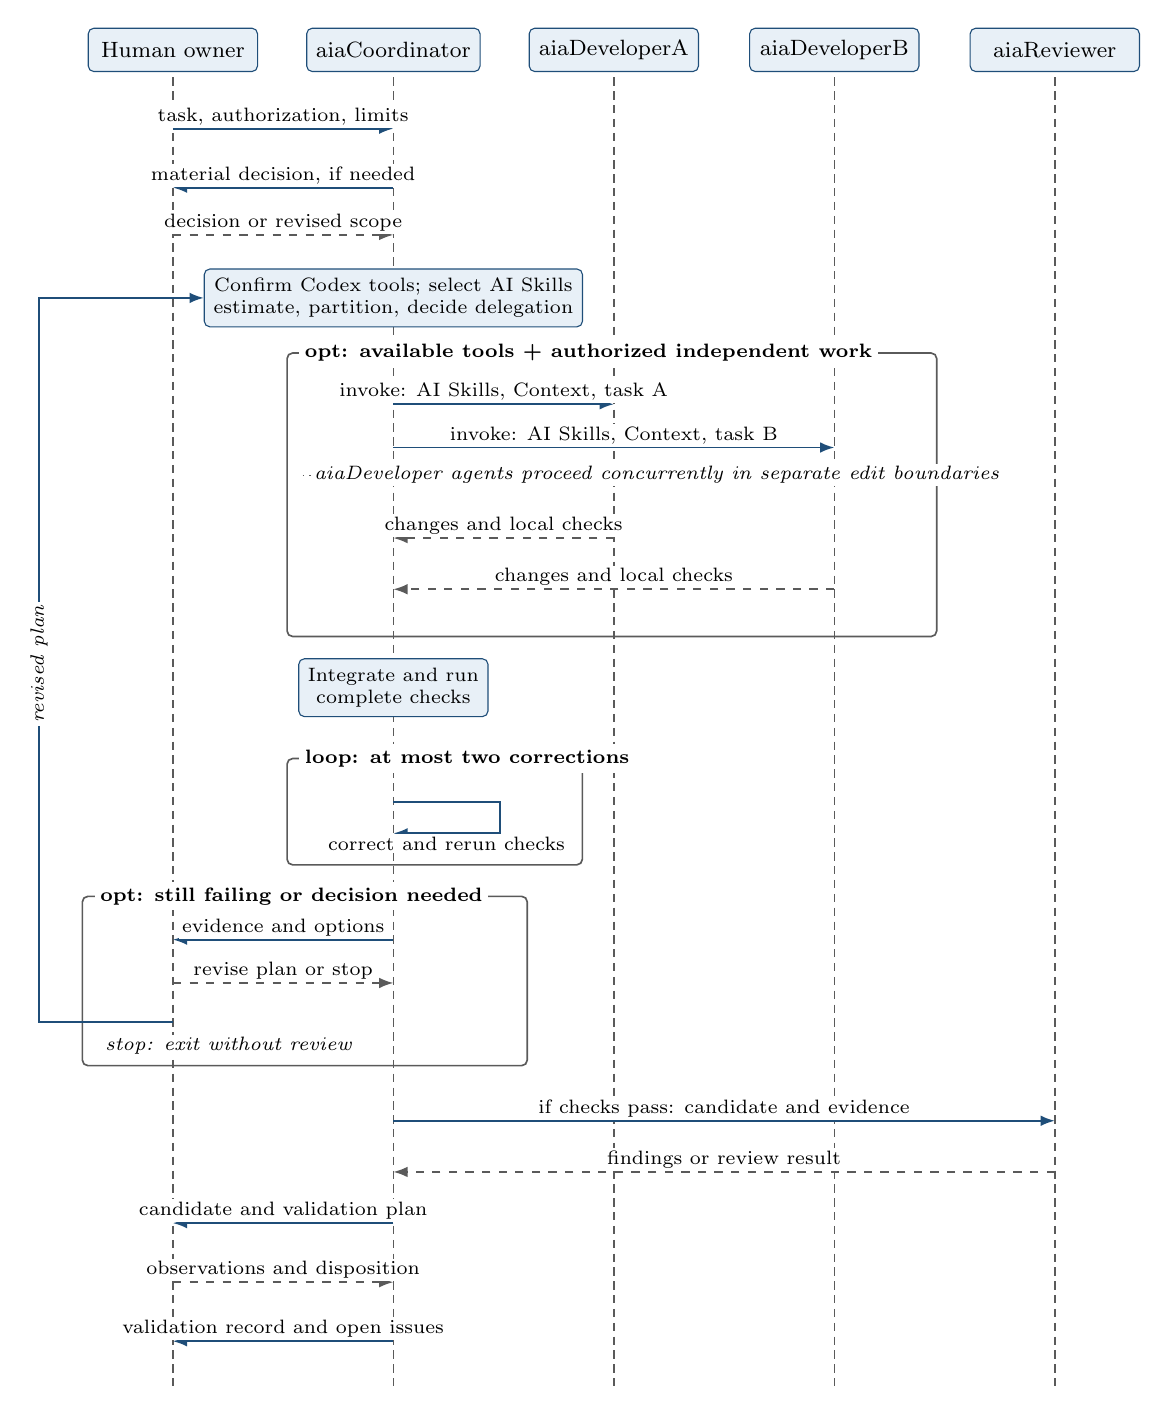
\begin{tikzpicture}[
  x=1cm,y=1cm,
  participant/.style={draw=s8sBlue,fill=s8sLightBlue,rounded corners=2pt,
    minimum width=2.15cm,minimum height=0.55cm,align=center,font=\footnotesize},
  lifeline/.style={draw=s8sGray,densely dashed,line width=0.55pt},
  msg/.style={-{Latex[length=1.8mm]},draw=s8sBlue,line width=0.65pt},
  response/.style={-{Latex[length=1.8mm]},draw=s8sGray,dashed,line width=0.65pt},
  note/.style={font=\scriptsize,fill=white,inner sep=1pt},
  frame/.style={draw=s8sGray,rounded corners=2pt,line width=0.6pt}
]
  \node[participant] at (0,0) {Human owner};
  \node[participant] at (2.8,0) {aiaCoordinator};
  \node[participant] at (5.6,0) {aiaDeveloperA};
  \node[participant] at (8.4,0) {aiaDeveloperB};
  \node[participant] at (11.2,0) {aiaReviewer};
  \foreach \x in {0,2.8,5.6,8.4,11.2}
    \draw[lifeline] (\x,-0.35) -- (\x,-17.0);

  \draw[msg] (0,-1.0) -- node[note,above] {task, authorization, limits} (2.8,-1.0);
  \draw[msg] (2.8,-1.75) -- node[note,above] {material decision, if needed} (0,-1.75);
  \draw[response] (0,-2.35) -- node[note,above] {decision or revised scope} (2.8,-2.35);

  \node[draw=s8sBlue,fill=s8sLightBlue,rounded corners=2pt,
    font=\scriptsize,align=center,minimum width=3.4cm]
    (delegationDecision) at (2.8,-3.15) {Confirm Codex tools; select AI Skills\\estimate, partition, decide delegation};

  \draw[frame] (1.45,-3.85) rectangle (9.7,-7.45);
  \node[anchor=west,font=\scriptsize\bfseries,fill=white,inner sep=2pt]
    at (1.6,-3.85) {opt: available tools + authorized independent work};
  \draw[msg] (2.8,-4.5) -- node[note,above] {invoke: AI Skills, Context, task A} (5.6,-4.5);
  \draw[msg] (2.8,-5.05) -- node[note,above] {invoke: AI Skills, Context, task B} (8.4,-5.05);
  \draw[s8sGray,dotted] (1.65,-5.4) -- (9.5,-5.4);
  \node[anchor=west,font=\scriptsize\itshape,fill=white,inner sep=1pt]
    at (1.75,-5.4) {aiaDeveloper agents proceed concurrently in separate edit boundaries};
  \draw[response] (5.6,-6.2) -- node[note,above] {changes and local checks} (2.8,-6.2);
  \draw[response] (8.4,-6.85) -- node[note,above] {changes and local checks} (2.8,-6.85);

  \node[draw=s8sBlue,fill=s8sLightBlue,rounded corners=2pt,
    font=\scriptsize,align=center,minimum width=2.4cm]
    at (2.8,-8.1) {Integrate and run\\complete checks};
  \draw[frame] (1.45,-9.0) rectangle (5.2,-10.35);
  \node[anchor=west,font=\scriptsize\bfseries,fill=white,inner sep=2pt]
    at (1.6,-9.0) {loop: at most two corrections};
  \draw[msg] (2.8,-9.55) -- ++(1.35,0) -- ++(0,-0.4) --
    node[note,below] {correct and rerun checks} (2.8,-9.95);

  \draw[frame] (-1.15,-10.75) rectangle (4.5,-12.9);
  \node[anchor=west,font=\scriptsize\bfseries,fill=white,inner sep=2pt]
    at (-1.0,-10.75) {opt: still failing or decision needed};
  \draw[msg] (2.8,-11.3) -- node[note,above] {evidence and options} (0,-11.3);
  \draw[response] (0,-11.85) -- node[note,above] {revise plan or stop} (2.8,-11.85);
  \draw[msg] (0,-12.35) -- (-1.7,-12.35) -- (-1.7,-3.15) -- (delegationDecision.west);
  \node[font=\scriptsize\itshape,fill=white,inner sep=1pt,rotate=90]
    at (-1.7,-7.8) {revised plan};
  \node[anchor=west,font=\scriptsize\itshape,fill=white,inner sep=1pt]
    at (-0.9,-12.65) {stop: exit without review};

  \draw[msg] (2.8,-13.6) -- node[note,above] {if checks pass: candidate and evidence} (11.2,-13.6);
  \draw[response] (11.2,-14.25) -- node[note,above] {findings or review result} (2.8,-14.25);
  \draw[msg] (2.8,-14.9) -- node[note,above] {candidate and validation plan} (0,-14.9);
  \draw[response] (0,-15.65) -- node[note,above] {observations and disposition} (2.8,-15.65);
  \draw[msg] (2.8,-16.4) -- node[note,above] {validation record and open issues} (0,-16.4);
\end{tikzpicture}
}
  \caption[AI-assisted development and validation handoffs.]{AI-assisted development and validation handoffs. Codex supplies subagent tools; the human authorizes delegation; the aiaCoordinator decides and invokes. Parallel aiaDeveloper agents are used only for independent tasks; otherwise the aiaCoordinator develops tasks sequentially.}
  \label{Figure:AIImplementationSequence}
\end{figure}

\begin{figure}[htbp]
  \centering
  \resizebox{\linewidth}{!}{% Shared by the architecture manual and Week 03 slides.
\providecommand{\AIActivityRef}[2]{\hyperref[#1]{#2}}
\providecommand{\AIActivityCColor}{s8sBlue}
\providecommand{\AIActivityDColor}{s8sGreen}
\providecommand{\AIActivityFlowColor}{s8sGray}
\begin{tikzpicture}[
  action/.style={rounded corners=2pt,text width=4.15cm,minimum height=1.45cm,
    inner sep=5pt,align=center,font=\fontsize{10}{12}\selectfont},
  ctask/.style={action,draw=\AIActivityCColor,fill=\AIActivityCColor!6},
  execution/.style={action,draw=\AIActivityDColor,fill=\AIActivityDColor!6},
  flow/.style={-{Stealth[length=2mm]},draw=\AIActivityFlowColor,line width=.8pt}
]
\node[ctask] (select) at (0,0) {\textbf{Appendix C: skills}\\
  \AIActivityRef{Table:AISkills}{Select AI Skills; read Context}\\
  \AIActivityRef{Section:AIArchitectureWorkflow}{Read Steps and Acceptance}};
\node[execution] (plan) at (5.05,0) {\textbf{Appendix D: plan}\\
  \AIActivityRef{Section:AIImplementationPlan}{Plan the selected tasks}\\
  \AIActivityRef{Section:AIAgentDelegation}{Choose one or multiple agents}};
\node[execution] (develop) at (10.1,0) {\textbf{Appendix D: develop}\\
  \AIActivityRef{Section:AIImplementationVerification}{Develop assigned tasks}\\
  Use the selected skill definitions};
\node[execution] (check) at (10.1,-3.0) {\textbf{Appendix D: check}\\
  \AIActivityRef{Section:AIImplementationVerification}{Integrate, verify, and review}\\
  \AIActivityRef{Section:AIImplementationValidation}{Validate when required}};
\node[ctask] (accept) at (5.05,-3.0) {\textbf{Appendix C: Acceptance}\\
  \AIActivityRef{Section:AIArchitectureWorkflow}{Check task Acceptance}\\
  \AIActivityRef{Table:AICompletionChecklist}{Apply completion checklist}};
\node[ctask] (report) at (0,-3.0) {\textbf{Appendix C: report}\\
  \AIActivityRef{Table:AICompletionChecklist}{Report results and evidence}\\
  List open decisions};
\node[circle,fill=\AIActivityFlowColor,inner sep=2.5pt] (start) at (-3,0) {};
\node[circle,draw=\AIActivityFlowColor,inner sep=3.5pt] (end) at (0,-4.5) {};
\node[circle,fill=\AIActivityFlowColor,inner sep=2pt] at (end.center) {};
\draw[flow] (start) -- (select);
\draw[flow] (select) -- (plan);
\draw[flow] (plan) -- (develop);
\draw[flow] (develop) -- (check);
\draw[flow] (check) -- (accept);
\draw[flow] (accept) -- (report);
\draw[flow] (report) -- (end);
\end{tikzpicture}
}
  \caption{Activity connecting Appendix C skill definitions and Acceptance to Appendix D execution. The agent-count decision belongs to Appendix D for every selected task.}
  \label{Figure:AITaskExecutionActivity}
\end{figure}

\chapter{AI Prompt Log}
\ChapterLabel{AIPromptLog}
\section{Chapter Responsibility}
\label{Section:AIPromptLogResponsibility}
Preserve supplied facts, AI drafting scope, and human-review boundaries.

\noindent\textbf{Expected result:} A reviewable project record with explicit evidence and gaps.


\section{AIS-02 Initialization: November 9, 2026}
The user asked Codex to instantiate template 2.33 in a separate directory,
review the facts and gaps before dependent edits, keep separate TikZ sources
and trace links, and return the complete build for review. The user confirmed
the project name, namespace, mission, scope, system boundary, stakeholders,
owners, and Embedded Systems applicability. The user specified the
publication destination and reserved acceptance and publication authorization
for a later step.

The confirmed facts and the prior project draft informed the candidate
chapters. Candidate requirements, priorities, and test designs remain draft.
Technical and evidence decisions are tracked in
\hyperref[Table:OwnedQuestions]{the owned questions}.

\section{Context Draft and Drawing (November 14, 2026)}
The user requested a context description and matching drawing that identify
external devices, the host application, the consumer, and what crosses each
boundary. The \hyperref[Section:MeasurementMission]{context draft} distinguishes
the control app boundary from the system boundary and links the missing
engineering results to the \hyperref[Table:OwnedQuestions]{owned questions}.

\section{Conversation Logging (November 19, 2026)}
After recovering three archived conversations and exporting timestamped
Markdown transcripts, the user requested an automatic project rule for
future conversations. \hyperref[Rule:AIChatLogging]{The conversation
transcript rule} defines the destination, verbatim content, timestamp format,
refresh points, and active-response limitation. The local exporter refreshes
available project conversations without committing or publishing them.

\section{Integrated Specification Publication (November 23, 2026)}
The user authorized restructuring the publication into a System Requirements
and Architecture Specification, retaining complete requirements and detailed
test, verification, validation, traceability, and evidence registers.
The publication scope is defined in
\path|s8sDocumentGuide.tex|. Existing artifact IDs and obligations are
preserved; unresolved decisions and Pending evidence remain explicit.

\section{Project Co-authorship (November 23, 2026)}
The user requested Chadwick Adebiyi as co-author of all project documents.
\hyperref[Section:ProjectAuthorship]{Project Authorship} records the decision;
the shared \texttt{DocumentAuthors} metadata supplies publication and
transcript-header credits. Repository authoring guidance applies the same
credit to future project documents while retaining verbatim historical
message bodies and original external-source attribution.

\section{Recording and Playback Stories (November 23, 2026)}
\label{Section:RecordingPlaybackPrompt}
The user asked which stakeholder stories could support recording sensor data
and playback for debugging. After reviewing the proposed stories, the user
accepted stories 5, 6, 7, 8, and 11 and requested their addition to the User
Stories chapter. AI skill \hyperref[Skill:AIS-05]{\texttt{AIS-05}} added
\UserStoryRef{US-05}, \UserStoryRef{US-06}, \UserStoryRef{US-07},
\UserStoryRef{US-08}, and \UserStoryRef{US-09} with their acceptance intent.
One agent performed the edit and self-review. No stories for result comparison
or recording export were added. No derived requirement approval, product
verification, stakeholder validation result, or release authorization is inferred.
The conversation's working directory is outside the source repository;
automatic transcript discovery does not capture this chat without an explicit
source export under \hyperref[Rule:AIChatLogging]{the transcript rule}.

The user subsequently requested consecutive story numbering and suggestions
for use cases and diagrams. The replay-output story originally proposed as
US-11 is now \UserStoryRef{US-09}; linked references were updated.
Use-case and diagram suggestions remain proposals pending selection.

\section{Recording and Playback Engineering Package (November 23, 2026)}
\label{Section:DiagnosticPackagePrompt}
The user requested requirements derived from the proposed use cases, requirement verifications and use-case validations, then authorized proceeding. One aiaCoordinator/aiaDeveloper performed the connected edits and self-review using \hyperref[Skill:AIS-01]{\texttt{AIS-01}}, \hyperref[Skill:AIS-05]{\texttt{AIS-05}}, \hyperref[Skill:AIS-06]{\texttt{AIS-06}}, \hyperref[Skill:AIS-07]{\texttt{AIS-07}}, \hyperref[Skill:AIS-08]{\texttt{AIS-08}}, \hyperref[Skill:AIS-09]{\texttt{AIS-09}}, \hyperref[Skill:AIS-11]{\texttt{AIS-11}}, \hyperref[Skill:AIS-13]{\texttt{AIS-13}} and \hyperref[Skill:AIS-14]{\texttt{AIS-14}}. No delegated or independent review is claimed. The plan was a sequential 15--25 minute authoring/checking effort: scenarios and diagrams approximately 5--10 minutes, 3,000--5,000 tokens; requirements and reciprocal plans 5--10 minutes, 4,000--7,000 tokens; compilation and self-review 5 minutes, 2,000--4,000 tokens, with uncertainty from layout and compiler diagnostics. Shared registers made delegation overhead unjustified. Quantitative limits, recording/compatibility policies, replay time/state and routing remain owned questions; all new requirements are Proposed and all execution dispositions Pending. Human technical review and stakeholder execution remain future work.

\section{Playback Review Corrections (November 25, 2026)}
\label{Section:PlaybackReviewCorrectionsPrompt}
The user requested review of PR 6, then authorized merging the changes into origin/main and updating the Architecture Specification. The review identified missing initialization on playback start/restart and ambiguous speed scaling. One aiaCoordinator/aiaDeveloper applied \hyperref[Skill:AIS-06]{\texttt{AIS-06}}, \hyperref[Skill:AIS-07]{\texttt{AIS-07}}, \hyperref[Skill:AIS-08]{\texttt{AIS-08}}, \hyperref[Skill:AIS-09]{\texttt{AIS-09}}, \hyperref[Skill:AIS-13]{\texttt{AIS-13}} and \hyperref[Skill:AIS-14]{\texttt{AIS-14}} sequentially, with self-review. No independent review, product execution, stakeholder acceptance or requirement-baseline approval is claimed. Initialization mechanisms and engineering policies remain owned decisions. The local transcript is refreshed under \hyperref[Rule:AIChatLogging]{the transcript rule}.

\section{Ordered Main Integration (November 25, 2026)}
The user clarified the workflow test: merge the Architecture Specification work first, then the updated user stories. The first merge reached origin/main as \texttt{e593772}. The user-story integration preserves the reader-publication structure, repository-only guidance, co-author metadata and generated \path|s8sArchitecture.pdf|. Conflicting history, prompt, evidence and scope text were reconciled without dropping either change. The superseded \path|s8sManual.pdf| remains removed. GitHub connector and CLI API merge attempts returned service errors before either merge; ordinary Git merges and pushes preserve the requested sequence.

\chapter{Test Evidence}
\ChapterLabel{TestEvidence}
\label{Section:TestEvidenceResponsibility}
This chapter distinguishes observed document-build evidence from absent product evidence.



\section{Product Evidence State}
No application has been implemented, no product test has been executed, and no verification or stakeholder validation result has been observed in this documentation stage. All \hyperref[Table:VerificationRegister]{verification records} and \hyperref[Table:ValidationRegister]{validation records} remain Pending. Planned tests are in \hyperref[Table:ProjectTests]{the test register}.

\section{Document Evidence}
Document-build and PDF-inspection evidence is recorded separately in the repository review source \href{s8sInstantiationReview.tex}{\texttt{s8sInstantiationReview.tex}}. This evidence concerns the authored book only. Future product records must identify test ID, requirement, implementation revision, fixture/hardware revision, platform/toolchain, procedure/command, input, expected and observed results, timestamp, operator, retained evidence path, and human disposition.

\chapter{Instantiation Review}
\ChapterLabel{InstantiationReview}
\section{Chapter Responsibility}
\label{Section:InstantiationReviewResponsibility}
Report AIS-02 evidence, checks, limitations, and required human dispositions.

\noindent\textbf{Expected result:} A reviewable project record with explicit evidence and gaps.


\section{Scope and Method}
\hyperref[Skill:AIS-02]{AIS-02} governs initialization. The
\hyperref[Table:ProjectDomainProfiles]{profile decision} guides embedded
tailoring, and \hyperref[Skill:AIS-13]{AIS-13} and
\hyperref[Skill:AIS-14]{AIS-14} guide consistency and build checks.
Codex drafted and self-reviewed the candidate sequentially because chapter
inputs and trace registers share dependencies. The prior draft supplies
stable IDs and trace mappings.

\section{Review Checks}
Run the complete build and source check from the project directory.
\begin{verbatim}
make -f s8sMakefileMacLinux pdf
python3 s8sCheckSources.py
\end{verbatim}
Check active inputs, naming, unique IDs, citations, and reciprocal mappings.
Review the final LaTeX log, render all pages, inspect figures and tables,
and check internal links. Compare the reusable template's file inventory
and hashes before and after authoring.

\section{Required Human Dispositions}
Michael Stoddard coordinates review and the
\hyperref[Table:OwnedQuestions]{owned questions}. Dr. Darian Muresan retains
technical acceptance authority. See the publication gate in \ChapterRef{Release}.

\chapter{Document History}
\ChapterLabel{DocumentHistory}
\section{Chapter Responsibility}
\label{Section:DocumentHistoryResponsibility}
Record the project draft evolution without inventing approval.

\noindent\textbf{Expected result:} A reviewable project record with explicit evidence and gaps.


\section{Project Draft History}
The prior SPE-800 project draft at Git commit \texttt{49c9020} provided the
starting point for project facts, open questions, and stable trace links.

Template lineage is archived in \path|s8sTemplateHistory.tex|.

\paragraph{November 9, 2026}
The user confirmed SPE-800-Sensor, namespace \texttt{s8s}, the documentation
scope and system boundary, stakeholders, owners, and the Embedded Systems
profile. AIS-02 established this standalone review candidate in
\path|Architecture/|. See \ChapterRef{AIPromptLog},
\ChapterRef{DevelopmentPlan}, and \ChapterRef{InstantiationReview}.

\paragraph{November 19, 2026}
The user requested routine verbatim conversation exports to
\path|docs/chats/| under Architecture, with timestamps on prompts and responses.
Added \hyperref[Rule:AIChatLogging]{the conversation transcript rule}, a local
exporter, and a thin Architecture discovery pointer. The rule states the
capture boundary for an active final response; no background service or
publication authorization is implied. See \ChapterRef{AIPromptLog}.


\setglossarystyle{altlist}
\glsaddall
\printglossaries

\bibliographystyle{IEEEtran}
\bibliography{s8sReferences}
\cleardoublepage
\phantomsection
\ChapterLabel{Index}
\addcontentsline{toc}{chapter}{Index}
\markboth{Index}{Index}
\printindex

\end{document}
